%----------------------------------------------------------------------------------------
%       CHAPTER 20
%----------------------------------------------------------------------------------------

\cleardoublepage

\chapterimage{ch-howto.png} % Chapter heading image

\chapter{HOW-TO (experiment)}\label{ch:how-to-experiment}

\hfill \break
\vspace{24mm}

\Large
What follows are potted HOW-TO instructions for doing things, split into more technical installing and running the model (previous Chapter) vs. configuring experiments (this Chapter).
\vspace{2mm}

There is some overlap with the FAQ Chapter, so please read all three!
\normalsize

%------------------------------------------------
\newpage
%------------------------------------------------

\section{HOW-TO ... diagnose how the system works}

This HOW-TO will:
\vspace{1mm}
\begin{enumerate}[noitemsep]
\item Implement a (single-tracer) water mass age tracer.
\item Implement a (dual-tracer) water mass age tracer. (Old scheme.)
\item Implement 'preformed' and other diagnostic biogeochemical cycling tracers.
\end{enumerate}

\noindent\rule{4cm}{0.5pt}
%------------------------------------------------

%------------------------------------------------
%
\newpage
\subsection*{Add a water mass age tracer}
\vspace{2mm}

To diagnose water mass age, a single diagnostic tracer is required -- \texttt{ocn\_colr} (tracer number \(48\)). Once selected (in the \textit{base-config}), you only then need set\footnote{(\texttt{bg\_ctrl\_force\_ocn\_age1} to distinguish it from the earlier scheme (\texttt{bg\_ctrl\_force\_ocn\_age}) that required 2 tracers.} (\textit{user-config}):
\vspace{-1mm}\small\begin{verbatim}
bg_ctrl_force_ocn_age1=.true.
\end{verbatim}\normalsize\vspace{-1mm}

The time-series output appears as file \textsf{\footnotesize biogem\_series\_misc\_col\_age.res}. 3D netCDF output is provided via the variable \texttt{misc\_col\_Dage} ('color tracer; ventilation age') with units of \(yr\).

The way it works is that initially the ocean everywhere has zero age\footnote{Hence, the total spin-up time needs to exceed the maximum age, for an ocean circulation at steady-state, or a run duration a factor several times this for a \textit{spin-up} from cold.}. Then each time-step, the water in every interior (excepting those at the surface) ocean grid cell is aged by the time-step duration. The ocean surface is continually restored to zero (age). A \textit{re-start} age distribution can be directly re-started from.

The advantage of this simplified age tracer (other than its simplicity!!!) is that it frees up the numerical 'blue' tracer for other purposes.

\noindent\rule{4cm}{0.5pt}
%------------------------------------------------

%------------------------------------------------
%
\newpage
\subsection*{Add a dual-tracer water mass age  (original, more complicated schemes)}
\vspace{2mm}

[Note that this is pretty much entirely superseded by the previously-described, single-tracer alternative.]

\vspace{1mm}
\noindent Water masses (and hence something of ocean circulation) can be tagged with a color (dye) tracer. However, on its own, this can tell you nothing about water mass age. A second color tracer can be added, however, and configured in such a way that by analysing the ratio of the two tracers, water mass age (time since a parcel of water last saw the surface ocean on average).

First off, you are going to need a \textit{base-config} that defines both color tracers. An example of this (but with no biology or carbon cycle and a modern configuration) is:
\vspace{-1mm}\small\begin{verbatim}
cgenie.eb_go_gs_ac_bg.worjh2.rb
\end{verbatim}\normalsize\vspace{-1mm}
Obviously, this can be adapted or the 2 lines selecting the 'red' and 'blue' color tracers, copied over into a different \textit{base-config} (but remembering that the total number of ocean tracers selected then increases by 2).

\vspace{1mm}
The way this is going to work is:

\begin{enumerate}
\setlength{\itemindent}{.2in}

\vspace{1mm}
\item A restoring of red dye is applied evenly to the entire ocean surface. By itself, this will simply result in the ocean progressively filling up with dye until equal to the surface concentration and with no time information.

\vspace{1mm}
\item So a blue dye is also injected. The concentration of this is also restored at the surface. However, the surface concentration of the blue dye is scaled such that it reflects age in the model experiment. This counts 'down', such that at the start of the experiment the dye is at its highest concentration and hence representing the greatest amount of time (age). As the run progressive and time runs towards zero, so does the dye flux. i.e. for for an experiment running for 10,000 years, the concentration of blue at the surface linearly declines from 10,000 to 0.
\\Or alternatively:

\vspace{1mm}
\item So far, even with the blue dye reflecting 'time', remote parts of the ocean will not have received much dye, so even though the water should be 'old' and the surface concentration high, the concentration and hence 'age' in the deep ocean will still be low. So the red dye is used to normalize for the dispersion and dilution of the blue dye.

\end{enumerate}
\vspace{2mm}

Water mass age tracing can be configured quite simply, and with the tracer concentration manipulations carried out automatically, as follows. As \textit{base-config} file with both red and blue color tracers defined is still required, but  rather than have to define and use a set of \textit{forcings} (and associated forcing configuration), a single parameter is added in the \textit{user-config} file:
\vspace{-1mm}\small\begin{verbatim}
bg_ctrl_force_ocn_age=.true.
\end{verbatim}\normalsize\vspace{-1mm}
This will automatically create the age tracer and additional explicitly output (in netCDF) both the total age of a water parcel, as well as the age relative to the surface (ventilation age).

In this methodology, in the netCDF output, the concentration ratio of blue/red, should be 'age' -- the mean time that a parcel of water was last at the surface.

In comparison, in the original (and still valid way of implementing water mass age tracing), 2 surface ocean \textit{forcings} need be specified in order to create the combined age tracer. An example forcing is provided: \textit{forcing}: \texttt{pyyyyz.Rcolr\_Rcolb}, which is then configured, for a 10,000 year run in this example, by adding the following 2 parameter settings in the \textit{user-config}:
\vspace{-1mm}\small\begin{verbatim}
bg_par_ocn_force_scale_val_49=10000.0
bg_par_ocn_force_scale_time_49=10000.0
\end{verbatim}\normalsize\vspace{-1mm}

\noindent (If the experiment duration is longer than 10,000 years, the parameter values need be adjusted accordingly.)

\vspace{1mm}
Example \textit{user-config} files for both approaches are provided:
\vspace{-1mm}\small\begin{verbatim}
EXAMPLE.worjh2.NONE_age.SPIN
EXAMPLE.worjh2.NONE_colage.SPIN
\end{verbatim}\normalsize\vspace{-1mm}

\noindent Note that the automatic approach (\texttt{EXAMPLE.worjh2.NONE\_colage.SPIN}) will handle experiments started from a \textit{re-start} (but not for the manual approach). The only advantage to the manual approach (\texttt{EXAMPLE.worjh2.NONE\_age.SPIN}), which is provided for backwards code/experiment compatibility, is that it is possible to specify a surface age for a specific region, e.g. North Atlantic, meaning that the ventilation age is the time since a parcel of water last saw the North Atlantic rather than anywhere at the surface (as in the automatic approach).

\noindent\rule{4cm}{0.5pt}
%------------------------------------------------

%------------------------------------------------
%
\newpage
\subsection*{Include 'preformed' tracers}
\vspace{1mm}

Preformed tracers are selected via 2 \textit{user-config} modifications:

\begin{enumerate}
\vspace{1mm}
\item By setting the parameter:
\vspace{-1mm}\small\begin{verbatim}
bg_ctrl_bio_preformed=.true.
\end{verbatim}\normalsize\vspace{-1mm}
\vspace{1mm}
\item By including sufficient/appropriate 'color' (numerical) tracers in the \textit{base-config}.
\end{enumerate}
\vspace{2mm}

\noindent A total of 10 generic 'color' tracers are defined and can be selected (in the \textit{base-config}), from \texttt{io\_col0} (tracer number \#57) through \texttt{io\_col9} (tracer number \#66), and with the preformed tracer parameter set \texttt{true}, represent:

\begin{table}[ht]
%\caption{Preformed tracers} % title of Table
%\centering % used for centering table
\begin{tabular}{l l l} % left-hand alligned columns (3 columns)
\hline\hline %inserts double horizontal lines
Ocean tracer number & Mnemonic & Represents the preformed version of the tracer \\ [0.5ex] % inserts table
%heading
\hline % inserts single horizontal line
57 & \texttt{io\_col0} & \(DIC\) \\
58 & \texttt{io\_col1} & \(ALK\) \\
59 & \texttt{io\_col2} & \(O_{2}\) \\
60 & \texttt{io\_col3} & \(PO_{4}\) \\
61 & \texttt{io\_col4} & \(NO_{3}\) \\
62 & \texttt{io\_col5} & \(Fe\) (i.e. \(Fe^{3+}\)) \uline{or} \(TDFe\) \\
63 & \texttt{io\_col6} & \(SiO_{2}\) \\
64 & \texttt{io\_col7} & \(\delta^{13}C\) of \(DIC\) \\
65 & \texttt{io\_col8} & \(\Delta^{14}C\) (of \(DIC\)) \uline{or} \(\delta^{13}C\) of \(C_{soft}\) \\
66 & \texttt{io\_col9} & \(C_{soft}\) \\
[1pt] % [1ex] adds vertical space
\hline %inserts single line
\end{tabular}
\label{tab:nonlin} % is used to refer this table in the text
\end{table}

\noindent (Obviously, you need to have the respective ocean tracer selected.)

One can have a generic \textit{base-config}, with all 10 possible color tracers selected, and then only for the selected corresponding tracers will a preformed tracer be simulated and output generated. Or one can just select the specific color tracer corresponding to a selected biogeochem. tracer.

\noindent For the \(C_{soft}\) tracer, in addition to the option:
\vspace{-1mm}\small\begin{verbatim}
bg_ctrl_bio_preformed=.true.
\end{verbatim}\normalsize\vspace{-1mm}
you also need to ensure that the redox diagnostics are saved\footnote{Unless you select a data save option that already includes this. But safest is to explicitly set this \texttt{true}.}:
\vspace{-1mm}\small\begin{verbatim}
ctrl_bio_remin_redox_save=.true.
\end{verbatim}\normalsize\vspace{-1mm}

You can also specify whether the \(C_{soft}\) tracer contains just the carbon remineralizated from \(POC\), or from both \(POC\) and \(DOC\). By default,  \(DOC\) is included in the \(C_{soft}\) tracer field. To exclude \(DOC\) from the regenerated \(DIC\) field, set:
\vspace{-1mm}\small\begin{verbatim}
ctrl_bio_preformed_CsoftPOConly=.true.
\end{verbatim}\normalsize\vspace{-1mm}
(by default the parameter is \texttt{false} and \(DOC\) is also included in accounting for remineralization).

Additionally, if \texttt{io\_col8}) is selected and radiocarbon (e.g. \texttt{io\_DIC\_14C}) \uline{is not}, then the \(\delta^{13}C\) of \(C_{soft}\) is accounted for.

\vspace{1mm}
\noindent\rule{4cm}{0.5pt}
\vspace{2mm}

\noindent Preformed tracer output is saved in both time-series and time-slice form.

\begin{itemize}[noitemsep]
\vspace{1mm}
\item In addition to the standard tracer output -- \textsf{\footnotesize biogem\_series\_ocn\_colx.res} (where \textsf{\footnotesize x} is one of \(0\) through \(9\)) -- time-series output is also saved under the files: \textsf{\footnotesize biogem\_series\_diag\_pre\_yy.res}, where \textsf{\footnotesize yy} is the preformed tracer short name. 
\\For isotopes, the latter output provides values in units of per mill (\permille) as well as \(mol\). (The former, only as \(mol\) and concentrations.)
\vspace{1mm}
\item \textbf{netCDF} output also includes the basic tracer values (as both 2D and 3D) -- \textsf{\footnotesize ocn\_colx.res} (where \textsf{\footnotesize x} is one of \(0\) through \(9\)), and additionally, a series of (3D only) outputs: \textsf{\footnotesize diag\_pre\_yy}, where \textsf{\footnotesize yy} is the preformed tracer short name. For isotopes, \textsf{\footnotesize diag\_pre\_yy} variables are in units of per mill (\permille).\footnote{Note that the \(\delta^{13}C\) of \(C_{soft}\) is the isotopic value of the remineralized carbon, \uline{not} the contribution to \(\delta^{13}C\) of \(DIC\). See following section.}
\end{itemize}
\vspace{1mm}
i.e. for both time-series and time-slice output, the \textsf{\footnotesize diag\_pre} forms of output are the recommended ones.

\vspace{1mm}
\noindent Note that technically, \(C_{soft}\) is not a 'preformed' tracer but rather a 'remineralized' tracer. However, for easy of grouping the primary color tracer output together, ti takes the same prefix as the other tracers in the saved variable notation.

\vspace{1mm}
\noindent\rule{4cm}{0.5pt}
\vspace{2mm}

\noindent A variety of 'derived' output are also included (depending on tracer selection) in both \textit{time-series} and \textit{time-slice} formats. Most (if not all) of the \textit{time-series} variables are provided as a  sort of check of tracer integrity (and to save on further processing.)

\vspace{1mm}
\begin{itemize}[noitemsep]

\vspace{1mm}
\item [\textbf{time-series}]:
\begin{enumerate}[noitemsep]
\vspace{1mm}
\item \textsf{\footnotesize diag\_reg\_13Csoft} -- \(\delta^{13}C\) of \(C_{soft}\)
\vspace{1mm}
\item \textsf{\footnotesize diag\_reg\_13CsoftPLUSpre13C} -- \(\delta^{13}C\) of \(C_{soft}\) plus \(\delta^{13}C\) of preformed \(DIC\). 
\\In the absence of \(CaCO_{3}\), this should be equal to (mean ocean) \(DIC\) \(\delta^{13}C\).
\vspace{1mm}
\item \textsf{\footnotesize diag\_reg\_CsoftPLUSpreDIC} -- \(C_{soft}\) \uline{plus} preformed \(DIC\).
\\In the absence of \(CaCO_{3}\), this should be equal to (mean ocean) \(DIC\).
\vspace{1mm}
\item \textsf{\footnotesize diag\_reg\_O2PCsoftPLUSpreO2} -- \(C_{soft}\) converted to respired \(O_{2}\) via the \(C:O_{2}\) Redfield ratio, \uline{plus} preformed \(O_{2}\).
\\This should be equal to (mean ocean) \(O_{2}\).
\vspace{1mm}
\item \textsf{\footnotesize diag\_reg\_PCsoftPLUSprePO4} -- \(C_{soft}\) converted to regenerated \(PO_{4}\) via the \(C:PO_{4}\) Redfield ratio, \uline{plus} preformed \(PO_{4}\).
\\This should be equal to (mean ocean) \(PO_{4}\).
\end{enumerate}

\vspace{1mm}
\item [\textbf{time-slices}]:
\begin{enumerate}[noitemsep]
\vspace{1mm}
\item \textsf{\footnotesize diag\_reg\_O2sat} -- \(O_{2(sat)}\) -- \(O_{2}\) solubility calculated at every grid point using ambient (\(T,S\)).
\vspace{1mm}
\item \textsf{\footnotesize diag\_reg\_AOU} -- \(AOU\) -- estimated from  \(O_{2(sat)}\) minus  'real' \(O_{2}\) (\texttt{io\_O2}).
\vspace{1mm}
\item \textsf{\footnotesize diag\_reg\_AOU\_P} -- regenerated \(P\) -- estimated from \(AOU\) multiplied by the \(P:O_{2}\) Redfield ratio.
\vspace{1mm}
\item \textsf{\footnotesize diag\_reg\_AOU\_P\_C} -- regenerated \(C\) -- estimated from \(AOU\) multiplied by the \(P:O_{2}\) Redfield ratio and then the \(C:P\) ratio.
\vspace{1mm}
\item \textsf{\footnotesize diag\_reg\_AOU\_P\_C\_d13C} -- regenerated \(\delta^{13}C\) -- estimated from \(AOU\) multiplied by the \(P:O_{2}\) Redfield ratio and then the \(C:P\) ratio and then multiplied by \(\delta^{13}C\) of (overlying ocean) export \(POC\) ... to the moon!
\\The isotopic value is 'diluted' in the proportion of regenerated \(C\) over \(DIC\). i.e. it is an estimate (from \(AOU)\) of the \(DIC\) \(\delta^{13}C\) contribution from respired carbon.
\vspace{1mm}
\item \textsf{\footnotesize diag\_reg\_OU} -- 'real' oxygen utilization (\(OU\)) -- calculated as preformed \(O_{2}\) minus 'real' \(O_{2}\) (\texttt{io\_O2}).
\vspace{1mm}
\item \textsf{\footnotesize diag\_reg\_P} -- 'real' regenerated \(P\) -- calculated as actual \(PO_{4}\) (\texttt{io\_PO4}) minus preformed \(P\).
\vspace{1mm}
\item \textsf{\footnotesize diag\_reg\_P\_C} -- regenerated \(C\) -- estimated as regenerated \(P\) multiplied by the \(C:P\) Redfield ratio.
\vspace{1mm}
\item \textsf{\footnotesize diag\_reg\_P\_C\_d13C} -- regenerated \(\delta^{13}C\) -- estimated from regenerated \(P\) multiplied by the \(C:P\) Redfield ratio and then multiplied by \(\delta^{13}C\) of (overlying ocean) export \(POC\). 
\\The isotopic value is 'diluted' in the proportion of regenerated \(C\) over \(DIC\).
\vspace{1mm}
\item \textsf{\footnotesize diag\_reg\_C} -- regenerated \(C\) -- this is a simple copy of the \(C_{soft}\) tracer for completeness and is 'real' regenerated \(C\).
\vspace{1mm}
\item \textsf{\footnotesize diag\_reg\_C\_d13C} -- regenerated \(\delta^{13}C\) -- perhaps a little pointlessly ... estimated from ('real') regenerated \(C\) (aka \(C_{soft}\)) multiplied by \(\delta^{13}C\) of (overlying ocean) export \(POC\).
\\The isotopic value is 'diluted' in the proportion of regenerated \(C\) over \(DIC\).
\vspace{1mm}
\item \textsf{\footnotesize diag\_reg\_d13C} -- regenerated \(\delta^{13}C\) -- this is simply the \(C_{soft}\) \(\delta^{13}C\) tracer, \uline{but}, 'diluted' in the proportion of regenerated \(C\) over \(DIC\). i.e. it is an explicit (and 'real') measure of the \(\delta^{13}C\) contribution of respired carbon to \(DIC\).
\vspace{1mm}
\item \textsf{\footnotesize diag\_reg\_DIC} -- \(DIC\) (not really 'regenerated' \textit{per se}) -- calculated as the sum of preformed \(C\) plus regenerated \(C\).
\\This is provided as a simple 'check' on the tracers, and in the absence of \(CaCO_{3}\), should be equal to 'real' \(DIC\) (\texttt{io\_DIC}).
\vspace{1mm}
\item \textsf{\footnotesize diag\_reg\_DIC\_d13C} -- \(\delta^{13}C\) of \(DIC\) (not really 'regenerated' \textit{per se}) -- calculated as the weighted sum of preformed \(C\) plus regenerated \(C\) \(\delta^{13}C\).
\\This is provided as a simple 'check' on the tracers, and in the absence of \(CaCO_{3}\), should be equal to 'real' \(DIC\) \(\delta^{13}C\) (\texttt{io\_DIC\_13C}).
\end{enumerate}

\end{itemize}






%------------------------------------------------
%
\newpage
\subsection*{Diagnose a Transport Matrix}
\vspace{1mm}

The physical circulation in \textbf{muffin} can be diagnosed as a Transport Matrix: a representation of the steady-state average circulation as a sparse matrix (see \textit{Khatiwala et al.} [2005] Accelerated simulation of passive tracers in ocean circulation models. Ocean Modelling. 9 (1), pp. 51 - 69). There are a number of advantages of using a transport matrix such as finding preformed tracer distributions and using it as a surrogate circulation for a steady-state biogeochemical model (see \textit{Khatiwala} [2007] -- A computational framework for simulation of biogeochemical tracers in the ocean. Global Biogeochemical Cycles. 21 (3), GB3001).

At its most simplest, the method sets a passive tracer (i.e., affected by ocean circulation only) to 1 $\mu$mol kg$^{-1}$ in a single grid-box, leaving every other grid-box as 0 $\mu$mol kg$^{-1}$. The model is then integrated for a single timestep. The whole grid is then vectorised, i.e., grid-boxes are stacked on top of each other, and this forms one column of the matrix. This process is repeated for the next grid-box along forming the second column. The columns of the matrix represent the distribution of the tracer from each grid-box individually after one timestep. To diagnose a matrix within GENIE, a few extra steps are taken: 6 tracers are used in a gridded pattern to diagnose one depth level simultaneously; each depth level is diagnosed and averaged in a year in turn as the number of grid-boxes affected by convection is not predictable.

%------------------------------------------------
%
\subsubsection{Diagnosing within a GENIE run}
\vspace{1mm}

A full matrix can be diagnosed within a single run. To do so, first add the following six "colour" tracers selected to the \textit{base-config} file:
\vspace{-1mm}\small\begin{verbatim}
gm_ocn_select_57=.true.
gm_ocn_select_58=.true.
gm_ocn_select_59=.true.
gm_ocn_select_60=.true.
gm_ocn_select_61=.true.
gm_ocn_select_62=.true.
\end{verbatim}\normalsize\vspace{-1mm}
\noindent (and remembering to increase the total number of selected ocean tracers). 

Then in the \textit{user-config} file, set the following parameters values in order to diagnose a transport matrix:

\begin{enumerate}
\vspace{1mm}
\item By ensuring preformed tracers are not implemented:
\vspace{-1mm}\small\begin{verbatim}
bg_ctrl_bio_preformed=.false.
\end{verbatim}\normalsize\vspace{-1mm}
\vspace{1mm}
\item Select the transport matrix flag:
\vspace{-1mm}\small\begin{verbatim}
bg_ctrl_data_diagnose_TM=.true.
\end{verbatim}\normalsize\vspace{-1mm}
\vspace{1mm}
\item Select the year to start diagnosing the matrix. The matrix requires the same number of years to diagnose as there are depth levels in the configuration, e.g., 16 years with a 16-level configuration.
\vspace{-1mm}\small\begin{verbatim}
bg_par_data_TM_start=9980
\end{verbatim}\normalsize\vspace{-1mm}
\vspace{1mm}
\item Select the averaging interval. Setting to 1 will give one annual average matrix, 4 will give four seasonally averaged matrices and 12 will give monthly averaged matrices.
\vspace{-1mm}\small\begin{verbatim}
bg_par_data_TM_avg_n=1
\end{verbatim}\normalsize\vspace{-1mm}
\end{enumerate}
\vspace{2mm}

\noindent There are also a few other things to consider. The model will try and warn you...

\begin{itemize}
\vspace{1mm}
\item The "colour" tracers are used for other purposes such as preformed tracers. Diagnosing preformed tracers at the same time probably isn't a good idea.
\vspace{-1mm}\small\begin{verbatim}
bg_ctrl_bio_preformed=.false.
\end{verbatim}\normalsize\vspace{-1mm}
\item If you want to diagnose seasonal or monthly matrices, ensure you have seasonal variability otherwise you get will get a number of identical matrices:
\vspace{-1mm}\small\begin{verbatim}
ea_dosc=.true.
go_dosc=.true.
gs_dosc=.true.
\end{verbatim}\normalsize\vspace{-1mm}
\item If you want to diagnose seasonal or monthly matrices, you may want to save other output at the same intervals by setting the following (this is not the same as the matrix averaging parameter! Set to 24 for seasonal or 8 for monthly):
\vspace{-1mm}\small\begin{verbatim}
bg_par_data_save_slice_n=24
\end{verbatim}\normalsize\vspace{-1mm}
\end{itemize}

\noindent Lastly, \textbf{biogem} needs to run with a 1:1 time-step ratio with \textbf{goldstein}. You can either edit the \texttt{runmuffin.sh} script yourself or better, use the \texttt{runmuffin.TM.sh} script which sets this ratio to 1 automatically.

The transport matrix data will be written to a netCDF file named \texttt{transport\_matrix\_COO.nc} in the biogem output (\texttt{COO} stands for the specific format of the sparse matrix). See the next sections on what to do with it...

%------------------------------------------------

\subsubsection{Loading the Transport Matrix in MATLAB}

To load the Transport Matrix into MATLAB, copy \texttt{transport\_matrix\_COO.nc} to a directory MATLAB can see. Use the  \texttt{load\_genie\_matrix.m}  script from \url{www.github.com/derpycode/muffindata/Transport_Matrix} to read the file and create the matrix in \textbf{MATLAB} and save the matrices to a file  whatever you specified. A matrix is conventionally called \texttt{A}. If there are multiple matrices, they are saved under one file as \texttt{A1}, \texttt{A2} etc... e.g.
\vspace{-1mm}\small\begin{verbatim}
load_genie_matrix ( 'transport_matrix_COO.nc' , 'output_filename')
\end{verbatim}\normalsize\vspace{-1mm}
\noindent The script also saves a file called \texttt{matrix\_vars.mat} containing metadata:

\vspace{2mm}
\begin{enumerate}
\item \texttt{v\_index} - a structure array with 4 vectors containing the indices for longitude (\texttt{i}), latitude (\texttt{j}) and depth (\texttt{k} with 16 as surface, \texttt{rk} with 1 as surface). These are required to convert between a 3-D grid to vector formats (see below).
\item \texttt{nb} - the number of wet grid-boxes
\item \texttt{Ib} and \texttt{Ii} - indices containing the location of the surface and interior ocean grid-boxes in the matrix
\end{enumerate}
\vspace{2mm}

You should perform a basic check on the transport matrices before using them to check there were no issues in diagnosing them. Each row of the matrix must sum to 1.0 to ensure mass conservation. In practice, due to the way the matrix is averaged over a single run, this is never exact but should be close within several decimal places. Running \texttt{sum(A,2)} will find the sum of each row. \texttt{sum(sum(A,2))} should also equal the total number of boxes \texttt{nb}. Hopefully, it should be obvious that the circulation should be as close to steady state as possible in your run!

%------------------------------------------------
%
\subsubsection{Useful MATLAB Functions}
\vspace{1mm}

Additional MATLAB functions to help process and use transport matrices can be found at \url{www.github.com/derpycode/muffindata/Transport_Matrix}.

\vspace{2mm}
\begin{enumerate}
\item \texttt{v2f.m} and \texttt{f2v.m} - convert between vector and 3-D grid. Takes the vector indices in \texttt{v\_index} as arguments.
\item \texttt{read\_genie\_netcdf.m} - reads one or multiple variables from a genie netCDF output file into your MATLAB workspace. It will read in a 3-D field or convert to a vector format.
\item \texttt{split\_transport\_matrix.m} - splits a transport matrix into a boundary (surface grid-boxes only) and interior matrices, needed when solving for steady state solutions. The function takes the \texttt{Ib} variable as an argument.
\end{enumerate}
\vspace{2mm}

%------------------------------------------------

\newpage

%------------------------------------------------

\section{HOW-TO ... screw with the climate system}
\vspace{2mm}

\noindent\rule{4cm}{0.5pt}

%------------------------------------------------
%
\newpage
\subsection*{Set/un-set seasonal insolation forcing}
\vspace{1mm}

Seasonal insolation forcing of the \textbf{EMBM}, \textbf{GOLDSTEIN} ocean, and sea-ice model, are set by the following parameters\footnote{These are typically set in the \textit{base-config} if needed (i.e. different from default).}:
\vspace{-1mm}\small\begin{verbatim}
ea_dosc=.true.
go_dosc=.true.
gs_dosc=.true.
\end{verbatim}\normalsize\vspace{-1mm}
and are \texttt{.true.} by default.
To set an annual average insolation forcing with no seasonality, simply set these to \texttt{.false.}

\noindent\rule{4cm}{0.5pt}

%------------------------------------------------
%
\newpage
\subsection*{Implement 'brine-rejection'}
\vspace{1mm}

\textbf{muffin} has the capability to include this effect (at least crudely) and similarly to \textit{Bouttes et al.} [2010]. For this, three namelist parameter values need to be set:

\vspace{-2mm}\begin{verbatim}
bg_ctrl_force_GOLDSTEInTS=.TRUE.
bg_par_misc_brinerejection_frac=0.1
bg_par_misc_brinerejection_jmax=9
\end{verbatim}\vspace{-2mm}
The first, simply allows the \textbf{BIOGEM} biogeochem. module to directly influence ocean circulation. The second is the fraction of salt, rejected during sea-ice formation (e.g., see \textit{Bouttes et al.} [2010]) that is transferred directly to the bottom-most (underlying) ocean cell in the model. The third sets a latitude limit (counted in cells) to the effect -- on a \(18\times18\) grid, a value of 9 will restrict brine rejection to the southern hemisphere (and hence Southern Ocean); a value of 18 will allow it to take  place in the North Atlantic as well. (Note that in e.g., \textit{Bouttes et al.} [2010], the effect of brine-rejection is considered only in the Southern Ocean.)

There is also option for treating all tracers the same way (including DIC ALK, PO4, etc.) and translocate biogeochem. tracers proportionally to salinity.

\noindent\rule{4cm}{0.5pt}

%------------------------------------------------
%
\newpage
\subsection*{Add/modify geothermal heating'}
\vspace{1mm}

(see: \textit{HOW-TO ... force the system})

\noindent\rule{4cm}{0.5pt}

%------------------------------------------------

\newpage

%------------------------------------------------

\section{HOW-TO ...  iron (and dust)}

This HOW-TO will:
\vspace{1mm}
\begin{enumerate}[noitemsep]
\item Provide an overview of the different marine iron cycle schemes in \textbf{muffin}.
\item Describe the different options  for tracers describing the main players in marine iron cycle.
\item Detail the various calibrated parameter sets.
\item Describe alternative ways of prescribing the solubility of iron in dust.
\item Introduce ... fake dust(!) (for paleo configurations).
\item Describe other sources of dissolved iron to the ocean.
\end{enumerate}

%------------------------------------------------
%
\noindent\rule{4cm}{0.5pt}
\subsubsection{Overview of  marine iron cycle schemes in muffin}
\vspace{1mm}

There are 3 different ways of describing the marine iron cycle in terms of which tracers in the ocean are defined (described immediately below). These are associated with one or more alternative tunings of the primary parameters controlling iron cycling -- the solubility of iron in dust and the rate of scavenging of dissolved iron onto particulate organic matter, plus, some parameter scaling the characteristic biological nutrient (\(PO^{2-}_{4}\)) uptake time-scale (described subsequently). In theory, the different tracer configurations are interchangeable and either could be used in conjunction with any given tuned parameter set. However, in practice and in publications, specific tuned parameter sets have been associated with a specific tracer combination choice (and e.g. not tested equally with both). The various available marine iron cycle configurations are summarized in Table \ref{tab:ironconfigs}.

\vspace{-4mm}
\begin{table}[h]
\textbf{\caption{muffin iron cycle configurations\label{tab:ironconfigs}}}
\begin{tabular}{|p{0.375cm}||p{1.875cm}|p{1.25cm}||p{1.0cm}|p{1.0cm}||p{1.0cm}|p{1.0cm}|p{1.75cm}||p{3.25cm}|}\hline
\# & \textbf{Tracers} & Scheme & \(DOM_{\tau}\) (\(yr\))  & \(bio_{\tau}\) (\(d\)) & \(Fe_{sol}\) (\%) & \(k_{scav}\) & Dust field & \textbf{References} \\\hline
\hline
1 & \(Fe\), \(L\), \(FeL\) & \texttt{OLD} & 1.0 & 63.3 & 0.291 & 1.34 & Mahowald & \textit{\small Tagliabue et al.} \small{[2016]} \newline \textit{\smallÖdalen et al.} \small{[2020]} \newline \textit{\small Rae et al.} \small{[2020]} \\\hline
2 & \(Fe\), \(L\), \(FeL\) & \texttt{OLD} & 1.0 & 63.3 & 0.291 & 1.34 & (various) & \textit{\small Lambert, et al.} \small{[2021]} \\\hline
3 & \(Fe\), \(L\), \(FeL\) & (\texttt{OLD}) & 1.0 & 63.3 & n/a & n/a & (none) & \textit{\small Meyer et al.} \small{[2016]}  \newline \textit{Hülse et al.} \small{[2019]} \\\hline
4 & \(TDFe\), \(TL\) & \texttt{hybrid} & 1.0 & 95.6 & 0.201 & 0.344 & Mahowald & \textit{\small Ward et al.} \small{[2018]} \\\hline
5 & \(TDFe\), \(TL\) & \texttt{hybrid} & 1.0 & n/a & 0.201 & 0.344 & Mahowald & \textit{\small Ward et al.} \small{[2018]} \\\hline
6 & \(TDFe\), \(TL\) & \texttt{hybrid} & 0.5 & 60.0 \newline 60.0 & 0.125 \newline 0.244 & 0.225 \newline 0.225 & Mahowald \newline Albani & \textit{\small De'Ath et al.} \small{[in prep]} \\\hline
7 & \(TDFe\), \(TL\) & \texttt{hybrid} & 0.5 & 60.0 \newline 60.0 & \textit{0.100} \newline \textit{0.195} & 0.100 \newline 0.100 & Mahowald \newline Albani & \textit{\small De'Ath et al.} \small{[in prep]} \\\hline
8 & \(TDFe\), \(TL\) & \texttt{hybrid} & 0.5 & 60.0 & 0.244 & 0.225 & Albani & \textit{\small Ödalen et al.} \small{[in prep]} \\\hline
9 & \(TDFe\), \(TL\) & \texttt{hybrid} & 0.5 & n/a & 0.244 & 0.225 & Albani & \textit{\small Jones et al.} \small{[in prep]} \\\hline
10 & \(Fe\), \(Fe2\), \(TL\) & \texttt{FeFe2TL} & 0.5 & 63.3 & n/a & 0.344 & (none) & \textit{\small van de Velde et al.} \small{[2021]} \\\hline
\end{tabular}
\end{table}

\noindent \small NOTES: \normalsize
\vspace{1mm}
\footnotesize
\begin{itemize}[noitemsep]
\setlength{\itemindent}{-.15in}
\item [\#3] -- The tracers are present, but the iron cycle is 'disabled' so that the biological scheme operates with no \(Fe\) limitation.
\item [\#5] -- There is no \(bio_{\tau}\) value because the \textbf{ECOGEM} module is used.
\item [\#7] -- Tests an assumption of a spatially uniform iron solubility (\(Fe_{sol}\) values in italics).
\item [\#9] -- There is no single \(bio_{\tau}\) value (the biological scheme is split into diatoms and non-diatoms).
\item [\#10] -- In this study/configuration, dissolved iron is supplied hydrothermally (as reduced, \(Fe^{II}\)) at the seafloor, and additionally, optionally as oxidized \(Fe^{III}\) to the ocean surface (\textit{in lieu} of the solubilized component in dust and/or via rivers from terrestrial weathering).
\end{itemize}
\normalsize

%------------------------------------------------
%
\noindent\rule{4cm}{0.5pt}
\subsubsection{Iron schemes and tracer configurations}
\vspace{2mm}

In the original iron cycle in \textbf{muffin},  3 separate tracers were defined:
\vspace{1mm}
\begin{itemize}[noitemsep]
\item [\(Fe\)] -- free dissolved iron
\item [\(L\)] -- free ligands
\item [\(FeL\)] -- iron bound to ligands
\end{itemize}
\vspace{2mm}
The associated tracer selection in the \textit{base-config} looks like:
\small\vspace{-2pt}\begin{verbatim}
gm_ocn_select_9=.true.      #   Fe -- 'dissolved iron (Fe)'
gm_ocn_select_23=.true.     #   FeL -- 'ligand-bound Fe'
gm_ocn_select_24=.true.     #   L -- 'free ligand (iron binding)' 
\end{verbatim}\vspace{-2pt}\normalsize

However, because the equilibrium between these tracers is re-solved every time-step (and used to determine the free \(Fe\) concentration for scavenging), there is redundancy, and in practice, only 2 tracers are needed. Subsequent iron cycle scheme hence use only 2 tracers:
\vspace{1mm}
\begin{itemize}[noitemsep]
\item [\(TDFe\)] -- total dissolved iron, including iron bound to ligands
\item [\(TL\)] -- total dissolved ligand concentration (both free and bound to iron)
\end{itemize}
\vspace{2mm}

The associated tracer selection in the \textit{base-config} then looks like:
\small\vspace{-2pt}\begin{verbatim}
gm_ocn_select_90=.true.     #   TDFe -- 'total dissolved Fe'
gm_ocn_select_42=.true.     #   TL -- 'total dissolved ligand'
\end{verbatim}\vspace{-2pt}\normalsize

At each time-step, the concentration of 'free' iron (and iron bound to ligands) is solved for and used to calculate iron removal though scavenging.

But ... to distinguish between reduced (\(Fe^{II}\)) and oxidized (\(Fe^{III}\)) iron as well as account for the role of ligands ... 3 tracers are needed again (a sort of combination of the above two permutations):
\vspace{1mm}
\begin{itemize}[noitemsep]
\item [\(Fe\)] -- total dissolved iron III, including iron bound to ligands
\item [\(Fe2\)] -- total dissolved iron II (does not bind to ligands)
\item [\(TL\)] --  total dissolved ligand concentration (both free and bound to iron III)
\end{itemize} 
\vspace{2mm}
or as tracers:
\small\vspace{-2pt}\begin{verbatim}
gm_ocn_select_9=.true.      #   Fe -- 'dissolved iron III (Fe)'
gm_ocn_select_83=.true.     #   Fe -- 'dissolved iron II (Fe)'
gm_ocn_select_42=.true.     #   TL -- 'total dissolved ligand' 
\end{verbatim}\vspace{-2pt}\normalsize

\vspace{1mm}
\noindent\rule{4cm}{0.5pt}
\vspace{2mm}

\noindent Associated with these different sets of tracer and iron cycle configurations, are several different schemes for how the iron cycle is parameterized:

\begin{itemize}[noitemsep]
\vspace{1mm}
\item [\texttt{OLD}] -- The very original scheme -- based on 3 tracers (free iron, free ligand, ligand-bound iron), solves the equilibrium between them and based on this, scavenges free \(Fe\) from the water column, by any or all of: particulate organic matter, \(CaCO_{3}\), opal, and/or detrital matter.
\\Note that surface layer scavenging is calculated within \texttt{sub\_calc\_bio\_uptake} rather than as part of particulate remineralization subroutine (\texttt{sub\_calc\_bio\_uptake}).
\\Iron speciation (\(Fe\), \(FeL\), and \(L\)) is updated within the main \textbf{BIOGEM} loop.
\\This scheme  was used e.g. in the 'FeMIP' paper of \textit{Tagliabue et al.} [2016].
\vspace{1mm}
\item [\texttt{ALT}] -- As per \texttt{OLD}, but with surface layer scavenging  calculated within the particulate remineralization subroutine (\texttt{sub\_calc\_bio\_uptake}).
\\Iron speciation (\(Fe\), \(FeL\), and \(L\)) is updated within  particulate remineralization subroutine (sub\_calc\_bio\_uptake).
\\This scheme has not yet been published with(!) although it should be very little different (if at all) from \texttt{OLD}. (Numerically, it is preferable to \texttt{OLD}.) 
\vspace{1mm}
\item [\texttt{hybrid}] -- As per \texttt{ALT}, but employing only 2 tracers -- total dissolved iron, and total dissolved ligand (and solving for the equilibrium between (free iron, free ligand, and ligand-bound iron).
\\This is the recommenced modern modern (oxic ocean) configuration option (e.g. as used by \textit{Ward et al.} [2018]). 
\\In theory ... it should be identical in behavior to \texttt{ALT} (but with one fewer tracer simulated in the ocean).
\vspace{1mm}
\item [\texttt{lookup\_4D}] -- Yet to be fully implemented/published ... this assumes 2 tracers in the ocean (total dissolved iron, total dissolved ligand) and calculates the equilibrium partitioning between dissolved iron and solid FeOOH (assumed to be goethite), based on ambient temperature and pH (in addition to total dissolved iron, total dissolved ligand) and employing a lookup table. Solid FeOOH is the phase that is scavenged.
\vspace{1mm}
\item [\texttt{FeFe2TL}] -- A 3-phase tracer scheme, but distinguishing the oxidized form \(Fe^{III}\) (tracer: \texttt{Fe}) from reduced \(Fe^{II}\) (tracer: \texttt{Fe2})\footnote{In the water column, \(Fe^{II}\) oxidizes to \(Fe^{III}\) under oxic conditions, while \(Fe^{III}\) is reduced under anoxic conditions.}. This scheme is primarily intended for predominantly ferruginous/euxinic deeper time esp. Precambrian) oceans, but is perfectly capable of being used in more geologically recent and predominantly oxic ocean times (as well as more 'mixed state' oceans, such as during OAEs or during the Paleozoic).
\\Only \(Fe^{III}\) (tracer: \texttt{Fe}) is taken into account in the calculation for  partitioning iron into free and ligand-bound iron, and only free (non ligand-bound) \(Fe^{III}\) is then subject to scavenging. Reduced \(Fe^{II}\) (tracer: \texttt{Fe2}) is assumed truly dissolved and does not bind with ligands, nor is subject to scavenging.
\\In principal, in the absence of \texttt{is\_POM\_FeOOH}, the marine iron cycle should function identically to the original 'oxic-only schemes, with the exception that any dissolved iron that is present in the water column as \(Fe^{II}\), will both reduce the rate of scavenging and of biological uptake (both processes only accounting for the availability of \(Fe^{III}\)). 
\end{itemize}

\vspace{1mm}
\noindent\rule{4cm}{0.5pt}
\vspace{2mm}

\noindent A list of the different Fe-related processes, and which processes operate under which schemes, follows. See \textit{van de Velde et al.} [2021] for further details.
\vspace{1mm}

\begin{itemize}[noitemsep]

\vspace{1mm}
\item [(ALL)] \textbf{Biological uptake (cellular incorporation)}
\\Iron is assumed to be co-limiting to biological uptake in a number of biological schemes in muffin\footnote{Set by parameter: \texttt{bg\_par\_bio\_prodopt}.}, e.g. \texttt{bio\_PFe}, as well as being a co-limiting nutrient in \textbf{ECOGEM}.
\\Bioavailable iron is assumed to be the sum of both 'free' and ligand-bound iron, which in the case of  \texttt{OLD} and \texttt{ALT} is \(Fe+FeL\), in \texttt{hybrid} and \texttt{lookup\_4D} this is \(TDFe\) (which implicitly includes both free and ligand-bound phases), and in \texttt{FeFe2TL}, is \(Fe\) (which is equivalent to \(TDFe\))\footnote{Note that for reasons of simplifying the accounting for oxygen mass balance and not mixing different oxidation states during biological uptake, \(Fe^{2+}\) is not currently included in being 'bioavailable')}.
\\In the case of \texttt{FeFe2TL}, iron is assumed to be incorporated  intracellularly and remineralized in its oxidized form. In reality, intercellular iron is reduced, and ideally, remineralized iron released back to the water column would be in the form

\vspace{1mm}
\item [(ALL)] \textbf{Ligand-binding (protection (stabilization) from scavenging)}
\\All schemes assume the presence of a single iron-binding ligand (although the ligand concentration could be set to zero). The equilibrium distribution between free iron (which in the case of \texttt{FeFe2TL} is \(Fe^{3+}\), and all other schemes total dissolved iron (tracer \(TDFe\) or just \(Fe\)), free ligand, and iron-bound ligand, is solved each time-step for the purpose of calculating iron scavenging (see below).
\\The ligand stability constant is set via parameter: \texttt{bg\_par\_K\_FeL}.
\\Future developments could consider multiple ligand classes, or a ligand cycle with sources and sinks.

\vspace{1mm}
\item [(ALL)] \textbf{Scavenging}
\\Typically, scavenging only occurs (or is only configured to occur) by particulate organic matter.
\\Scavenging occurs on any 'free' iron -- iron not bound to ligands. In the case of scheme \texttt{FeFe2TL}, only \(Fe^{3+}\)
\\Scavenged iron, by default, is not 'remineralized' along with the (organic matter) particulate host and hence not returned to solution, and represents a loss (sink) of bio-available iron from the ocean. This behavior is controlled by parameters:
\small\vspace{-1pt}\begin{verbatim}
# no scavenged regeneration
bg_par_scav_fremin=0.0
\end{verbatim}\vspace{-1pt}\normalsize
which prevents return of iron scavenged by (e.g. particulate organic) matter when it is remineralized (dissolved) in the water column, and
\small\vspace{-1pt}\begin{verbatim}
# return POFe
bg_ctrl_bio_NO_fsedFe=.false.
\end{verbatim}\vspace{-1pt}\normalsize
which prevents scavenged iron being 'reflected' at the ocean floor (along with all the constituents of its particulate matter carrier).
\\The modifier (scaling) of scavenging rate (\(k_{scav}\)) for each particle type is set by the following parameters:
\small\vspace{-1pt}\begin{verbatim}
bg_par_scav_Fe_sf_POC
bg_par_scav_Fe_sf_CaCO3
bg_par_scav_Fe_sf_opal
bg_par_scav_Fe_sf_det
\end{verbatim}\vspace{-1pt}\normalsize
Calibrated values for \(k_{scav}\) for POM are given in Table \ref{tab:ironconfigs}.
\\Note that the simplest way to 'turn off' scavenging is  to set these parameters to zero\footnote{They are all zero by default anyway.}. 

\vspace{1mm}
\item [(ALL)] \textbf{Isotopic fractionation}
\\With the current exception of \texttt{hybrid}, are isotope-enabled (\(^{56}Fe\)).

\vspace{1mm}
\item [\texttt{FeFe2TL}] \textbf{Dissimilatory iron reduction}
\\If the solid (sediment) tracer \texttt{is\_POM\_FeOOH} is selected \uline{and} the paired ocean tracer \texttt{io\_FeOOH} is selected (so technically the scheme should be: '\texttt{FeFe2TLFeOOH}'), when ambient dissolved oxygen is low, the scavenged iron (III) can under go further transformations and supply oxygen (and be reduced) associated with the remineralization of organic matter. In this, 
\(Fe^{II}\) is released, in contrast with the default parameter settings under which scavenged iron is always 'lost' to the system.
\\A\ pair of half-saturation and inhibition constant primarily control the behaviour of this reaction (and are not listed here) -- see: \textit{van de Velde et al.} [2021] for details. 
\\If \texttt{is\_POM\_FeOOH} is not selected (but the standard scavenged iron tracer, \texttt{is\_POM\_Fe} is), then the 'fate' of scavenged iron (now as a solid) proceeds as 'normal' (e.g. under under schemes \texttt{OLD}, \texttt{ALT} or \texttt{hybrid}).

\vspace{1mm}
\item [\texttt{FeFe2TL}] \textbf{Ferrous iron oxidation}
\\Under 'oxidizing' conditions -- defined as the (non-zero) presence of free \(O_{2}\) in the water column -- \(Fe^{2+}\) is oxidized to \(Fe^{3+}\).
\\The relevant subroutine (\texttt{sub\_box\_oxidize\_Fe}) is called automatically if the required tracers are selected. The kinetic rate constant controlling the reaction, and \textit{van de Velde et al.} [2021] default value, is:
\vspace{-1mm}\small\begin{verbatim}
bg_par_bio_remin_kFe2toFe=1.0e+09
\end{verbatim}\normalsize\vspace{-1mm}
(so setting this to zero will disable iron oxidation).

\vspace{1mm}
\item [\texttt{FeFe2TL}] \textbf{Sulphide-mediated iron reduction (1)}
\\Under 'reducing' conditions -- defined as the (non-zero) presence of free \(H_{2}S\) in the water column -- sulphide-mediated iron reduction occurs, and \(Fe^{3+}\) is reduced to \(Fe^{2+}\).
\\The relevant subroutine (\texttt{sub\_box\_reduce\_Fe}) is called automatically if the required tracers are selected. The kinetic rate constant controlling the reaction, and \textit{van de Velde et al.} [2021] default value, is:
\vspace{-1mm}\small\begin{verbatim}
bg_par_bio_remin_kFetoFe2=2.3e+06
\end{verbatim}\normalsize\vspace{-1mm}
(so setting this to zero will disable \(Fe^{3+}\) reduction).

\vspace{1mm}
\item [\texttt{FeFe2TL}] \textbf{Sulphide-mediated iron reduction (2)}
\\Under 'reducing' conditions -- defined as the (non-zero) presence of free \(H_{2}S\) in the water column -- sulphide-mediated iron reduction occurs, and (solid) \(FeOOH\) is reduced to \(Fe^{2+}\).
\\The relevant subroutine (\texttt{sub\_box\_react\_FeOOH\_H2S} or \texttt{sub\_box\_react\_POMFeOOH\_H2S}) is called automatically if the required tracers are selected. The kinetic rate constant controlling the reaction, and \textit{van de Velde et al.} [2021] default value, is:
\vspace{-1mm}\small\begin{verbatim}
bg_par_bio_remin_kFeOOHtoFe2=1.7e+04
\end{verbatim}\normalsize\vspace{-1mm}
(so setting this to zero will disable \(FeOOH\) reduction).
\\This reaction is applied to both 'free' solid \(FeOOH\) and \(POM\)-bound \(FeOOH\) (depending on which solid tracers have been selected).

\vspace{1mm}
\item [\texttt{FeFe2TL}] \textbf{Iron oxide precipitation (1)}
\\This is the solid (sediment) tracer: \texttt{is\_FeOOH}
\\In the water column, if the concentration of \(Fe^{3+}\) (total, including ligand-bound) exceeds some threshold (e.g. \(1nM\)), as specified by the parameter (and \textit{van de Velde et al.} [2021] default value):
\vspace{-1mm}\small\begin{verbatim}
par_FeOOH_Fethresh=1.0E-9,
\end{verbatim}\normalsize\vspace{-1mm}
solid \(FeOOH\) forms. This then sinks down through the water column along (but distinct from)  other particles. \uline{All} dissolved \(Fe^{3+}\) above the threshold concentration is assumed precipitated (i.e. there are no kinetics involved in the reaction).
\\The relevant subroutine (\texttt{sub\_calc\_precip\_FeOOH}) is called automatically if the required tracers are selected.
\\The occurrence of \(FeOOH\) precipitation is also governed by the parameter:
\vspace{-1mm}\small\begin{verbatim}
bg_ctrl_bio_FeOOHprecip_explicit
\end{verbatim}\normalsize\vspace{-1mm}
which is \texttt{.true.} by default and precipitation can be disabled by changing this (or setting the precipitation threshold to some impossibly large concentration of dissolved iron).
\\Note that both forms ('free' and \(POM\)-associated) of \(FeOOH\) can precipitate simultaneously if both solid tracers are selected.

\vspace{1mm}
\item [\texttt{FeFe2TL}] \textbf{Iron oxide precipitation (2)}
\\If the solid (sediment) tracer \texttt{is\_POM\_FeOOH} is selected,  \(FeOOH\) precipitation occurs associated with (or scavenged by) sinking \(POM\). The amount/rate of precipitation is  now controlled by the scavenging calculation rather than the explicit \(FeOOH\) precipitation subroutine\footnote{i.e. in the scavenging process, rather than scavenge iron as \(Fe\), the same amount of  scavenged iron is instead assumed to be in the form of \(FeOOH\).}.
\\The \(POM\)-associated \(FeOOH\) then sinks along with (and assumed bound to) \(POM\). Note that by default, as per 'normal' scavenged \(Fe\), dissolved iron is not released to the water column as the carrier \(POM\) is degraded (and is assumed lost to the sediments).
\\The same (\(POM\)) scavenging rate scalar (\(k_{scav}\)) as detailed earlier, controls this process. 
\\Note that both forms ('free' and \(POM\)-associated) of \(FeOOH\) can precipitate simultaneously if both solid tracers are selected.

\vspace{1mm}
\item [\texttt{FeFe2TL}] \textbf{Pyrite precipitation}
\\If the solid pyrite tracer (\(FeS_{2}\)) is selected, then pyrite can form in the water column (from where it will settle down, unaltered, to the sediment surface).
\\The relevant subroutine (\texttt{sub\_calc\_precip\_FeS2}) is called automatically if the required tracers are selected. The controlling parameters are ... complicated\footnote{Please, for the love of god, leave this alone.}. (See: \textit{van de Velde et al.} [2021] for details ...) The overall precipitation rate is governed by:
\vspace{-1mm}\small\begin{verbatim}
bg_par_bio_FeS2precip_k=3.25e+03
\end{verbatim}\normalsize\vspace{-1mm}
Note that \(FeS\) can also be selected as an explicit precursor solid tracer (calculated via subroutine \texttt{sub\_calc\_form\_FeS} if this tracer is selected). This scheme is not published and will not described any further here.

\vspace{1mm}
\item [\texttt{FeFe2TL}] \textbf{Siderite precipitation}
\\Whatever. Probably doesn't occur to any degree enough to worry about ever (mostly).
\\Occurs if you select it (solid/sedimentary tracer  for \(FeCO_{3}\) (\texttt{is\_FeCO3})).
\\(Gonna sink to the bottom and do nothing in between.)
\\See: \textit{van de Velde et al.} [2021] for details ...

\vspace{1mm}
\item [\texttt{FeFe2TL}] \textbf{Greenalite precipitation}
\\I don't even know what this is.
\\It happens if you select it (solid/sedimentary tracer  for \(Fe_{3}Si_{2}O_{4}\) (\texttt{is\_Fe3Si2O4})).
\\You have got to have dissolved silica ... lots and lots of it. So much so in fact that it will crash updating of carbonate chemistry and you will have to remove silicic acid from the definition of 'alkalinity' (\texttt{gm\_ctrl\_carbchem\_noH3SiO4=.true.}).
\\(Gonna sink to the bottom and do nothing in between.)
\\See: \textit{van de Velde et al.} [2021] for details ...

\end{itemize}

%------------------------------------------------
%
\noindent\rule{4cm}{0.5pt}
\subsubsection{Iron diagnostic output}
\vspace{2mm}

In addition to the actual ocean tracers, a set output variables are provided to break down (in some cases) and coalesce (in others), iron (and ligand) speciation.

For \textbf{netCDF} (and \textit{time-slice} output), provided is:

\begin{itemize}[noitemsep]
\vspace{1mm}
\item
\end{itemize}





%------------------------------------------------
%
\noindent\rule{4cm}{0.5pt}
\subsubsection{Parameter sets}
\vspace{2mm}

\textit{User-configs} (and the associated \textit{base-configs}) can be found for most, if not all, of the published papers involving the iron cycle, on GitHub. For the more recent marine iron cycle configurations and tunings, the following example configuration files are provided in \textsf{\footnotesize \textbackslash genie-userconfigs\textbackslash  EXAMPLES} (with the numbers corresponding to those in Table \ref{tab:ironconfigs}.). (Note that the names of the \textit{user-configs} incorporate the corresponding \textit{base-config} name to avoid any confusion re. which \textit{user-config} should go with which \textit{base-config}.)
\vspace{1mm}
\begin{itemize}[noitemsep]
\vspace{1mm}
\item [\#1,2] -- \texttt{cgenie.eb\_go\_gs\_ac\_bg.worjh2.BASESFe.FeMIP.SPIN}
\vspace{1mm}
\\The marine iron cycle configuration used in the FeMIP inter-comparison paper of \textit{Tagliabue et al.} [2016] (and other subsequent papers -- see: Table \ref{tab:ironconfigs}).
\\Note that the same marine iron cycle parameters, but with a variety of different dust fields, was used by \textit{Lambert, et al.} [in revision].
\vspace{1mm}
\item [\#3] -- \texttt{cgenie.eb\_go\_gs\_ac\_bg.worjh2.BASESFe.NOFe.SPIN}
\vspace{1mm}
\\The same biological configuration as \texttt{\small cgenie.eb\_go\_gs\_ac\_bg.worjh2.BASESFe.FeMIP.SPIN}, but with iron limitation of biological export 'disabled' by:
\begin{enumerate}[noitemsep]
\item Setting a \(Fe\) half-saturation value of \(0.1\:pM\:Fe\), which is to all practical purposes, zero (in comparison: the ocean is initialized with \(0.6\ nM\:Fe\)).
\item Setting a fixed Fe:C ratio and specifying the C/Fe organic matter ratio as effectively infinite (so that virtually no Fe is taken up in organic matter as compared to carbon).
\item Setting the scavenging rate of \(Fe\) by sinking organic matter to zero.
\end{enumerate}
No dust field is  required in this configuration, because there are no longer any processes that can remove (from the surface) the initial dissolved iron inventory.
\vspace{1mm}
\item [\#4] -- (see: \textsf{\footnotesize genie-userconfigs/MS/wardetal.2018/wardetal.2018.BIOGEM.SPIN})
\vspace{1mm}
\\This is the iron cycle as used by \textit{Ward et al.} [2018] with the \textbf{ECOGEM} ecosystem model, but configured for the basic (non ecological) \textbf{BIOGEM} export scheme. 
\vspace{1mm}
\item [\#5] -- (see: \textsf{\footnotesize genie-userconfigs/MS/wardetal.2018/wardetal.2018.ECOGEM.SPIN})
\vspace{1mm}
\\This is the iron cycle as used by \textit{Ward et al.} [2018] with the \textbf{ECOGEM} ecosystem model.
\vspace{1mm}
\item [\#6] -- \texttt{muffin.CB.worjh2.BASESFeTDTL.Mahowald.SPIN}
\vspace{1mm}
\\This a a new marine iron cycle tuning for the original \textit{Cao et al.} [2009] configuration of the present-day ocean climatology (\textsf{\footnotesize worjh2}).
\vspace{1mm}
\item [\#6] -- \texttt{muffin.CB.worjh2.BASESFeTDTL.Albani.SPIN}
\vspace{1mm}
\\Similar to \texttt{\small muffin.CB.worjh2.BASESFeTDTL.Mahowald.SPIN}, except the tuning is for the \textit{Albani et al.} [2016] pre-industrial (1850 AD) dust field.
\vspace{1mm}
\item [\#7] -- \texttt{muffin.CB.worjh2.BASESFeTDTL.MahowaldUNIFORMsol.SPIN}
\vspace{1mm}
\\Similar to \texttt{\small muffin.CB.worjh2.BASESFeTDTL.Mahowald.SPIN}, except with the iron cycle tuned under the assumption of a spatially uniform solubility of iron in dust.
\vspace{1mm}
\item [\#7] -- \texttt{muffin.CB.worjh2.BASESFeTDTL.AlbaniUNIFORMsol.SPIN}
\vspace{1mm}
\\Similar to \texttt{\small muffin.CB.worjh2.BASESFeTDTL.Albani.SPIN}, except with the iron cycle tuned under the assumption of a spatially uniform solubility of iron in dust.
\end{itemize}
\vspace{2mm}

%------------------------------------------------
%
\noindent\rule{4cm}{0.5pt}
\subsubsection{Alternative implementations for the dissolved iron flux to the ocean surface}
\vspace{2mm}

By default (and in all the marine iron cycle configurations published to date) -- the solubility of iron in dust is an inverse function of the dust flux -- i.e. at higher dust loadings, the fractional solubility is assumed to be lower. Following \textit{Baker et al.} [2006], we adopt a relationship in which iron solubility scales with the square root of the dust flux, enacted by the parameter setting:
The associated tracer selection in the \textit{base-config} looks like:
\small\vspace{-2pt}\begin{verbatim}
#exponent for aeolian Fe solubility [use 1.0 for uniform solubility]
bg_par_det_Fe_sol_exp=0.500
\end{verbatim}\vspace{-2pt}\normalsize
The solubility parameter \texttt{\small bg\_par\_det\_Fe\_sol} determines the value of the overall iron solubility (as a fraction of the total iron in dust), on a \uline{global mean flux-weighted} basis. For example:
\small\vspace{-2pt}\begin{verbatim}
# aeolian Fe solubility [Albani tuning]
bg_par_det_Fe_sol=0.002441
\end{verbatim}\vspace{-2pt}\normalsize
specifies that when weighted by dust flux, the global mean solubility of iron in dust is \(0.244\%\).

However, this parameterization can potentially lead to confusing and unintended consequences. For example, if the dust flux anywhere in the model grid is changed, because the global mean flux-weighted solubility must remain constant, the local solubility \uline{everywhere} will slightly change, even though the dust flux itself only changes at a single grid point location.

\vspace{2mm}
As an alternative, the solubility of iron in dust can be fixed spatially at a single value. This is done  by setting:
\small\vspace{-2pt}\begin{verbatim}
# Exponent for aeolian Fe solubility [use 1.0 for uniform solubility]
bg_par_det_Fe_sol_exp=1.0
\end{verbatim}\vspace{-2pt}\normalsize
(In the solubility equation, the power is actually one minus the exponent parameter, hence a value of \(1.0\) makes the solubility spatially invariant.)
 
Calibrated marine iron cycle parameter sets a provided for both \textit{Mahowald et al.} [2006] and \textit{Albani et al.} [2016] pre-industrial dust field (see above and Table \ref{tab:ironconfigs}):
\begin{itemize}[noitemsep]
\vspace{1mm}
\item \texttt{muffin.CB.worjh2.BASESFeTDTL.MahowaldUNIFORMsol.SPIN}
\vspace{1mm}
\item \texttt{muffin.CB.worjh2.BASESFeTDTL.AlbaniUNIFORMsol.SPIN}
\end{itemize}

\vspace{2mm}
\noindent The spatial pattern of iron solubility (whether uniform or not), can also be prescribed. This firstly requires the parameter setting:
\small\vspace{-2pt}\begin{verbatim}
# Replace internal dust Fe solubility field?
bg_ctrl_force_det_Fe_sol=.true.
\end{verbatim}\vspace{-2pt}\normalsize
and then the presence of a 2D ASCII file delineating the spatial pattern of \uline{percent} (\uline{not fractional solubility}) iron solubility, which is specified by:
\small\vspace{-2pt}\begin{verbatim}
# Filename for dust Fe solubility field
bg_par_det_Fe_sol_file='worjh2.det_Fe_sol.NULL.dat'
\end{verbatim}\vspace{-2pt}\normalsize
where \textsf{\footnotesize worjh2.det\_Fe\_sol.NULL.dat} is a default filename for a \textsf{\footnotesize worjh2} modern continental configuration \(36\times36\) grid (of zeros), with the file itself residing in the directory: \textsf{\footnotesize genie-biogem/data/input}

The internally calculated solubility field (in \%) can be recovered from an experiment via the 2D \textit{netCDF} parameter: \textsf{\footnotesize misc\_sur\_Fe\_sol} (\textsf{\footnotesize '\textit{Aeolian iron solubility}'}), and requires that NaNs are converted to zeros (just in case), and if using \textbf{Panoply}, the array may also need to be flipped up-side-down.

\vspace{1mm}
Two examples are provided for the application of a prescribed 2D field of \% solubility (and which are not listed in Table \ref{tab:ironconfigs}):
\begin{itemize}[noitemsep]
\vspace{1mm}
\item \texttt{muffin.CB.worjh2.BASESFeTDTL.MahowaldFILEsol.SPIN}
\\Specifies a spatially heterogeneous distribution of solubility that matches the  spatial pattern of calibrated values  from:
\\\texttt{\small muffin.CB.worjh2.BASESFeTDTL.Mahowald.SPIN}
\\(and where the 2D solubility input file is: \textsf{\footnotesize worjh2.det\_Fe\_sol.Mahowald.dat})
\vspace{1mm}
\item \texttt{muffin.CB.worjh2.BASESFeTDTL.MahowaldUNIFORMsolFILEsol.SPIN}
\\Specifies a field of uniform solubility that matches the calibrated value from:
\\\texttt{\small muffin.CB.worjh2.BASESFeTDTL.MahowaldUNIFORMsol.SPIN}
\\(and where the 2D solubility input file is: \textsf{\footnotesize worjh2.det\_Fe\_sol.MahowaldUNIFORMsol.dat})
\end{itemize}
\vspace{1mm}
(The equivalent \textit{user-config} and iron solubility field files are also provided for the Albani dust field.) 

\vspace{2mm}
\noindent Finally, as a further alternative -- a dust field can be forgone entirely and instead, a (2D) flux of dissolved iron to the ocean surface explicitly specified -- see \textit{HOW-TO ... force the system}.

%------------------------------------------------
%
\noindent\rule{4cm}{0.5pt}
\subsubsection{Fake dust}
\vspace{1mm}

For many (most?) deep-time applications, the spatial distribution of dust flux to the ocean surface may not be known (unless simulated in a paleo GCM). One can therefore:

\begin{enumerate}[noitemsep]
\vspace{1mm}
\item Chose a biological scheme that \uline{does not} require iron as a co-limiting nutrient.
\vspace{1mm}
\item Chose a biological scheme that \uline{does} require iron as a co-limiting nutrient ... but disable the iron cycle. 
\\Examples of how this is implemented were given earlier.
\item Make up a dust field!!!
\\Actually ... yes ... but ... assume a modern (or other value) total flux of dust to the ocean surface, but distributed evenly.
\\The advantage of having *some* iron limitation of biological export is that is can prevent the occurrence of extreme nutrient-trapping and the possibility of carbonate chemistry calculation errors in the model, through small basins close to the Equator, and/or the implementation of temperature-dependent remineralization or short \textit{e}-folding depths for  remineralization, and/or highly elevated atmospheric \(pCO_{2}\) and hence surface temperatures, and/or low atmospheric \(pO_{2}\). Typically, problems arise if one or more of these factors are relatively extreme, and arises as a result of the trapping of very high \(PO^{2-}_{4}\) concentrations in the subsurface, from where it fuels extreme export fluxes. Adding an iron co-limitation provides a negative feedback because dissolved \(Fe\) in the water column is scavenged by settling organic matter and lost, meaning that the more that export is fueled by \(PO^{2-}_{4}\) trapping, the more bioavailable \(Fe\) is lost and hence the more export is restricted.

\vspace{1mm}
Example \textit{forcings} are provided, for both Mahowald and Albani dust fields, as deposited to the  ocean surface of the \textsf{\footnotesize worjh2} grid. These are:
\vspace{1mm}
\begin{itemize}[noitemsep]
\item \texttt{\small pyyyyz.RpCO2\_Rp13CO2.Mahowald.0ka.UNIFORMdust}
\item \texttt{\small pyyyyz.RpCO2\_Rp13CO2.Albani.0ka.UNIFORMdust}
\end{itemize}
\vspace{1mm}
Note that there is no (\textit{user-config}) scaling parameter for sediment flux forcings and hence the total flux forcing appear explicitly in the \textit{forcing} \textit{time-series} file: 
\\\textsf{\footnotesize biogem\_force\_flux\_sed\_det\_sig.dat}.

Also note that for a different total continental configuration and hence ocean area, the flux per \(m^{-2}\) will change as only the global total flux to the ocean surface is conserved. This can be corrected e.g. by scaling the total dust flux given in the \textsf{\footnotesize biogem\_force\_flux\_sed\_det\_sig.dat} file in the forcing, by the relative difference of the paleo ocean surface area vs. modern (\textsf{\footnotesize worjh2} -- \(0.3674774\times10^{15} \:m^{2}\)) and whose value can be found near the top of the global summary output file (\textsf{\footnotesize diag\_GLOBAL\_AVERAGE.res }*\_).

\vspace{1mm}
The 2 different dust fields (with the same \textsf{\footnotesize worjh2} ocean grid are characterized by the following global dust fluxes (to the ocean surface):
\vspace{1mm}
\begin{itemize}[noitemsep]
\item Mahowald -- \(16.252\times 10^{12}\:mol\:yr^{-1}\)
\item Albani -- \(9.154\times 10^{12}\:mol\:yr^{-1}\)
\end{itemize}
\vspace{1mm}

Example \textit{user-configs} in which the total modern dust flux to the ocean surface is distributed evenly (and keeping all the marine iron cycle parameters the same), are also provided:
\vspace{1mm}
\begin{itemize}[noitemsep]
\item \texttt{\small muffin.CB.worjh2.BASESFeTDTL.MahowaldUNIFORM.SPIN}
\item \texttt{\small muffin.CB.worjh2.BASESFeTDTL.AlbaniUNIFORM.SPIN}
\end{itemize}
\vspace{1mm}

Also refer to the chapter on \textbf{muffingen} and the configuration of fake worlds.

\end{enumerate}

%------------------------------------------------
%
\noindent\rule{4cm}{0.5pt}
\subsubsection{Other sources of dissolved iron}
\vspace{1mm}



%------------------------------------------------

\newpage

%------------------------------------------------

\section{HOW-TO ...  other (bio)geochemical cycle}

In this HOW-TO, you'll learn how to include additional ocean tracers and configure various (bio)geochemical cycles in the ocean. Specifically:

\vspace{1mm}
\begin{enumerate}[noitemsep]
\vspace{1mm}
\item Include a \(CH_{4}\) cycle in the ocean (and atmosphere)
\vspace{1mm}
\item Include a \(R-DOM\) cycle in the ocean
\vspace{1mm}
\item Include a \(Cd\) cycle in the ocean
\vspace{1mm}
\item Include an iodine cycle in the ocean
\vspace{1mm}
\item Include a neodymium cycle in the ocean
\end{enumerate}

%------------------------------------------------
%
\newpage
%------------------------------------------------
%
\subsection*{Include a CH4 cycle in the ocean (and atmosphere)}
\vspace{1mm}

First ... obviously ... you need the appropriate ocean and atmospheric tracers in the \textit{base-config}.

\vspace{1mm}
\noindent For the atmosphere:
\small\vspace{-2pt}\begin{verbatim}
gm_atm_select_10=.true.     #   pCH4
gm_atm_select_11=.true.     #   pCH4_13C
\end{verbatim}\vspace{-2pt}\normalsize
and then also:
\small\vspace{-2pt}\begin{verbatim}
gm_atm_select_12=.true.     #   pCH4_14C
\end{verbatim}\vspace{-2pt}\normalsize
if you have a system including radiocarbon.

\vspace{1mm}
\noindent For the ocean:
\small\vspace{-2pt}\begin{verbatim}
gm_ocn_select_25=.true.     #   CH4
gm_ocn_select_26=.true.     #   CH4_13C
\end{verbatim}\vspace{-2pt}\normalsize
(2 additional ocean tracers total) and then also:
\small\vspace{-2pt}\begin{verbatim}
gm_ocn_select_27=.true.     #   CH4_14C
\end{verbatim}\vspace{-2pt}\normalsize
(3 additional ocean tracers total) if you have a system including radiocarbon.
\\\uline{Don't forget to update the total number of ocean tracers in the \textit{base-config} accordingly} ...
\footnote{e.g.
\\\texttt{\# Set number of tracers}
\\\texttt{GOLDSTEINNTRACSOPTS='\$(DEFINE)GOLDSTEINNTRACS=xx'}
\\(where \texttt{xx} is the total number of dissolved tracers including \texttt{T} and \texttt{S})
}
\vspace{1mm}
\noindent All these settings are also provided as part of as part of the \textbf{muffingen} distribution -- file: \\\textsf{\footnotesize TRACERADDITION.methanecycle.txt}

\vspace{1mm}
\noindent For your \textit{user-config} file settings, a set of parameter values is also provided as part of \textbf{muffingen} -- file: \textsf{\footnotesize USERADDITION.methanecycle.txt}. Simply copy-past this block of parameter values into your \textit{user-config}.

\vspace{1mm}
Note that these parameters settings are taken from the \textit{'modern' (high-O2)} benchmark experiment: \textsf{\footnotesize 191210\_GMD\_mod\_C06\_20Tmol\_SPIN} of \textit{Reinhard et al.} [2020], which can be obtained from: \textsf{\footnotesize genie-userconfigs/MS/reinhardetal.GMD.2020}, but that the settings are teh same for simulating methane cycling in 'deep time'.

\vspace{1mm}
Also note that as per \(CO_{2}\), \(CH_{4}\)-induced radiative forcing is generally 'on' by default. Setting:
\small\vspace{-2pt}\begin{verbatim}
ea_36=n
\end{verbatim}\vspace{-2pt}\normalsize
turns off radiative forcing as a function of atmospheric composition. You can then scale the radiative impact of \(CH_{4}\) and \(CO_{2}\) directly via:
\small\vspace{-2pt}\begin{verbatim}
ea_radfor_scl_ch4=1.0
ea_radfor_scl_co2=1.0
\end{verbatim}\vspace{-2pt}\normalsize
which in this instance scales both \(CH_{4}\) and \(CO_{2}\) induced radiative
forcing to \(\times1\) the modern value.

%------------------------------------------------
%
\newpage
\subsection*{Include an R-DOM cycle in the ocean}
\vspace{1mm}

The parameter: \texttt{bg\_ctrl\_bio\_remin\_RDOM\_photolysis} determines whether RDOM degradation is restricted to the surface layer and occurs only by/associated with photolysis. It can be \texttt{.true.} or \texttt{.false.} and by default is set to:
\vspace{-2pt}\begin{verbatim}
bg_ctrl_bio_remin_RDOM_photolysis=.false.
\end{verbatim}\vspace{-2pt}
When set \texttt{.true.}, RDOM degradation is set to zero everywhere in the ocean except the surface layer. Here, the lifetime (parameter: \texttt{bg\_par\_bio\_remin\_RDOMlifetime}) is modified in *inverse* proportion to the solar insolation integrated over the surface layer. (There is a field in the 2D netCDF of solar insolation at the ocean surface, and the average over the surface layer is approx ~1/4 of this.). i.e., in lower latitude and higher insolation regions, the lifetime is shorter than specified by \texttt{bg\_par\_bio\_remin\_RDOMlifetime} (and by approx a factor of 1/4 of the solar insolation in W m-2).

%------------------------------------------------
%
\newpage
\subsection*{Include a Cd cycle in the ocean}
\vspace{1mm}

In order to run cGENIE with ocean cadmium cycle, the following \textit{base config}: \\
\texttt{cgenie\_eb\_go\_gs\_ac\_bg\_itfclsd\_16l\_JH\_BASEFeCd} is provided.

A typical experiment command line, using the \textit{user config} file: \texttt{EXAMPLE\_worjh2\_PO4Fe\_Cd\_SPIN} (also provided under SVN), would look like:
\vspace{-4pt}\begin{verbatim}
./runCCgenie.sh cgenie_eb_go_gs_ac_bg_itfclsd_16l_JH_FeCdBASE /
  EXAMPLE_worjh2_FeCd_SPIN 11
\end{verbatim}\vspace{-4pt}

To submit this job to the cluster (from \$HOME):
\vspace{-4pt}\begin{verbatim}
qsub -q kitten.q -j y -o cgenie_log -S
  /bin/bash subcgenie.sh cgenie_eb_go_gs_ac_bg_itfclsd_16l_JH_BASEFeCd /
  EXAMPLE_worjh2_PO4Fe_Cd_SPIN 10001
\end{verbatim}\vspace{-4pt}

%------------------------------------------------
%
\newpage
\subsection*{Include an iodine cycle in the ocean}
\vspace{1mm}

In order to run \textbf{muffin} with a marine iodine cycle, several additional tracers need to be selected and initialized in the base configuration file:
\vspace{-1mm}\small\begin{verbatim}
# list selected biogeochemical tracers
gm_ocn_select_92=.true.     #   I   -- 'iodide' 
gm_ocn_select_93=.true.     #   IO3 -- 'iodate' 
gm_sed_select_79=.true.     #   POI -- 'particulate organic iodine (POI)'
# list biogeochemical tracer initial values
bg_ocn_init_93=500.0E-09
bg_ocn_init_94=0.0E-09
\end{verbatim}\normalsize\vspace{-1mm}
Remember, when adding 2 new dissolved (ocean) tracers, the value of the parameter defining the total number of tracers:
\vspace{-2mm}\small\begin{verbatim}
GOLDSTEINNTRACSOPTS='$(DEFINE)GOLDSTEINNTRACS=xx'
\end{verbatim}\normalsize\vspace{-2mm}
must be increased by 2.

This information is also provided as part of the \textbf{muffingen} software release as the file \textsf{\footnotesize TRACERADDITION.iodinecycle.txt}.

A couple of EXAMPLE \textit{base-config} files are also provided:
\vspace{-1mm}\small\begin{verbatim}
cgenie.eb_go_gs_ac_bg.worjh2.BASEI
cgenie.eb_go_gs_ac_bg.worjh2.BASEI
cgenie.eb_go_gs_ac_bg.worbe2.BASESI
\end{verbatim}\normalsize\vspace{-1mm}
Of these, recommended is one of the 16-level ocean \texttt{worjh2} configurations\footnote{The difference between the two \texttt{worjh2} configurations is that one (with the '\texttt{S}' in '\texttt{BASESI}' also includes a sulphur cycle.} as the oxygen minimum zones in the 8-level ocean \texttt{worbe2} configuration are much more poorly developed (see \textit{Ridgwell et al.} [2007a]).

The ocean iodine cycle can then be configured in several different ways and levels of complexity, as described in the following sections.

%------------------------------------------------
%
\noindent\rule{4cm}{0.5pt}
\subsubsection{Basic ('abiotic') iodine cycle}
\vspace{1mm}

This section outlines the most trivial possible configuration of the marine iodine cycle, in which the only processes are:
\begin{enumerate}[noitemsep]
\vspace{1mm}
\item Reduction if IO3- to I- under dysoxic conditions
\vspace{1mm}
\item Re-oxidation of I- to IO3-
\end{enumerate}
\vspace{1mm}

\noindent An example experiment configuration \textit{user-config} -- \texttt{EXAMPLE.worjh2.PO4Ibasic.SPIN} -- is given. In this, the available parameters (listed under the heading '\texttt{\# --- MISC ---}' and '\texttt{\#\#\# IODINE CYCLE CONTROLS \#\#\#}') controlling the iodine cycle are:

\begin{itemize}[noitemsep]

\vspace{1mm}
        \item \texttt{\# set no biological IO3 uptake}
        \\ For simplicity, this experiment configuration sets the iodate update in organic matter associated with biological production at the ocean surface, to zero. The parameter \texttt{bg\_par\_bio\_red\_POC\_POI} specifies the ratio of I to C in new production (the cellular quotient) and is set to zero.

\vspace{1mm}
        \item \texttt{\# select basic reduction and oxidation options}
        \\ There are various alternative options for how IO3 is reduced in dysoxic conditions. The simplest parameterization is specified here;
\\ \texttt{bg\_opt\_bio\_remin\_reduce\_IO3toI='threshold'},
\\ in which a threshold of dissolved oxygen is prescribed. In any regions (i.e. model grid boxes) of the ocean in which dissolved oxygen concentrations fall are below this, IO\(^{-}_{3}\) is completely reduced to I\(^{-}\).
\\ Alternative options also exist for how the re-oxidation of I\(^{-}\) occurs. In the simple parameterization specified here;
\\ \texttt{bg\_opt\_bio\_remin\_oxidize\_ItoIO3='lifetime'},
\\ a fixed lifetime of I\(^{-}\) in the ocean is prescribed. Oxidation proceeds at this rate regardless of the oxygenation state of the ocean, but as long as sufficient oxygen to accomplish the reaction \(2I^{-} + 3O_{2} \rightarrow 2IO^{-}_{3}\) exists.

\vspace{1mm}
        \item \texttt{\# set [O2] threshold (mol kg\(^{-1}\)) for (complete) reduction of I}.
\\ The parameter \texttt{bg\_par\_bio\_remin\_cO2\_IO3toI} sets the dissolved oxygen concentration threshold (mol kg\(^{-1}\), below which IO\(^{-}_{3}\) will be reduced.

\vspace{1mm}
        \item \texttt{\#set I lifetime (yrs)}
        \\ Finally, the parameter \texttt{bg\_par\_bio\_remin\_Ilifetime} then sets the lifetime of I\(^{-}\) in years.

\end{itemize}
\vspace{1mm}

Model output is saved in the 'normal way' (refer to the User Manual) and amongst the ocean tracers ('\texttt{ocn\_*}'), are the tracers of dissolved iodide and dissolved iodate (in units of mol kg\(^{-1}\)). Model output can also be contrasted with observed data re-gridded to the cGENIE (\texttt{worjh2}) grid.

\noindent A typical command-line launching of a model experiment (10000 years integration in this case) would be:
\vspace{-1mm}\begin{verbatim}./runmuffin.sh cgenie.eb_go_gs_ac_bg.worjh2.BASEI /
EXAMPLE.worjh2.PO4Ibasic.SPIN 10000\end{verbatim}\vspace{-1mm}

%------------------------------------------------
%
\noindent\rule{4cm}{0.5pt}
\subsubsection{'Biotic' component to the iodine cycle}
\vspace{1mm}

This section outlines the next component of the marine iodine cycle, involving phytoplankton, with the two processes:
\begin{enumerate}[noitemsep]
\vspace{1mm}
\item uptake of IO\(^{-}_{3}\)
\vspace{1mm}
\item  remineralization/release of I\(^{-}\) from organic matter
\end{enumerate}

\vspace{1mm}
\noindent The way this cycling in the model works is as follows: First, as plankton biomass is created, alongside C and P (and if selected N, Fe and other trace elements), IO\(^{-}_{3}\) is taken up by the cell, in a specified proportion to carbon (see below). Of this biomass, a proportion is assumed to be exported in particulate organic matter (POM) form beneath the euphotic zone, with the remainder converted to labile dissolved organic matter (DOM) (see: \textit{Ridgwell et al.} [2007a] for details). When either POM or DOM is remineralized and elemental constituents released, rather than returning IO\(^{-}_{3}\) back to solution, it is assumed that the dissolved iodine is in the form of I\(^{-}\). (This also requires an accounting of release of \(O_{2}\), as IO\(^{-}_{3}\) is taken up by the cell and assume to be instantaneously internally reduced.) The result is: (i) a progressive transformation IO\(^{-}_{3}\) \(\rightarrow\) I\(^{-}\) in the surface ocean as DOM is continually created and destroyed, and (ii) a 'nutrient-like' enrichment of I\(^{-}\) in the sub-surface as a consequence of the remineralization of POM.

An example experiment configuration \textit{user-config} -- \texttt{EXAMPLE.worjh2.PO4Ibio.SPIN} -- is given. In this, the available parameters (listed under the heading '\texttt{\# --- MISC ---}' and '\texttt{\#\#\# IODINE CYCLE CONTROLS \#\#\#}') controlling the iodine cycle are:

\begin{itemize}[noitemsep]

\vspace{1mm}
        \item \texttt{\# select option for no watercolumn reduction}
        \\ For simplicity, this experiment configuration sets the reduction of iodate under low oxygen conditions in the water to zero (i.e. leaving the biological pump as the only source of I\(^{-}\));
\\ \texttt{bg\_opt\_bio\_remin\_reduce\_IO3toI='NONE'}

\vspace{1mm}
        \item \texttt{\# set biological IO3 uptake}
        \\ Set a cellular I:C quotient. Here, a value of \texttt{1.0E-4} is given as an example;
\\ \texttt{bg\_par\_bio\_red\_POC\_POI = 1.0E-4}

\vspace{1mm}
        \item \texttt{\# set I lifetime (yrs)}
        \\ Finally, the parameter \texttt{bg\_par\_bio\_remin\_Ilifetime} then sets the lifetime of I\(^{-}\) in years. (Here, for illustrative purposes, the lifetime is increased to 10 years compared to 1 year in the basic \texttt{Example}.)

\end{itemize}
\vspace{1mm}

%------------------------------------------------
%
\noindent\rule{4cm}{0.5pt}
\subsubsection{Iodine cycle parameterization options}
\vspace{1mm}

Currently there is only a single option for biological update of \(IO^{-}_{3}\) (and subsequent remineralization to \(I^{-}\)). However, here are multiple options for both water column reduction of \(IO^{-}_{3}\) and for the re-oxidation of \(I^{-}\) to \(IO^{-}_{3}\).

\begin{itemize}[noitemsep]
\setlength{\itemindent}{.2in}

\vspace{2mm}
\item \textbf{Water column reduction of \(IO^{-}_{3}\)}

\vspace{1mm}
The (case-sensitive) parameter controlling the scheme used for water column \(IO^{-}_{3}\) reduction is: \texttt{bg\_opt\_bio\_remin\_reduce\_IO3toI}, and the valid options are:

\begin{enumerate}[noitemsep]

\vspace{1mm}
\item \texttt{'inhibition'}
\vspace{1mm}
\\(\textbf{not used})

\vspace{1mm}
\item \texttt{'threshold'}
\vspace{1mm}
\\As described above, the parameter specifying the dissolved \(O_{2}\) the threshold is: \\\texttt{bg\_opt\_bio\_remin\_reduce\_IO3toI='threshold'}
\vspace{1mm} 
\\The default value is \texttt{50.0E-6}, but note that a vlaue of \texttt{30.0E-6} is used in \textit{Lu et al.} [2018].

\vspace{1mm}
\item \texttt{'reminSO4'}
\vspace{1mm}
\\In the absence of \(NO^{-}_{3}\) and an explicit link between \(IO^{-}_{3}\) reduction and nitrate reduction -- link to \(SO^{2-}_{4}\) instead.
\\The idea is to use \(SO^{2-}_{4}\) reduction (\(mol\:kg^{-1}\:timestep^{-1}\) to scale (the rate of) \(IO^{-}_{3}\) reduction (also in units of \(mol\:kg^{-1}\:timestep^{-1}\)).
\\Note that because \(IO^{-}_{3}\) reductio reduction is \([O_{2}]\) sensitive, there is no need for an addiitonal \([O_{2}]\) inhibition term.
\vspace{1mm}
\\The parameter controlling this link and hence the scaling of sulphate reduction to iodate reduction, is: \texttt{bg\_par\_bio\_remin\_SO4toIO3}.
\vspace{1mm}
\\The default value for this is \texttt{2.7E-2} which is derived by approximately matching the global reduction flux in the baseline configuration of the iodine cycle.
\vspace{1mm}
\\\textbf{Note} that the model save level number (parameter: \texttt{bg\_par\_data\_save\_level}) must include \texttt{bg\_ctrl\_bio\_remin\_redox\_save} set as \texttt{.TRUE.} \footnote{As per the Appendixes at the back of this book, valid save level options that include \texttt{redox} diagnostics output are: \texttt{14}, \texttt{15}, \texttt{16}, \texttt{99}.}

\vspace{1mm}
\item \texttt{'reminSO4lifetime'}
\vspace{1mm}
\\As per \texttt{'reminSO4'} -- the amount of \(SO^{2-}_{4}\) reduction per time-step is also used as a basis, but now this is scaled to a lifetime of \(IO^{-}_{3}\) that is applied to the local ambient concentration of \(IO^{-}_{3}\). (Such that where no \(SO^{2-}_{4}\) reduction occurs, the \(IO^{-}_{3}\) lifetime is effectively infinite.)
\\This scheme is hence sensitive to the \(IO^{-}_{3}\) inventory as well as implicitly to \([O_{2}]\).
\vspace{1mm}
\\The parameter controlling the link between sulphate reduction and iodate lifetime, is: \texttt{bg\_par\_bio\_remin\_SO4toIO3lifetime}.
\vspace{1mm}
\\The default value is \texttt{1.0E-6}, which is derived by matching to a mean lifetime, which in turn is derived dividing the global reduction flux in the baseline configuration of the iodine cycle by the \(IO^{-}_{3}\) inventory. However, it should be noted that it is not possible to derive a simple 'lifetime' for \(IO^{-}_{3}\) in the ocean and hence the default value may give rise to a poorly configured iodine cycle.
\vspace{1mm}
\\\textbf{Note} that the model save level number (parameter: \texttt{bg\_par\_data\_save\_level}) must include \texttt{bg\_ctrl\_bio\_remin\_redox\_save} set as \texttt{.TRUE.}

\vspace{1mm}
\item \texttt{'NONE'} (including any other option, including an empty string)
\vspace{1mm}
\\No \(IO^{-}_{3}\) reduction takes place.

\end{enumerate}

\vspace{1mm}
Note that the default parameter setting is \texttt{'NONE'}.

\vspace{2mm}
\item \textbf{Re-oxidation of \(I^{-}\) to \(IO^{-}_{3}\)}

\vspace{1mm}
The (case-sensitive) parameter controlling the scheme used for the re-oxidation of \(I^{-}\) to \(IO^{-}_{3}\) is \texttt{bg\_opt\_bio\_remin\_oxidize\_ItoIO3}, and the valid options are:

\begin{enumerate}[noitemsep]

\vspace{1mm}
\item \texttt{'Fennel'}
\vspace{1mm}
\\Applies a rate constant for \(I^{-}\) oxidation to the ambient concentration of \(I^{-}\), in conjunction with a half-saturation for \([O_{2}]\) to provide limitation under anoxic and anoxic conditions.
\\The rate constant is: \texttt{bg\_par\_bio\_remin\_kItoIO3} in units of \(yr^{-1}\) and has a default value of \(6\:yr^{-1}\) after \textit{Fennel et al.} [2005] (in their example in respect to \(NH^{+}_{4}\) oxidation kinetics).
\\The \([O_{2}]\) half-saturation constant is: \texttt{bg\_par\_bio\_remin\_cO2\_ItoIO3} and has a default value of \(20.0\: \mu M \: kg^{-1}\) (after \textit{Fennel et al.} [2005]).
 
\vspace{1mm}
\item \texttt{'lifetime'}
\vspace{1mm}
\\The parameter controlling this is: \texttt{bg\_par\_bio\_remin\_Ilifetime} (see earlier for details).

\vspace{1mm}
\item \texttt{'reminO2'}
\vspace{1mm}
\\The reasoning here is that in the absence of explicit \(NH^{+}_{4}\) as a tracer in the model and hence \(NH^{+}_{4}\) oxidation one can scale \(NH^{+}_{4}\) oxidation with DON remin following Martin et al. [2019], or here ... as a general microbial oxidative activity and hence in terms of organic matter\(O_{2}\) consumption.
\vspace{1mm}
\\The parameter which scales the consumption of \([O_{2}]\) in organic carbon remineralization (in units of \(mol\:kg^{-1}\:timestep^{-1}\)) to \(I^{-}\) oxidation (also in units of \(mol\:kg^{-1}\:timestep^{-1}\)), is: \texttt{bg\_par\_bio\_remin\_O2toI}
\vspace{1mm}
\\The default value is \texttt{7.35e-04}, which is derived by approximately matching the global oxidation flux in the baseline configuration of the iodine cycle.
\vspace{1mm}
\\\textbf{Note} that the model save level number (parameter: \texttt{bg\_par\_data\_save\_level}) must include \texttt{bg\_ctrl\_bio\_remin\_redox\_save} set as \texttt{.TRUE.}

\vspace{1mm}
\item \texttt{'reminO2lifetime'}
\vspace{1mm}
\\As per \texttt{'reminO2'}, but now creating a lifetime for \(I^{-}\) in the ocean scaled inversely to \([O_{2}]\) consumption.
\vspace{1mm}
\\The parameter which scales the consumption of \([O_{2}]\) to a lifetime for \(I^{-}\), is: \\\texttt{bg\_par\_bio\_remin\_O2toIlifetime}
\vspace{1mm}
\\The default value is \texttt{1.2E-6}.\footnote{Derived by matching to the assumed lifetime setting of \texttt{bg\_par\_bio\_remin\_Ilifetime}}
\vspace{1mm}
\\\textbf{Note} that the model save level number (parameter: \texttt{bg\_par\_data\_save\_level}) must include \texttt{bg\_ctrl\_bio\_remin\_redox\_save} set as \texttt{.TRUE.}

\vspace{1mm}
\item \texttt{'NONE'} (including any other option, including an empty string)
\vspace{1mm}
\\No \(I^{-}\) re-oxidation takes place.

\end{enumerate}


\end{itemize}


%------------------------------------------------
%
\noindent\rule{4cm}{0.5pt}
\subsubsection{Published configurations}
\vspace{1mm}

\noindent 



%------------------------------------------------
%
\newpage
\subsection*{Include a neodymium cycle in the ocean}
\vspace{1mm}

The tracers needed for a \(Nd\) cycle are listed in 
\textsf{\footnotesize TRACERADDITION.neodymiumcycle.txt} in \textbf{muffingen}. For a restoring boundary-condition based implementation of \(Nd\) cycling in the ocean (currently the only option), only a restoring forcing of \(Nd\) concentration and isotopic composition is required (and no water column scavenging). The additional lines needed in a \textit{user-config} are given in 
\textsf{\footnotesize USERADDITION.neodymiumcycle.txt}.

\vspace{1mm}
A complete EXAMPLE is provided and can be run:

\vspace{-2mm}\begin{verbatim}./runmuffin.sh muffin.C.p_worjh2.Ndr EXAMPLES muffin.C.p_worjh2.Ndr.SPIN 10000\end{verbatim}\vspace{-2mm}

In this particular EXAMPLE, the restoring forcing is applied to all the ocean surface data points were observations exists. Other combinations and regional forcings are also available:

\vspace{1mm}
\begin{itemize}[noitemsep]
\item \textsf{\footnotesize worjh2.RNd\_R144Nd\_BENALL} -- all benthic grid points
\item \textsf{\footnotesize worjh2.RNd\_R144Nd\_BENPAC} -- benthic grid points in the Pacific
\item \textsf{\footnotesize worjh2.RNd\_R144Nd\_SURALL} -- all surface grid points
\item \textsf{\footnotesize worjh2.RNd\_R144Nd\_SURALL\_BENALL} -- all surface and all benthic grid points
\item \textsf{\footnotesize worjh2.RNd\_R144Nd\_SURALL\_BENPAC} -- all surface, but only Pacific benthic grid points
\item \textsf{\footnotesize worjh2.RNd\_R144Nd\_SURATL} -- surface Atlantic grid points
\item \textsf{\footnotesize worjh2.RNd\_R144Nd\_SURATL\_BENPAC} -- surface Atlantic plus benthic Pacific grid points
\end{itemize}
\vspace{1mm}

All forcings are for an abiotic ocean and hence no \(pCO_{2}\) forcing is included, but it can of course be added. Forcings are also for the \texttt{worjh2} modern continental configuration, but other modern or paleo forcings could be created.

%------------------------------------------------

\newpage

%------------------------------------------------

\section{HOW-TO ...  biological production}

%------------------------------------------------
%
\subsection*{Configure an abiotic ocean}
\vspace{1mm}

Biological productivity in the ocean can be completely turned off to create an abiotic ocean (why you would want to do this is another matter ... perhaps analyzing the solubility pump or a 'deep-time' and prior to significant marine life study ... (?)). The biological option is set by the \textit{parameter}:
\vspace{-5mm}\small\begin{verbatim}
bg_par_bio_prodopt
\end{verbatim}\vspace{-1mm}\normalsize
 which by default takes a value of \texttt{"1N1T\_PO4MM"} which selects the scheme described in \textit{Ridgwell et al.} [2007a]. To have no biological production in the ocean, add the following line to the end of the \textit{user-config} file\footnote{Or edit the existing line under the section '\texttt{--- BIOLOGICAL NEW PRODUCTION ---}'}:
\vspace{-2mm}\small\begin{verbatim}
bg_par_bio_prodopt="NONE"
\end{verbatim}\normalsize\vspace{-2mm}
With this set, you do not have to specify any biological production or remineralization \textit{namelist parameter} values in the \textit{user-config} file.

%------------------------------------------------
%
\newpage
\subsection*{Prescribe the CaCO3:POC export ratio}
\vspace{1mm}

In the default\footnote{The default biological scheme is given by: \texttt{bg\_par\_bio\_prodopt='1N1T\_PO4MM'}.} 'biological' scheme in GENIE the CaCO3:POC export ratio from the surface ocean in BIOGEM is parameterized as a power law function of the degree of ambient over-saturation w.r.t. calcite [\textit{Ridgwell et al.}, 2007a,b]. The calculated CaCO\begin{math}_3\end{math}:POC ratio will vary therefore both spatially, particularly w.r.t. latitude (and temperature), as well as in time, if the surface ocean saturation state changes. The latter can arise from climatic (temperature) or circulation changes, or through a change in the DIC and/or ALK inventory of the ocean (such as resulting from emissions of fossil fuel CO2) or the re-partitioning of these species vertically within the ocean (e.g., as a result of any change in the strength of the biological pump).

There may be situations in which it is advisable to hold the CaCO\begin{math}_3\end{math}:POC export ratio invariant. For instance, considering the current very considerable uncertainties in the impacts of ocean acidification on marine calcifiers [\textit{Ridgwell et al.}, 2007a] the safest assumption is arguably to exclude any acidification impact on calcification and carbonate export. Specifying a spatially uniform value of the CaCO\begin{math}_3\end{math}:POC ratio ratio (e.g. 0.25 or 0.3) also allows comparison with the results of early carbon cycle model studies. For deeper-time geological studies where little about marine carbonate production may be known \textit{a priori}, a spatially uniform value represents the simplest possible assumption (e.g., \textit{Panchuk et al.} [2008]).

BIOGEM can be told to use a prescribed (spatially and temporally invariant) 2D field of CaCO\begin{math}_3\end{math}:POC export rain ratios (instead of calculating these internally as a function of ocean chemistry) by setting the 'Replace internal CaCO3:POC export rain ratio?' \textit{namelist parameter} flag to \texttt{.true.}:
\vspace{-2pt}\begin{verbatim}
bg_ctrl_force_CaCO3toPOCrainratio=.true.
\end{verbatim}\vspace{-2pt}
You must also then provide a 2D data field that specifies the value of the rain ratio at each and every surface ocean grid point. The filename of this field is set by default to:
\vspace{-2mm}\begin{verbatim}
bg_par_CaCO3toPOCrainratio_file="CaCO3toPOCrainratio.dat"
\end{verbatim}\vspace{-2mm}
and the file must be located in the 'BIOGEM data input directory'\footnote{\texttt{\$RUNTIME\_ROOT} being equal to \texttt{\~{}/genie}.}, which by default is:
\\\texttt{bg\_par\_indir\_name="} \texttt{\$RUNTIME\_ROOT/genie-biogem/data/input"}

\vspace{1mm}
This 2-D field must be in the form of an ASCII file with space (or tab) separated values arranged in rows and columns of latitude and longitude. The format of the file must follow the GOLDSTEIN ocean grid with the first line being the most Northerly row, and the last line the most Southerly row of grid points. Data along a row is from West to East. The latitude of the first column of values must be consistent with the defined starting latitude of the model grid, which is specified by the namelist parameter \texttt{gm\_par\_grid\_lon\_offset}\footnote{-260E by default}. Examples are given in the code repository\footnote{e.g., \texttt{\~{}/genie/genie-biogem/data/input/CaCO3toPOCrainratio\_worbe2\_preindustrial.dat}}.

If you are using a uniform value, it is an easy enough job to create a \begin{math}36\times36\end{math} array of the value you so desire\footnote{It doesn't matter if you specify a value over land because only values associated with wet cells will be acted on.}.

If you want to hold a previously-calculated (spatially variable) CaCO\begin{math}_3\end{math}:POC field constant, then the easiest way to achieve this is to copy the information contained in the \textit{time-slice} results field:\\
\texttt{misc\_sur\_rCaCO3toPOC} in the results netCDF file \texttt{fields\_biogem\_2d.nc}\footnote{You must have the 'miscellaneous properties' time-slice save flag set to:\\
\texttt{bg\_ctrl\_data\_save\_slice\_misc=.true.} (the default) for this field to be saved.}. Because this is a 3D data field (\begin{math}36\times36\times8\end{math}), carefully highlight just the surface ocean (2D) distribution (e.g., from the Panoply viewer) or extract from the netCDF file by some other means, and then copy and paste into:\\
\texttt{CaCO3toPOCrainratio.dat} (or whatever you have specified the filename as). When copying Panoply data, 'NaN's should be replaced by values of zero. Take care that the final (steady-state) time-slice is being copied and not the first (un-spunup) one ...

\vspace{1mm}
\textbf{TIP}: In order to quantify the importance of calcification feedbacks with CO2 and climate, two model integrations are required: one with the CaCO\begin{math}_3\end{math}:POC ratio held constant and the other with it allowed to vary, thereby allowing the effect of a changing CaCO\begin{math}_3\end{math}:POC ratio on the system to to elucidated.

%------------------------------------------------
%
\newpage
\subsection*{Prescribe biological export production}
\vspace{1mm}

There are two main possibilities:

\begin{enumerate}[noitemsep]

\vspace{1mm}
        \item \textbf{Via a full prescription of all particulate fluxes in surface ocean}
\vspace{1mm}
                \\Create a full set of particulate (sediment tracer) flux forcings fields for the surface ocean, one for each biologically-related sediment tracer selected in the model, including isotopes (and trace metals). Everything except for the surface layer can be left as a zero (0.0) in the two 3D spatial fields required for each tracer.
        \\You must also create a set of dissolved (ocean) tracer flux forcings fields for the surface ocean so as to exactly cancel out the particulate fields to conserve mass. For most tracers this is trivial, i.e., the fields for P in particulate organic matter (sed\_POP) need be associated with fields for dissolved PO4 (ocn\_PO4) which will simply be equal in magnitude but opposite in sign to POP. Complications start to arise for CaCO3 and there is also the question of alkalinity changes associated with organic matter creation/destruction (via changes in NO3), so this method, whilst the most flexible, is not without its complications and degree of tediousness ...

\vspace{1mm}
        \item \textbf{By just prescribing just the POC flux}
\vspace{1mm}
                \\An alternative has been provided enabling a full biological productivity in the surface ocean, but controlled by prescribing just the particulate organic carbon export flux. This 'biological' scheme is selected with:
\vspace{-2.5mm}\begin{verbatim}bg_par_bio_prodopt="bio_POCflux"\end{verbatim}\vspace{-2.5mm}
What happens is that the POC flux is used to calculate the equivalent PO4 change in the surface ocean, and then this is passed to the biological scheme and export production calculated 'as usual'. (The POC flux forcing plays no further role  once the associated PO4 (uptake) flux has been calculated.)
                \\A particulate (sediment tracer) flux forcing for POC in the surface ocean still has to be defined and selected, but no other \textit{forcings} (including the associated removed dissolved tracers) are required. 

An example forcing configuration is given in \texttt{worjh2.FPOC\_Caoetal2009} (and selected by: \texttt{bg\_par\_forcing\_name="worjh2.FPOC\_Caoetal2009"})
\\An example \textit{user-config}: \texttt{EXAMPLE.worjh2.Caoetal2009\_FPOC} illustrating this is provided.

\vspace{1mm}
\noindent \textbf{NOTE}: In calculating the PO4 flux required to support the specified POC flux, the production of dissolved organic matter (DOM) production is taken into account and the PO4 flux automatically increased in proportion to one over one minus the fraction of total organic matter production that is DOC. i.e. if 66\% of export is specified to be partitioned into DOC rather than particulate organic matter export, whatever the PO4 flux is that supports the specified   POC export, would be multiplied by 3. Currently, the only the default DOM scheme can be used, with the DOM fraction set by the parameter: \texttt{par\_bio\_red\_DOMfrac}

At the end of the day, you should get the POC export that you requested (plus associated DOC).

\noindent \textbf{NOTE}: Also take care with the units of the flux \textit{forcing} to the surface layer in the ocean, which are in mol yr-1. The main particulate flux output is in units of mol m-2 yr-1, but since \textit{c}GENIE is invariably run on a equal area grid it is not difficult to convert export production densities to mol yr-1 (you either need to divide the area of the Earth's surface by the number of grid points, or save the ocean grid information -- see netCDF save options in the User Manual). Alternatively, as of revision \textit{r}8825, \textit{c}GENIE saves the primary particulate flux fields also in units of mol yr-1 (assuming you have the biological or full netCDF save options selected -- see netCDF save options in the User Manual).
\\Finally, be aware that if there is insufficient PO4 to support the required POC (and DOC) flux, the entire POC flux will still be created, meaning that you may end up with regions of negative nutrient concentration.

\end{enumerate}

%------------------------------------------------

\newpage

%------------------------------------------------

\section{HOW-TO ...  ecology}

%------------------------------------------------
%
\subsubsection{Prescribe SSTs for plankton only}
\vspace{1mm}

Plankton growth in \textbf{ECOGEM} is temperature-dependent and so a change in climate will drive both a physical response from ocean circulation and an ecological response. You can separate these effects by prescribing an annual mean field of SSTs for plankton in \textbf{ECOGEM} as done by \textit{Wilson et al.,} [2018] in Paleoceanography and Paleoclimatology. 

To enable this option set the following parameter in the \textit{user-config}:
\vspace{-1mm}\begin{verbatim}
eg_ctrl_force_T=.true.
\end{verbatim}\vspace{-1mm}
The field of prescribed SSTs (in \(^{\circ} C\)) arranged by longitude-latitude) should be saved as a text file within \textsf{\footnotesize \(\sim\)/cgenie.muffin/genie-ecogem/data/input}. See the corresponding forcing files from \textit{Wilson et al.} [2018] as an example, e.g.
\vspace{1mm}
\\\textsf{\footnotesize \(\sim\)/cgenie.muffin/genie-ecogem/data/input/20170811.worjh2.PO4.8P8Z.pal.1x\_SST.dat}.
\vspace{1mm}
\\Specify the SST field in the \textit{user-config} for plankton using:
\vspace{-2mm}\begin{verbatim}
eg_par_ecogem_force_T_file="20170811.worjh2.8P8Z.pal.3x_SST.dat"
\end{verbatim}\vspace{-1mm}

%------------------------------------------------

\newpage

%------------------------------------------------

\section{HOW-TO ... remineralize ... but differently}

%------------------------------------------------
%
\subsection*{Overview}
\vspace{1mm}

\hfill \break

\noindent\rule{4cm}{0.5pt}
\subsubsection{Implement 'instantaneous remineralization'}
\vspace{1mm}

By default in the original version of cGENIE, biogenic particles exported out of the surface ocean layer were assumed to settle at velocity of \(125md^{-1}\). The parameter controlling this was: \break\texttt{bg\_par\_bio\_remin\_sinkingrate}. The consequence was that particles took more than a single tim-step to reach the ocean floor and be fully remineralized. Hence, particles could be found at intermediate depth at the ocean at the end of any particular time-step; settling further during the next time-step (and so on to the deepest ocean layer at that grid point).

An associated parameter was defined to control the residence time of particles in any one layer for the purpose of calculating scavenging. A separate parameter was created so that the residence time and hence scavenging rate could be varied independently of the settling rate of the bulk particles. This parameter was: \texttt{bg\_par\_bio\_remin\_sinkingrate\_scav}. The default value of this is also \(125md^{-1}\).

This all became pretty confusing ... what is 'real' settling and what the 'scav' bit is ... so a new pair of parameters was created. These are:
\vspace{1mm}
\begin{itemize}[noitemsep]
\item \texttt{bg\_par\_bio\_remin\_sinkingrate\_physical}
\item \texttt{bg\_par\_bio\_remin\_sinkingrate\_reaction}
\end{itemize}
\vspace{1mm}
The former defining the 'real' (physical) sinking speed, and the latter the effective sinking speed for the purpose of calculating the residence time in each ocean layer and hence reaction rates. Here, reaction rates include scavenging as well as opal dissolution, and organic matter remineralization driven by temperature.

By default these are set to zero, and the values of \texttt{bg\_par\_bio\_remin\_sinkingrate} and \texttt{bg\_par\_bio\_remin\_sinkingrate\_scav} are used.

As an alternative to the default, of particles setting a finite distance down through the water column each time-step, the products of remineralziation can be instantaneously distributed down through the water column -- as if the particles settled with infinite velocity, yet still dissolved and reacted as the same rates as before,i.e. at a finite settling speed. To do this one would set, e.g.:
\vspace{1mm}
\begin{itemize}[noitemsep]
\item[] \texttt{bg\_par\_bio\_remin\_sinkingrate\_physical=1.0E9}
\item[] \texttt{bg\_par\_bio\_remin\_sinkingrate\_reaction=125.0}
\end{itemize}
\vspace{1mm}
At a velocity of \(1.0^{9}md^{-1}\), particles would reach the ocean floor (regardless of the depth at that grid point) in a single time-step. Remineralization is therefore calculated throughout the water column within that time-step -- 'instantaneous'. The second parameter says that for the purposes of residence time and reactions, sinking should be considered to have occurred at \(125md^{-1}\).

Why do this? It simplifies calculation of flux mass balances, as material leaving the ocean surface is 'seen' (arriving) at the sediment surface at the same time-step. This behaviour is likely to become the \textbf{muffin} default in the future.

%------------------------------------------------
%
\newpage
\subsection*{Alternative remin schemes}
\vspace{1mm}

\hfill \break

%------------------------------------------------
%
\noindent\rule{4cm}{0.5pt}
\subsubsection{Implement an alternative fixed remineralization profile for POC (e.g. Martin curve)}
\vspace{1mm}

There are several options for utilizing a fixed remineralization profile for POC, which by default is a double exponential (See: \textit{Ridgwell et al.} [2007a]).
The fixed remineralziation profile scheme is set by the string parameter: \texttt{bg\_par\_bio\_remin\_fun}. By default, it has a value of '\texttt{efolding}'. Currently available options are:

\begin{itemize}[noitemsep]

\vspace{1mm}
\item \texttt{Martin1987}, which applies a globally-uniform power, set by:
  \\ \texttt{bg\_par\_bio\_remin\_martin\_b}
  \\(which by default has a value of -0.858)

\vspace{1mm}
\item \texttt{Henson2012}, which calculates the value of b according to sea surface temperature (SST):
  \\b = (0.024 * SST) - 1.06

\end{itemize}

To user either (on their own), all organic matter should be assigned to a single phase, with the 2nd (recalcitrant) fraction set to zero:
\vspace{-2pt}\begin{verbatim}
bg_par_bio_remin_POC_frac2=0.0
\end{verbatim}\vspace{-2pt}

Note that these parameterizations can be combined with ballasting and will act on the 'free' POC phase (i.e. the one not controlled by the ballasting parameterization).

%------------------------------------------------
%
\noindent\rule{4cm}{0.5pt}
\subsubsection{Implement particulate organic carbon 'ballasting'}
\vspace{1mm}

The default particulate organic carbon (POC) ocean interior remineralization scheme is based on fixed, prescribed profiles of relative POC flux to depth (e.g. see: \textit{Ridgwell} [2001]; \textit{Ridgwell et al.} [2007a]). A 'ballasting' control on POC transport to depth can instead be implemented by:
\vspace{-2pt}\begin{verbatim}
bg_ctrl_bio_remin_POC_ballast=.true.
bg_ctrl_bio_remin_POC_fixed=.false.
\end{verbatim}\vspace{-2pt}

The POC 'carrying coefficients' for CaCO3, opal, and detrital (lithogenic) material are set by the parameters:
\vspace{-2pt}\begin{verbatim}
bg_par_bio_remin_ballast_kc
bg_par_bio_remin_ballast_ko
bg_par_bio_remin_ballast_kl
\end{verbatim}\vspace{-2pt}
(for CaCO3, opal, and lithogenics, respectively). Note that the ballast coefficient units are: g POC m-2 yr-1 (g ballast m-2 yr-1)-1 (i.e. \textbf{g g-1}), which are internally converted to: mol POC m-2 yr-1 (mol ballast m-2 yr-1)-1 (i.e. \textbf{mol mol-1}).

A fixed (in time), but spatially heterogeneous field can also be prescribed instead of global uniform values (akin to setting a pattern of the CaCO3:POC export rain ratio (\ref{CaCO3:POCrainratio}). The parameters setting whether to substitute a globally-uniform value with a specified pattern are:
\vspace{-2pt}\begin{verbatim}
bg_ctrl_force_CaCO3ballastcoeff=.true.
bg_ctrl_force_opalballastcoeff=.true.
bg_ctrl_force_detballastcoeff=.true.
\end{verbatim}\vspace{-2pt}
and which by default are \texttt{.false.}.
The patterns of carrying coefficient are determined by files read in from \texttt{cgenie\slash genie-biogem\slash data\slash input}. The filenames are specified by:
\vspace{-2pt}\begin{verbatim}
bg_par_CaCO3ballastcoeff_file
bg_par_opalballastcoeff_file
bg_par_detballastcoeff_file
\end{verbatim}\vspace{-2pt}
(again, akin to the methodology for setting the CaCO3:POC export rain ratio (\ref{CaCO3:POCrainratio})).

Note that ballasting is combined with an e-folding (or other) fixed profile remineralization schemes\footnote{Although in a sense, the remineralization of POC is not 'fixed' in that it does not have a predetermined profile but instead is set by the changing flux of CaCO3, opal and lithogenic fluxes with depth, \texttt{bg\_ctrl\_bio\_remin\_POC\_fixed} should still be set to \texttt{.true.} (the default).}. Ballasting is calculated with respect to the 2nd (recalcitrant) fraction of POC only. The remaining POC export is be degraded by an alternative algorithm, which by default, is an e-folding decay (see previously for more and alternatives). The fraction of initial export assigned to ballasting vs. 'free' POC is calculated according to the available exported ballast flux.

%------------------------------------------------
%
\noindent\rule{4cm}{0.5pt}
\subsubsection{Impose a fake 'sea floor' to remineralization}
\vspace{1mm}

Why ... ?

\noindent There may be reasons ... but I am not going to explain.

By default, \textbf{BIOGEM} takes the physical ocean grid ('k1 file') and uses it to determine the maximum the depth that particles can sink (and be remineralized) and hence the depth of the sea-floor. At that bottom ocean layer, particles that have not been remineralized/dissolved in the water column can be passed to \textbf{SEDGEM} if selected, remineralized and returned to the overlying ocean, or even remineralized and returned directly to the surface.

As an alternative, there is an option to tell \textbf{BIOGEM} that the sea-floor is 'shallower' than the actual physical ocean at any particular grid point. This would result in less total remineralized/dissolved occurring in the water column and a larger flux passed to the sediments (\textbf{SEDGEM}) (if selected). The option is set by\footnote{'Vgrid' for Virtual grid.}:
\vspace{-1mm}\small\begin{verbatim}
bg_ctrl_force_Vgrid=.true.
\end{verbatim}\normalsize\vspace{-1mm}
This requires that a file is present in \footnotesize\textsf{BIOGEM/data/input }\normalsize or  \footnotesize\textsf{genie-paleo/[CONFIG]}\normalsize, depending no how you have configured the boundary conditions. This file must be named according the parameter setting:
\vspace{-1mm}\small\begin{verbatim}
bg_par_force_Vgrid_file='FILE'
\end{verbatim}\normalsize\vspace{-1mm}
(or \textit{vice versa}) where \footnotesize\textsf{FILE }\normalsize is the filename. 

This file contains the replacement grid of 'k' levels (as integer values). Note that this file differs slightly from the format of the 'k1' file loaded into \textbf{GOLDSTEIN} etc. as it has no boundary/padding rows and columns, and has the same dimension (\(lon\times lat\)) as the physical grid. It does not matter what land grid points are marked by (a zero will do). If a deeper 'k' level is given in the alternative file as compared to the true physical grid, the depth of the true physical grid is used (so the fake ocean floor can only be shallower (or the same), not deeper, than the true ocean grid).  

As to 'why' you might want to use this ...


%------------------------------------------------

\newpage

%------------------------------------------------

\section{HOW-TO ...  \textit{force} the system}

%------------------------------------------------
%
\subsection*{(general)}
\vspace{1mm}

\textit{Forcings}\footnote{All the \textit{forcings} described here assume a newer (simplified) methodology for prescribing \textit{forcings}. This methodology is enabled by setting: \texttt{\scriptsize  bg\_ctrl\_force\_oldformat=.false.} This is set automatically as part of the \texttt{runmuffin.sh} shell script beasue it is not the default parameter value. \\For details of the 'old', fully 3D spatially-explicit forcing methodology, refer to the \textit{c}GENIE \textit{user-manual}} -- means of requiring that a model variable always conforms to a given value (which may be fixed or time-varying) -- a \textit{restoring forcing}, or that a tracer is added or removed from the atmosphere/ocean/sediments at a given rate (which may also be fixed or time-varying) -- a \textit{flux forcing} -- are defined by a set of files in a directory with unique  name. This directory in turn, lives in \textsf{\footnotesize /genie-forcings}.

\vspace{1mm}
At a minimum, 3 forcing configuration files must be present, which define the \textit{forcing} (if any) of atmosphere, ocean, and sediment tracers:

\vspace{1mm}
\begin{itemize}[noitemsep]
\item \textsf{\footnotesize configure\_forcings\_atm}
\item \textsf{\footnotesize configure\_forcings\_ocn}
\item \textsf{\footnotesize configure\_forcings\_sed}
\end{itemize}
\vspace{1mm}

The format of each file is similar, with any selected \textit{forcing} appearing within the ASCII lines:

\vspace{-2mm}\small\begin{verbatim}
-START-OF-DATA-
-END-OF-DATA-
\end{verbatim}\normalsize\vspace{-2mm}

Edits made to the file outside of these 2 tags will not be read\footnote{So notes and annotations can be added if you wish.}. If there is nothing in between the 2 tags, no forcing is specified. Above and below the tags are indicators of column numbers of data that will go in between the tags, and at the end of the file, a list of what each column means. (Because atmosphere, ocean, and sediment tracers have different \textit{forcing} options and possibilities, each will be described separately below.) 

\vspace{1mm}
In addition to the 3 require forcing configuration files, for every selected \textit{forcing}, at last 1 additional file must be present which specifies how the forcing changes with time. The naming convention for this file is described with respect to each of the atmosphere, ocean, and sediment tracer forcings (below), and its contents are described in full in a further section at the end.

\vspace{1mm}
Finally, for each forcing that is selected, an optional parameter defining a scaling value (different from the default of \(1.0\))  can be added to the \textit{user-config}. (This is also detailed below.) The name of this parameter is of the form:

\vspace{-2mm}\small\begin{verbatim}
bg_par_yyy_force_scale_val_xxx
\end{verbatim}\normalsize\vspace{-2mm}

where \texttt{yyy} is one of: \texttt{atm}, \texttt{ocn}, \texttt{sed}, and \texttt{xxx} is the tracer number (see below).

%------------------------------------------------
\newpage
%------------------------------------------------

\subsubsection*{Atmosphere tracer forcings}

\vspace{1mm}

Gas concentrations in the atmosphere can be restored to some given (time-varying or static) value, or a flux (e.g. \(CO_{2}\)) can be prescribed. 

There are 8 pieces of information required to define an atmosphere forcing\footnote{Defined in the notes at the end of the file.}. For instance, to restore the concentration of atmospheric \(pCO_{2}\):

\vspace{-2mm}\footnotesize\begin{verbatim}
-START-OF-DATA-
03  t  0.1  f  t  F   2  01  01  '[carbon dioxide (CO2) partial pressure (atm)]'
-END-OF-DATA
\end{verbatim}\normalsize\vspace{-2mm}

\noindent The required columns (space (or tab) separated) are:

\vspace{1mm}
\begin{enumerate}[noitemsep]
\setlength{\itemindent}{-0.0in}
\setcounter{enumi}{-1}
\item TRACER NUMBER -- refer to the tracer definition files in \textsf{\footnotesize /genie-main/data/input} for which number corresponds to which tracer. Also Appendix II.
\item Include a restoring forcing of tracer? [DATA FORMAT: 'T'/'F' ('t'/'f')]
\item Time constant of the restoring in year. [DATA FORMAT: real]
\\Typically \(0.1\) is adequately 'fast'.
\item Include flux forcing of tracer? [DATA FORMAT: 'T'/'F' ('t'/'f')] 
\\Note that in special cases of an inversion (data assimilation) it is possible to have both a restoring and a flux forcing of the same tracer.
\item Scale flux forcing of tracer? [DATA FORMAT: 'T'/'F' ('t'/'f')]
\\When defining spatial patterns of  forcings, setting this to \texttt{true} ensure that the total forcing applied is equal to the forcing scaling multiplied by the value in the time-series file. 
\item Force ocean surface in equilibrium with atmosphere? [DATA FORMAT: 'T'/'F' ('t'/'f')]
\\This is a niche option that has hardly ever been used ... best avoid it ... so set this to \texttt{F} (or \texttt{f}).
\item Make forcing uniform over this dimension (2 = 2D, 0 = point, ELSE spatially explicit forcing) [DATA FORMAT: integer]
\\You could, in theory, restore of flux force at a specific location in the atmosphere. However, since currently the atmosphere is homogenized every time-step, there is arguably little point ... So invariably this is set to \texttt{2} (for forcing uniformly across the 2D atmospheric grid).
\\If you were going to specify a specific location (which you are not), the final 2 data lines (\#\(7\) and \#\(8\)) specify this as an (i,j) location on the \textbf{muffin} grid.
\end{enumerate}

The final line is not read in and is used to help describe the selected forcing, e.g. by using the real name of the tracer rather than just a number.

\vspace{1mm}
You can have as many forcings selected simultaneously as you like, with the caveat that if you select an isotopic tracer, you will be warned at run-time if you do not select the corresponding bulk tracer. e.g.

\vspace{-2mm}\footnotesize\begin{verbatim}
-START-OF-DATA-
 03  t  0.1  f  t  F   2  01  01  '[carbon dioxide (CO2) partial pressure (atm)]'
 04  t  0.1  f  t  F   2  01  01  '[d13C CO2 (o/oo)]'
-END-OF-DATA
\end{verbatim}\normalsize\vspace{-2mm}

\noindent is a restoring forcing of both \(pCO_{2}\) as well as its isotopic composition (\(\delta ^{13}C\)), while the equvalent flux forcing would look like:

\vspace{-2mm}\footnotesize\begin{verbatim}
-START-OF-DATA-
 03  f  0.1  t  t  F   2  01  01  '[carbon dioxide (CO2) partial pressure (atm)]'
 04  f  0.1  t  t  F   2  01  01  '[d13C CO2 (o/oo)]'
-END-OF-DATA
\end{verbatim}\normalsize\vspace{-2mm}

\noindent and differs only in having \texttt{f} for restoring, and \texttt{t} for flux.

%------------------------------------------------
\newpage
%------------------------------------------------
%
\subsubsection*{Ocean tracer forcings}

\vspace{1mm}

The format of ocean tracer forcings is very similar, with the exception of an additional (i,j,k) location specified for the ocean depth level (assuming a point source of tracer forcing is required), plus an (unusual) specifier for surface-only forcing. In brief, the required columns (space (or tab) separated) are:

\vspace{1mm}
\begin{enumerate}[noitemsep]
\setlength{\itemindent}{-0.0in}
\setcounter{enumi}{-1}
\item TRACER NUMBER -- refer to the tracer definition files in \textsf{\footnotesize /genie-main/data/input} for which number corresponds to which tracer. Also Appendix II.
\item Include a restoring forcing of tracer? [DATA FORMAT: 'T'/'F' ('t'/'f')]
\item Restrict restoring forcing to surface? [DATA FORMAT: 'T'/'F' ('t'/'f')]
\\\uline{This is no longer used} and is replaced with the setting in column \#\(6\)\ (see below). 
\item Time constant of the restoring in year. [DATA FORMAT: real]
\item Include flux forcing of tracer? [DATA FORMAT: 'T'/'F' ('t'/'f')] 
\item Scale flux forcing of tracer? [DATA FORMAT: 'T'/'F' ('t'/'f')]
\item Force ocean surface in equilibrium with atmosphere? [DATA FORMAT: 'T'/'F' ('t'/'f')]
\\This is a niche option that has hardly ever been used ... best avoid it ... so set this to \texttt{F} (or \texttt{f}).
\item Make forcing uniform over this dimension (3 == 3D, 2 == 2D, 0 == point, -1 == SURFACE, -2 == BENTHIC, ELSE spatially explicit forcing) [DATA FORMAT: interger]
\\See below for full explanation.
\item i grid location of point forcing [DATA FORMAT: interger]
\item j grid location of point forcing [DATA FORMAT: interger]
\item k grid location of point forcing [DATA FORMAT: interger]
\item[---] COLUMN END: TRACER DESCRIPTION
\\\uline{Not read in.}
\end{enumerate}

\vspace{1mm}
\noindent\rule{4cm}{0.5pt}
\vspace{2mm}

\noindent The flag in column \#\(6\)  sets the spatial attributes of the \textit{forcing} as follows:
\vspace{1mm}
\begin{itemize}[noitemsep]
\item [3] -- '3D' -- force the entire ocean volume \uline{uniformly}
\item [2] -- '2D' -- force the entire ocean surface \uline{uniformly}\footnote{This is equivalent to specifying \texttt{-2}  and then setting the ocean level (\texttt{k}) as \(16\) (for a 16-level ocean).}
\item [1] -- [currently there is no option for forcing a single ocean column]
\item [0] -- '0D' -- force a specified point in the ocean
\item [-1] -- 'SURFACE' -- force with/to specified surface ocean pattern
\item [-2] -- 'BENTHIC' -- force with/to specified benthic pattern
\item [-3] -- 'LEVEL' -- force a specific layer in the ocean with/to specified pattern
\item [-4] -- 'SURFACE+BENTHIC' -- simultaneously force with/to specified (and sperate) surface and benthic pattern
\end{itemize}
\vspace{1mm}
The default (\texttt{3}) specifies that the forcing is applied uniformly to the entire (3D) ocean volume.

\vspace{1mm}

Options \texttt{3}, \texttt{2}, and \texttt{0}, as: uniform 3D\footnote{Note that here: '3D' does not mean a spatially explicit 3D pattern and hence the original ('old') way of specifying \textit{forcings}, but instead: that the forcing is applied uniformly in 3D space (i.e., is in effect a volume \textit{forcing}).} (volume), uniform 2D (surface), and point forcing, respectively, require no additional (spatial) information and only an additional file specifying the time-dependent information for each forcing need be provided:
\vspace{-1mm}\small\begin{verbatim}
biogem_force_flux_ocn_xxx_sig.dat
\end{verbatim}\normalsize\vspace{-1mm}
for flux forcings, and
\vspace{-1mm}\small\begin{verbatim}
biogem_force_restore_ocn_xxx_sig.dat
\end{verbatim}\normalsize\vspace{-1mm}
where: \texttt{xxx} represents the mnemonic\footnote{Note: \uline{Not} the tracer number(!)} of the tracer (e.g., \texttt{DIC} is dissolved inorganic carbon. \texttt{CH4} is methane, etc.).

\vspace{1mm}

Options \texttt{-1} (\texttt{SURFACE}), \texttt{-2} (\texttt{BENTHIC}) \texttt{-3} and  \texttt{-4}, require a 2D field to be provided, in addition to the time-dependent information for each forcing. The grids for both are the same -- i.e., all 'wet' grid points (non dry land) in the model. The filename for these 2D files is of the form:
\vspace{-1mm}\small\begin{verbatim}
biogem_force_flux_ocn_xxx_SUR.dat
\end{verbatim}\normalsize\vspace{-1mm}
for flux forcings, and
\vspace{-1mm}\small\begin{verbatim}
biogem_force_restore_ocn_xxx_SUR.dat
\end{verbatim}\normalsize\vspace{-1mm}
with \textsf{\footnotesize BEN} for the equivalent BENTHIC, and \textsf{\footnotesize LEV} for LEVEL \textit{forcing} selections.

\vspace{2mm}

For option \texttt{-3}, the grid level is set via the parameter:
\vspace{-2mm}\small\begin{verbatim}
bg_par_force_point_k
\end{verbatim}\normalsize\vspace{-2mm}
(e.g. \texttt{bg\_par\_force\_point\_k=7}) which by default is set to \texttt{0} (which in fact is not a valid k-level value ...).

%------------------------------------------------
\newpage
%------------------------------------------------

\subsubsection*{Sediment tracer forcings}

\vspace{1mm}

For sediment (particulate) \textit{forcings}, there is no \textit{restoring forcing}. In addition, the \textit{flux forcings} are limited, with the choices being:
\vspace{1mm}
\begin{itemize}[noitemsep]
\item [2] -- '2D' -- force the entire ocean surface \uline{uniformly}
\item [0] -- '0D' -- force a specified point in the ocean
\item [-1] -- 'SURFACE' -- force with/to specified surface ocean pattern
\item [-2] -- 'BENTHIC' -- force with/to specified benthic pattern
\item [-5] -- 'SUB-BENTHIC' -- force with/to specified (sub-) benthic pattern
\end{itemize}
\vspace{1mm}

For option \texttt{-2}, particles are injected into the layer overlying the sediment surface, at each grid point. However, the bottom-most layer is used in the numerical water column remineralization scheme to 'park' particles before they are added to the sediment surface, and particles present in the benthic layer are assumed to have already interacted (reacted/scavenged) with and dissolved and other particulate tracers in that layer. In other words, particles injected (flux forced) into the benthic layer will not scavenge or react and will simply be added to the sediment surface (or reflected and remineralized, for a closed system) at the next time-step.

Option \texttt{-5} (chosen to avoid and hence not overlap and be confused with ocean flux options \texttt{-3} and \texttt{-4}), requests that particles are injected into the sub-benthic layer, i.e. the layer immediately above the bottom most layer\footnote{Or the surface layer, for the occasional situation of the benthic layer also being the surface layer (and the ocean only being 1 layer deep).}. Particles to not react in the sub-benthic layer, but at the next time step, settle through the benthic layer and allowing  for a single time-step of reactions (e.g. scavenging) to occur between dissolved tracers in the benthic layer and the injected particles (and prior to settling out of the water column and being incorporated into underlying surface sediments on the time-step after that).

Note that although there is no separate \textit{user-config} scaling factor as exists for ocean and atmosphere flux and restoring forcings, a 2D flux forcing pattern for particulate tracers (options: \texttt{-1}, \texttt{-2}, \texttt{-5}) can still be scaled via the time-series (\textsf{\footnotesize *\_sig.dat}) file, e.g. swapping the value of \texttt{1.0} for \texttt{-1.0} to make the flux negative.

\vspace{1mm}
\noindent\rule{4cm}{0.5pt}
\vspace{2mm}

\noindent Sediment forcings are rarely used except to specify a dust flux to the ocean surface (in turn, to provide dissolved iron), e.g.

\vspace{-2mm}\footnotesize\begin{verbatim}
 22  t  F  -1  01  01  '[detrital (refractory) material (wt%)]'
\end{verbatim}\normalsize\vspace{-2mm}
 
%------------------------------------------------
\newpage
%------------------------------------------------
%

\subsubsection*{Forcing time-series and forcing value scaling}

\vspace{1mm}

Once the forcing configuration files have been added/edited, you need one forcing time-series file per defined forcing. These are named: \textsf{\footnotesize biogem\_force\_zzz\_yyy\_xxx\_sig}, where:
\vspace{1mm}
\begin{itemize}[noitemsep]
\item \textsf{\footnotesize zzz} is either \textsf{\footnotesize restore} or \textsf{\footnotesize flux}, and must align with the selection of restoring or flux forcing in the forcing configuration line.
\\Note that if you have a special inversion forcing configuration with both restoring and flux forcing, you will need 2 time-series files.
\item \textsf{\footnotesize yyy} corresponds to the type of tracer -- one of:
\begin{itemize}[noitemsep]
\item \textsf{\footnotesize atm}
\item \textsf{\footnotesize ocn}
\item \textsf{\footnotesize sed}
\end{itemize}
\item \textsf{\footnotesize xxx} is the tracer mnemonic, e.g. \textsf{\footnotesize pCO2}, \textsf{\footnotesize DIC}. Refer to the tracer lists.
\end{itemize}

\vspace{2mm}

\noindent The format of this file is:
\vspace{-2mm}\footnotesize\begin{verbatim}
-START-OF-DATA-
TIME(1)         VALUE(1)
TIME(2)         VALUE(2)
TIME(3)         VALUE(3)
        ...
TIME(n-1)       VALUE(n-1)
TIME(n)         VALUE(n)
-END-OF-DATA-
\end{verbatim}\normalsize\vspace{-2mm}
with the values being linearly interpolated in time between the specified time-points. (Note that only data in between \texttt{\small -START-OF-DATA-} and \texttt{\small -END-OF-DATA-} is read in and e.g. you can add text notes below this if it helps.)

\vspace{1mm}

For example:
\vspace{-2mm}\footnotesize\begin{verbatim}
-START-OF-DATA-
0.0 1.0
1.0 1.0
1.0 0.0
999999.9 0.0
-END-OF-DATA-
\end{verbatim}\normalsize\vspace{-2mm}
defines a unit flux starting at year zero and continuing at the same rate until year 1. At year 1 the flux is reduced instantaneous to zero and held zero until a very long time in the future (here, year 999999.9). (Refer to the fossil fuel \(CO_{2}\) emissions chapter for further examples.)

\vspace{1mm}

In \textbf{muffin}, the units of restoring are \(atm\) (atmospheric tracers) or \(mol\;kg^{-1}\) (ocean), while fluxes have units of \(mol\;yr^{-1}\). For fluxes in particular that can become unwieldy can it can help to scale a simple and generic unit forcing as per in the example, to create the actual flux. This is the purpose of the optional \textit{user-config} parameter \vspace{-2mm}\small\begin{verbatim}
bg_par_yyy_force_scale_val_xxx
\end{verbatim}\normalsize\vspace{-2mm}
(see earlier). 

To create and apply the forcing, muffin multiplies the interpolated value from the time-series by the scaling (\(1.0\) in value by default).

For example, for fossil fuel \(CO_{2}\) emissions flux forcing to the atmosphere, a convenience is to assume the values in the time-series are units of \(PgC\;yr^{-1}\), and then use the scaling parameter to convert \(PgC\;yr^{-1}\) into the \(mol\;yr^{-1}\) than \textbf{muffin} assumes, e.g.
\vspace{-2mm}\small\begin{verbatim}
bg_par_atm_force_scale_val_3=8.3333e+013
\end{verbatim}\normalsize\vspace{-2mm}
(where \texttt{3} is the atmospheric tracer number for \(pCO_{2}\)).

%------------------------------------------------
\newpage
%------------------------------------------------

\noindent Complications arise when specifying a spatial pattern of forcing, rather than uniform e.g. entire atmosphere or surface ocean. When a spatial pattern option is defined (see earlier), an additional file is required that defines the spatial pattern on the model grid. (See earlier for an explanation of the file naming convention.)

\vspace{1mm}
Now, the forcing applied at each grid point, but default, is:

\vspace{1mm}
\textit{The value in the spatial pattern file at that location \(\times\) the interpolated value in the time-series file \(\times\) the scaling parameter (if set different from \(1.0\))}
\vspace{1mm}

Often, it is convenient simply to specify a spatial pattern with just \texttt{1}s and \texttt{0}s and not worry about how they sum up and affect the total global flux. In this case, setting:
\vspace{1mm}
\begin{enumerate}[noitemsep]
\setlength{\itemindent}{-0.0in}
\setcounter{enumi}{4}
\item Scale flux forcing of tracer? [DATA FORMAT: 'T'/'F' ('t'/'f')]
\end{enumerate}
to \texttt{true} re-scales the forcing at each grid point such that the global total is:

\vspace{1mm}
\textit{The interpolated value in the time-series file \(\times\) the scaling parameter}
\vspace{1mm}

\vspace{1mm}
\noindent\rule{4cm}{0.5pt}
\vspace{2mm}

\subsubsection*{Creating/adapting and/or combining forcings}

\vspace{1mm}

How to create new forcings? The simplest is to take an existing forcing ... copy the directory and \uline{rename} it. Then modify it. Adding additional forcings is as simple as adding a new line to the relevant (atm, ocn, sed) forcing configuration file, and then ensuring that a corresponding time-series file is also added. The line in the forcing configuration file, and the corresponding time-series file, can simply be copied from a different existing forcing (and then edited if need be). 

%------------------------------------------------
%
\newpage
\subsection*{Add a salinity (freshwater adjustment) forcing}
\vspace{1mm}

For a limited number of 'modern' configurations (principally \texttt{worbe2} and \texttt{worjh2}), a (e.g. Atlantic -> Pacific) freshwater\footnote{In practice implemented by a (negative) salinity flux.} flux balance adjustment can be made by changing a single scaling parameter (and/or adjusting 3 parameter controlling individual freshwater transfers). Refer to the tutorial chapter on the modern AMOC for further details.

For non-standard modern continental configurations, or paleo configurations, to re-balance surface freshwater fluxes requires that a 2D surface \textit{forcing} is created. Refer to Chapter \ref{ch:proxies} on Proxies and Reconstructing the Past for a description of a pair of late Holocene and LGM configurations which employ a 2D salinity forcing field in order to control the strength of the AMOC.\footnote{Also see: \textsf{\footnotesize user-configs/MS/crichtonetal.CP.2021} for further examples.}

To re-balance surface freshwater fluxes you need to create a new, or modify an existing, \textit{forcing}. You need a 2D spatial field and (scaling) time-series file:
\vspace{1mm}
\begin{itemize}[noitemsep]
\item \textsf{\footnotesize biogem\_force\_flux\_ocn\_sal\_SUR.dat}
\item \textsf{\footnotesize biogem\_force\_flux\_ocn\_sal\_sig.dat}
\end{itemize}
\vspace{1mm}
and in \textsf{\footnotesize configure\_forcings\_ocn.dat}, you set:
\vspace{-1mm}\small\begin{verbatim}
  2  f  f  0.1  t  f  -1  01  01  01  '[salinity (PSU)]'
\end{verbatim}\normalsize\vspace{-1mm}
which requests a flux forcing for salinity\ (tracer \texttt{2}), with the \texttt{-1} specifying that a 2D field for the surface layer (only) will be used (\texttt{-1 == SURFACE}).

Easiest is to set \textsf{\footnotesize biogem\_force\_flux\_ocn\_sal\_sig.dat} constant and scaled so as to convert units from \(mol\:per\:grid\:point\:yr^{-1}\) to \(Sv\), e.g.
\vspace{-1mm}\small\begin{verbatim}
        0.0  1.10e+18
999999999.0  1.10e+18
\end{verbatim}\normalsize\vspace{-1mm}

In the \textit{user-config}, the additional scaling parameter:
\vspace{-1mm}\small\begin{verbatim}
bg_par_ocn_force_scale_val_2=0.4
\end{verbatim}\normalsize\vspace{-1mm}
can then be used to set the flux transfer in units of \(Sv\).

It then remains to devise the spatial pattern in \textsf{\footnotesize biogem\_force\_flux\_ocn\_sal\_SUR.dat}. The key here is that the \uline{sum of all the grid point values, should be zero} (unless you intend to have a net input or loss of freshwater from the ocean and hence a globally decreasing or increasing mean salinity).

Where you want to remove freshwater from should have positive salinity flux values, and where you wish to add the freshwater to, should have negative salinity values.

Finally, for the scaling (to \(Sv\)) to work out, \uline{the values in the two regions must sum to one (losing freshwater) and minus one (gaining freshwater)}.

To create this 2D map -- refer to the examples mentioned above.
For the Holocene/LGM pair, salinity is added to the entire North Atlantic (north of the Equator), and balanced by a salinity loss in the North Pacific. (Note that the salinity forcing conforms to a mask that is common to both Holocene and LGM land-sea masks.) For the Miocene-through-Holocene series, salinity input is restricted to more extreme northern latitudes in the Atlantic (north of the isthmus of Panama), while the balancing salinity removal is spread evenly over the entire remaining surface ocean. (Again, a mask common to all continental configurations is used and so a salinity flux is only applied to grid points that are 'wet' in all continental configurations.)

%------------------------------------------------
%
\newpage
\subsection*{Add a \textit{second} salinity forcing}
\vspace{1mm}

Soooooooooo greedy! This really shouldn't be allowed. (But it is, hence the manual entry ...)

Why would you even want do this? Well, you might want regions of salinity forcing to operate independent of each other. For instance, a pattern of salinity that provides an AMOC-controlling flux adjustment, together with a salinity forcing elsewhere that might vary in time, or simply to simplify the additional forcing rather than have to combine it within the same spatial pattern file. Or you might want 2 different patterns of flux adjustment that both vary in time and independently of each other. A practical situation would be to have 2 flux forcings -- one for the North Atlantic and one for the Southern Ocean (independently controlling northern vs. southern soured deep water).

If you have already selected and configured a salinity flux forcing, then selecting (in the \textit{base-config}) the blue numerical dye tracer -- \texttt{ocn\_colb} (tracer number \(49\)) and configuring a flux \textit{forcing} for this, will automatically be interpreted by \textbf{muffin} as a 2nd and independent salinity \textit{forcing}. You configure the spatial pattern and units scaling of the blue salinity \textit{forcing} in \uline{exactly} the same way as for salinity. e.g. in the forcing file \textsf{\footnotesize configure\_forcings\_ocn.dat}, you would have:

\vspace{-2mm}\small\begin{verbatim}
-START-OF-DATA-
  2  f  f  0.1  t  f  -1  01  01  01  '[salinity (PSU)]'
 49  f  f  0.1  t  f  -1  01  01  01  '[blue salinity (PSU)]'
-END-OF-DATA-
\end{verbatim}\normalsize\vspace{-2mm}

The files \textsf{\footnotesize biogem\_force\_flux\_ocn\_sal\_sig.dat} and \textsf{\footnotesize biogem\_force\_flux\_ocn\_sal\_SUR.dat} can be simply copied and renamed with \textsf{\footnotesize colb} replacing \textsf{\footnotesize sal} in the filename (and then edited as required).

Note that with the blue numerical tracer used for a second salinity forcing, if you want to also diagnose water mass age, you will have to use the (new) single-tracer approach that only requires the red numerical tracer. If so, set:
\vspace{-2pt}\small\begin{verbatim}
bg_ctrl_force_ocn_age1=.true.
\end{verbatim}\normalsize\vspace{-2pt}
\uline{Ensure} that you have:
\vspace{-2pt}\small\begin{verbatim}
bg_ctrl_force_ocn_age=.false.
\end{verbatim}\normalsize\vspace{-2pt}
or simply do not list that parameter in the \textit{user-config} file, otherwise the blue tracer will be used along-side the red one to create a combined age tracer (and no additional salinity input will occur) ...

%------------------------------------------------
%
\newpage
\subsection*{Modify a dissolved Fe (dust) forcing}
\vspace{1mm}

Dissolved iron, required in co-limitation of biological productivity in a number of \textbf{BIOGEM} biological options (as well as in \textbf{ECOGEM}), in the basic marine iron cycling schemes, is supplied via dust deposited to the ocean surface. This is implemented as a sediment flux forcing (but to the ocean surface rather than ocean floor) -- the solid detrital component deposited to the ocean surface is assumed to sink through the water column to the sediment surface\footnote{Dust may react with species in the water column and/or in the sediments, and/or act as a ballasting or scavenging particle, depending on the options selected.} 

For example -- \textsf{\footnotesize worjh2.RpCO2\_Rp13CO2.FeMahowald2006} -- in addition to implementing a restoring of atmospheric \(pCO_{2}\) and associated \(\delta ^{13}C\), applies a dust flux forcing on the \texttt{worjh2} continental grid. The dust flux is activated in \textsf{\footnotesize configure\_forcings\_sed.dat} by the line:
\vspace{-1mm}\begin{verbatim}
 22  t  F  -1  01  01  '[detrital (refractory) material (wt%)]'
\end{verbatim}\vspace{-1mm}
and the associated 2D surface\footnote{Option \texttt{1} in '\texttt{COLUMN \#03: make forcing uniform over this dimension}' in the \textsf{\scriptsize configure\_forcings\_sed.dat} file.} flux distribution \textsf{\footnotesize biogem\_force\_flux\_sed\_det\_SUR.dat} and time-series \textsf{\footnotesize biogem\_force\_flux\_sed\_det\_sig.dat} files

To change the supply of iron to the ocean surface, it is as simple as changing the pattern of dust flux, either by substituting a completely different field (e.g. using a LGM-derived dust flux field in place of a present-day one, or using an idealized field, perhaps completely uniform or with a simple regional pattern). Note that the units of flux to the ocean in \textbf{muffin} are \uline{mol (dust) per grid cell}(!), so some units conversion may be required in setting a particular dust (and hence iron) flux.

However, the default configuration of the solubility scheme for iron in dust employs a non-linear relationship between dust loading and solubility\footnote{Instead, you can select a uniform iron solubility by setting: \texttt{bg\_par\_det\_Fe\_sol\_exp=1.0}}, and adjusts local solubilities to achieve a specified global flux-weighted mean solubility, given by parameter:
\vspace{-1mm}\begin{verbatim}
bg_par_det_Fe_sol
\end{verbatim}\vspace{-1mm}
\noindent The consequence of this is that if the dust flux is changed anywhere in the 2D field, all local (in each grid cell) solubilities will change in order to retain the same global flux-weighted mean solubility. To implement a globally uniform proportion change in solubility (and hence uniform \% increase or decrease in dissolved iron supply to the surface) is easy -- by changing the specified global flux-weighted mean solubility or the assumed (uniform) iron content of dust, but otherwise, not :(

Modifying the pattern of iron supply to the ocean surface is hence most easily accomplished either by (1) creating a flux of iron in addition to  a dust field (with its inherent global mean iron solubility), or (2) completely substituting dust-supplied iron with an explicit dissolved iron flux to the ocean surface that can then be more readily modified. 

\begin{enumerate}[noitemsep]
\vspace{1mm}
\item For the first option -- see: \textbf{7.4.1 Iron fertilization}
\vspace{1mm}
\item For the second -- first de-select the dust forcing -- simply a matter of  deleting the line in \textsf{\footnotesize configure\_forcings\_sed.dat}.\footnote{Between the \texttt{-START-OF-DATA-} and \texttt{-END-OF-DATA-} tags.}
\\ Then create a 2D dissolved \(Fe\) forcing -- adding to the \textsf{\footnotesize configure\_forcings\_ocn.dat} file, the line (\uline{for iron cycle schemes: \texttt{ALT}, \texttt{OLD}, \texttt{FeFe2TL}}): 
\vspace{-1mm}\begin{verbatim}
  9  f  f  0.0  t  f  -1  01  01  01  '[Fe]'
\end{verbatim}\vspace{-1mm}
\noindent (where the \texttt{-1} specifies a surface ocean pattern of iron flux) file, OR, if you are using a scheme involving the total dissolved iron tracer (e.g. \uline{\texttt{hybrid}, \texttt{lookup\_4D}}), adding:
\vspace{-1mm}\begin{verbatim}
 90  f  f  0.0  t  f  -1  01  01  01  '[TDFe]'
\end{verbatim}\vspace{-1mm}
Check which iron scheme you are using and select the corresponding line to be added to \textsf{\footnotesize configure\_forcings\_ocn.dat}. In the \textit{user-config} file, the parameter: \texttt{bg\_opt\_geochem\_Fe} specifies the iron scheme.

Then ... you then just need to obtain the spatial field of dissolved iron flux to the ocean surface that was calculated and applied in the dust-driven version. This can be found in \textsf{\footnotesize fields\_biogem\_2d} \textbf{netCDF} variable: \texttt{misc\_sur\_fFe} ('Solulablized aeolian iron flux to surface grid points') in units of \(mol \:Fe \:yr^{-1}\) (per model grid point). 

From \textbf{MATLAB} or \textbf{Panoply}, copy the 2D array (table) of values, paste into a text file, and save it as \textsf{\footnotesize biogem\_force\_flux\_ocn\_Fe\_SUR.dat} (or \textsf{\footnotesize biogem\_force\_flux\_ocn\_TDFe\_SUR.dat}, depending on which primary iron tracer is selected). You will also need a corresponding time-series (\textsf{\footnotesize *\_sig.dat}) file. In creating the \textsf{\footnotesize *\_SUR.dat} Ensure:
\vspace{1mm}
\begin{itemize}[noitemsep]
\item \uline{That the iron flux field is the right way up!!!!} (It should be map-orientation, with North upwards.) By default, newer versions of \textbf{Panoply} plot the grid \uline{up-side-down}.
\item That it is not in MS-DOS/Windows format ASCII -- the line-ending format must be Unix (LF). \uline{DO NOT} use Windows Notepad to create the file.
\\If you are unsure/concerned, from the directory containing the file, at the linux command line, type:
\vspace{-1mm}\begin{verbatim}
$ dos2unix biogem_force_flux_ocn_TDFe_SUR.dat
\end{verbatim}\vspace{-1mm}
which will strip out any accidental CR characters.
\item Ensure there is a blank line at the bottom of the file.
\end{itemize}
\vspace{1mm}
You should run a control experiment using the dissolved iron forcing, following on from the dust-driven spin-up, to confirm you have corrected substituted the source of iron to the ocean (and no changes in atmospheric \(pCO_{2}\) or global biological export flux (or any of the ocean dissolved iron outputs) change.
\end{enumerate}
\vspace{1mm}

%------------------------------------------------
%
\newpage
\subsection*{Determine the CH4 flux required to achieve a particular atmospheric pCH4 value}
\vspace{1mm}

Unlike the concentration of CO\(_{2}\) in the atmosphere, which if restored to a chosen value during a \textit{spin-up} experiment, will remain at that value in a \textit{continuation} experiment (if no other perturbation of the carbon cycle or CO2 emissions have been prescribed), CH\(_{4}\) in the atmosphere decays with a lifetime of ca. 8 years (with a small fraction dissolving in ocean surface waters and being oxidized in the ocean). Hence, atmospheric CH\(_{4}\) \textit{restored} to a particular value in a spin-up, requires that restoring to be maintained in any \textit{continuation} experiment or CH\(_{4}\) will quickly decay to zero. However, doing this (\textit{restoring} CH\(_{4}\) concentrations), prevents the effect of CH\(_{4}\) emissions on being assessed (as the atmospheric composition is being help constant).\\
An alternative would be carry out the \textit{spin-up} experiment with no \textit{restoring} of atmospheric CH\(_{4}\) (or \textit{restoring} to zero), and then run the \textit{continuation} experiment with no CH\(_{4}\) \textit{restoring}. This would enable e.g. CH\(_{4}\) emissions experiments to be carried out and the change in atmospheric CH\(_{4}\) in response to be simulated. The problem here is that the lifetime of  CH\(_{4}\) in the atmosphere scales with the CH\(_{4}\) concentration. So in starting with no CH\(_{4}\) in the atmosphere, the CH\(_{4}\) lifetime is relatively short, and the response to CH\(_{4}\) emissions will be underestimated.\\
What is in effect 'missing' are the (natural) sources of CH4 to the atmosphere such as wetlands, which at steady state, provide a CH\(_{4}\) flux that balances the oxidation rate of CH\(_{4}\) in the atmosphere (and ocean). cGENIE has a \textit{parameter} for this: \texttt{ac\_par\_atm\_wetlands\_FCH4} (mol yr\(^{-1}\)) (with the isotopic composition of this source set by: \texttt{ac\_par\_atm\_wetlands\_FCH4\_d13C}). All that then remains is to determine the flux of CH\(_{4}\) that balances the rate of oxidative loss for the desired atmospheric CH\(_{4}\) concentration. To do this:

\begin{enumerate}[noitemsep]

\vspace{1mm}
        \item Carry out a \textit{spin-up} with atmospheric CH\(_{4}\) \textit{restored} to the desired concentration.\footnote{For an example: see experiment \texttt{EXAMPLE\_p0055c\_PO4\_CH4\_SPIN} described in \textit{cGENIE.Examples}.}

\vspace{1mm}
        \item Determine the total loss rate of CH\(_{4}\) (including both atmospheric oxidation and invasion (and subsequent oxidation) into the ocean) -- this is recorded in the \textit{time-series} results file:\\ \texttt{biogem\_series\_focnatm\_pCH4.res}\footnote{Second column (the value in units of mol yr-1)}.

\vspace{1mm}
        \item Set the \textit{parameter} \texttt{ac\_par\_atm\_wetlands\_FCH4} equal to this value.
\end{enumerate}

An example of a spin-up in which a prescribed ('wetland') flux of CH\(_{4}\) to the atmosphere is set, is described in:\\ \textit{cGENIE.Examples} -- \textit{spin-up} example \texttt{EXAMPLE\_p0055c\_PO4\_CH4\_SPIN2}

%------------------------------------------------
%
\newpage
\subsection*{Determine the atmospheric radiocarbon flux required to achieve a steady state 14C system}
\vspace{1mm}

First, you need to spin the system with the atmosphere restored to the e.g. pre-industrial \(\Delta^{14}\)C value desired. There are two ways then to diagnose the equivalent \(^{14}\)C flux:

\begin{enumerate}[noitemsep]

\vspace{1mm}
\item Sum the total mol inventory of \(\Delta^{14}\)C in the ocean (as DIC) and atmosphere (CO\(_{2}\)), both of which can be found in the relevant time-series output. The radiocarbon decay rate multiplied by the (steady state) inventory then gives the total decay, which of course is equal to the cosmogenic input flux needed to maintain steady state.

\vspace{1mm}
\item Rather simpler, enabled by some recent output code changes, is simply to read off the reported atmospheric flux forcing that is being applied to restore the atmosphere \(\Delta^{14}\)C value. The relevant time-series output file is:
\\\texttt{biogem\_series\_diag\_misc\_specified\_forcing\_pCO2\_14C.res}

\end{enumerate}

Once the balancing \(^{14}\)C flux value has been obtained,  the namelist parameter controlling the rate of cosmogenic \(^{14}\)C production (by default, zero): \texttt{ac\_par\_atm\_F14C}

%------------------------------------------------
%
\newpage
\subsection*{Prescribe a time-varying history of radiocarbon production in the atmosphere}
\vspace{1mm}

The original way for doing was this was to create a CO\(_{2}\) flux forcing and give its \(\delta^{14}\)C signature an extremely positive value. However, inputs and outputs of isotopic compositions in \textit{c}GENIE are limited to being between -999 and +999 per mil. Prescribing a small flux of CO\(_{2}\) to the atmosphere with a \(\delta^{14}\)C of +999 per mil will not give an equivalent flux as if it were pure \(^{14}\)C (hence needing the calculation of the equivalent total CO\(_{2}\) flux with a +999 per mil signature).

There is now a simple hack (not yet extended to flux forcings of the ocean) to direct \textit{c}GENIE to interpret the value specified as its \(\delta^{14}\)C forcing signature as an absolute flux (in units of mol yr\(^{-1}\)) rather than convert from a per mil notation. \textit{c}GENIE knows to use this alternative if the flux of CO\(_{2}\) specified in the CO\(_{2}\) flux forcing is *identical* to the value given for \(^{14}\)C. i.e. in order to prescribe a production rate of \(^{14}\)C in the atmosphere sufficient to balance ocean-atmosphere carbon cycling (in the \textit{Cao et al.} [2009] configuration of the model), instead of setting the atmospheric \(^{14}\)C\ production parameter:
\vspace{-2mm}\small\begin{verbatim}
ac_par_atm_F14C=0.387E+03
\end{verbatim}\normalsize\vspace{-2mm}

\noindent One would now set an identical value of \texttt{0.387E+03} in both \textit{forcing} files:
\vspace{-2mm}\small\begin{verbatim}
biogem_force_flux_atm_pCO2_14C_sig.dat
biogem_force_flux_atm_pCO2_sig.dat
\end{verbatim}\normalsize\vspace{-2mm}
(or equivalently, re-scale a unit flux forcing given in the \textit{forcing} files using the \texttt{bg\_par\_atm\_force\_scale\_val\_5} parameter in the example of \(^{14}\)C (and \texttt{bg\_par\_atm\_force\_scale\_val\_3} for bulk CO\(_{2}\))).

\noindent Selection of the required \textit{forcings} in \texttt{configure\_forcings\_atm.dat\footnote{There is no need to specify a \(^{13}\)C flux (ignore any warnings at start-up). Indeed, formally, there is no \(^{13}\)C associated with \(^{14}\)C production form N\(_{2}\). Actually ... DO NOT add a \(^{13}\)C forcing, just in case ...}} then looks like this:
\vspace{-2mm}\small\begin{verbatim}
-START-OF-DATA-
 03  f  0.1  t  t  F   2  01  01  '[carbon dioxide (CO2)]'
 05  f  0.1  t  t  F   2  01  01  '[14C CO2]'
-END-OF-DATA-
\end{verbatim}\normalsize\vspace{-2mm}

Now that \(^{14}\)C production is being specified explicitly by means of a \textit{forcing}, one can easily then implement a time-dependent change in \(^{14}\)C production.

%------------------------------------------------
%
\newpage
\subsubsection{Prescribe an injection of radiocarbon-dead DIC}
\vspace{1mm}

First ... a \textit{base-config} with \(^{14}C\) tracers is needed, e.g.,:
\vspace{-2mm}\small\begin{verbatim}
cgenie_eb_go_gs_ac_bg_itfclsd_16l_JH_ANTH
\end{verbatim}\normalsize\vspace{-2mm}
or
\vspace{-2mm}\small\begin{verbatim}
cgenie_eb_go_gs_ac_bg_itfclsd_16l_JH_ANTHFe
\end{verbatim}\normalsize\vspace{-2mm}
(with Fe co-limitation of marine biological productivity).

Then, in the \textit{user-config}, an appropriate \textit{forcing} needs to be specified, e.g.:
\vspace{-2mm}\small\begin{verbatim}
pyyyyx_FDIC_F13DIC_F14DIC
\end{verbatim}\normalsize\vspace{-2mm}
and under the heading \texttt{--- FORCINGS ---}, might look something like:

\begin{itemize}[noitemsep]
\setlength{\itemindent}{.2in}

\vspace{1mm}
\item For \textit{forcing} selection:
\\\vspace{-2mm}\small\begin{verbatim}
bg_ctrl_force_oldformat=.false.
bg_par_forcing_name="worjh2_FDIC_F13DIC_F14DIC"
\end{verbatim}\normalsize\vspace{-2mm}
which prescribes a forcing of DIC plus its (13C and 14C) isotopes to the ocean (somewhere or everywhere).

\vspace{1mm}
\item Then:
\\\vspace{-6mm}\small\begin{verbatim}
        bg_par_ocn_force_scale_val_03=0.0833e15
\end{verbatim}\normalsize\vspace{-2mm}
sets the flux (mol yr-1), which is equivalent to 1 PgC yr-1.

\vspace{1mm}
\item To scale the isotopic composition:
\\\vspace{-4mm}\small\begin{verbatim}
        bg_par_ocn_force_scale_val_04=-60.0
        bg_par_ocn_force_scale_val_05=-999.0
\end{verbatim}\normalsize\vspace{-2mm}
for example gives -60 per mil for 13C like methane and 14C that is pretty isotopically dead\footnote{Note this is on the scale of d14C not D14C}.

\vspace{1mm}
        \item By default in the \textit{forcing}, the duration of the emission 1 year, and can be re-scaled (e.g., to 1000 years duration) by:
\\\vspace{-2mm}\small\begin{verbatim}
        bg_par_ocn_force_scale_time_03=1000.0
        bg_par_ocn_force_scale_time_04=1000.0
        bg_par_ocn_force_scale_time_05=1000.0
\end{verbatim}\normalsize\vspace{-2mm}

\vspace{1mm}
        \item Finally -- the emission location is specified by, e.g.:
\\\vspace{-2mm}\small\begin{verbatim}
        bg_par_force_point_i=18
        bg_par_force_point_j=26
        bg_par_force_point_k=7
\end{verbatim}\normalsize\vspace{-2mm}
Alternatively, the DIC release can be made over the entire ocean floor or simply sections (or depth intervals) of the ocean floor instead of a point source.

\end{itemize}

%------------------------------------------------
%
\newpage
\subsubsection{Prescribe a spatial map of benthic tracer release}
\vspace{1mm}

Flux \textit{forcings} to the ocean with a variety of different spatial attributes can be specified in the \textit{forcings} specification file: \texttt{configure\_forcings\_ocn.dat}. As detailed in the notes to this file, there is a flag (\texttt{COLUMN \#6}) which sets the spatial attributes of the \textit{forcing}:
\vspace{1mm}
\begin{itemize}[noitemsep]
\item [3] -- '3D' -- force the entire ocean volume uniformly
\item [2] -- '2D' -- force the entire ocean surface uniformly
\item [0] -- '0D' -- force a specified point
\item [-1] -- 'SURFACE' -- force with/to specified surface ocean pattern
\item [-2] -- 'BENTHIC' -- force with/to specified benthic pattern
\item [-3] -- 'LEVEL' -- force a specific layer in the ocean with/to specified pattern\footnote{For k=k\_max, this duplicates the SURFACE forcing.}
\item [-4] -- 'SURFACE+BENTHIC' -- simultaneously force with/to specified (and sperate) surface and benthic pattern
\end{itemize}
\vspace{1mm}

Options \texttt{-1} through \texttt{-4} require a 2D field to be provided. The grids for both are the same -- i.e., all 'wet' grid points (non dry land) in the model. Templates for these can be created as follows:

\begin{enumerate}[noitemsep]
\vspace{1mm}
\item Open up the \textit{BIOGEM} results file: \texttt{fields\_biogem\_2d.nc} (any experiment).
\vspace{1mm}
\item Display the variable: \texttt{grid\_mask}.
\vspace{1mm}
\item Select the \texttt{Array 1} tab (to display the actual gridded values rather than the color-coded map); highlight the grid of values and then copy-and-paste to a text editor.
\vspace{1mm}
\item You should have a grid of values, with a '\texttt{1.0}' representing ocean, and '\texttt{NaN}' land. The \texttt{NaN}s can then be search-and-replaced to '\texttt{0.0}' and you have a grid valid for either the entire surface ocean or entire benthic surface.
\end{enumerate}

From here: \texttt{1}s can be replaced by \texttt{0}s to remove unwanted locations.\footnote{This can be quite time-consuming and tedious and there is no particular short-cut :(}

In the forcing configuration file, if the \texttt{COLUMN \#5} flag ('\texttt{scale flux forcing of tracer?}') is set to 't', then the flux applied at each selected location is scaled such that the total applied flux is equal to that given in the \textit{forcing} time-signal file.\footnote{The values in the forcing map need not be all 1.0 of course.}

%------------------------------------------------
%
\newpage
\subsubsection{Applying a geoengineering 'liming' flux to the ocean surface}

\vspace{1mm}
[see geoengineering HOWTO]

%------------------------------------------------
%
\newpage
\subsubsection{Prescribe a spatial map of geothermal heat input to the ocean floor}
\vspace{2mm}

\textbf{muffin} provides a single parameter to set a uniform geothermal heat flux to the ocean floor:
\vspace{-1mm}\small\begin{verbatim}
# add a geothermal heat flux (W m-2)
bg_par_Fgeothermal=100.0E-3
\end{verbatim}\normalsize\vspace{-1mm}
(for which a plausible mean modern flux value would be \(100\:mW\:m^{-2}\) (\texttt{100.0E-3}), although it should be noted that \uline{the default parameter setting is zero}). Obviously, this parameter can be changed (e.g. perhaps increased in value to represent higher heat flow on the earlier Earth ... or other planets) and its importance to large-scale ocean circulation patterns and mixing (and further, to cold extensive sea-ice climate states), explored.

\vspace{1mm}
\noindent However, other questions require spatial patterns of heat flow to be considered, such as from the emplacement of magmatic provinces at the sea-floor, and/or the importance of the location of spreading ridges and associated elevated localized heat fluxes. To address these, more flexibility than a single uniform flux assumption is needed.

A pair of parameters are hence provided to implement an explicit 2D field of geothermal heat input. Firstly:
\vspace{-1mm}\small\begin{verbatim}
# Use 2D geothermal heat input field?
bg_ctrl_force_Fgeothermal2D=.true.
\end{verbatim}\normalsize\vspace{-1mm}
specifies that a 2D field rather than uniform value is to be applied, and:
\vspace{-1mm}\small\begin{verbatim}
# Filename for 2D geothermal heat input field
bg_par_force_Fgeothermal2D_file='worjh2.Fgeothermal.NULL'
\end{verbatim}\normalsize\vspace{-1mm}
specifies the filename itself -- here a files of zeros (\textsf{\footnotesize worjh2.Fgeothermal.NULL}) based on the \(36\times36\) \textsf{\footnotesize worjh2} modern ocean grid. 

Whatever file is used, needs to reside in the directory: \textsf{\footnotesize genie-biogem/data/input}. The units need to be \(W\:m^{-2}\).

What reasonable specific values might be, for a magmatic province or spreading ridge ... (compared to a mean global value of \(100\:mW\:m^{-2}\) (\texttt{100.0E-3}) ... 

%------------------------------------------------
%
\newpage
\subsubsection{Force tracer conservation}
\vspace{2mm}

Without sediments and an explicit representation of the fractional preservation and burial of settling particulate matter reaching the seafloor, there is the question of what to 'do' with this material. The typical solution is to apply a 'reflective' boundary condition whereby all settling particulate matter reaching the seafloor is remineralized back to its respective dissolved components. This is enacted by the default parameter setting:
\vspace{-1mm}\small\begin{verbatim}
bg_ctrl_force_sed_closedsystem=.true.
\end{verbatim}\normalsize\vspace{-1mm}
(Note that the local redox conditions at the seafloor are employed to calculate the consumption and release of dissolved species associated with remineralization, as per is the case in the water column.)

An exception to this is scavenged iron, which by default is removed from the system, controlled by the parameter setting:
\vspace{-1mm}\small\begin{verbatim}
bg_ctrl_bio_NO_fsedFe=.true.
\end{verbatim}\normalsize\vspace{-1mm}
which prevents 'reflection' of scavenged \(Fe\). This then requires that a new supply of dissolved iron, e.g. at the surface in the form of a dust flux, is always applied to balance the loss at the seafloor of scavenged \(Fe\).

The major consequence of a reflective boundary condition, in addition to not being able to simulate changing mass balance (between weathering inputs and sedimentation losses) and hence inventories in the ocean, is that the forced return of dissolved species at the seafloor can potentially exacerbate nutrient trapping and/or anoxia.

An alternative, is to re-route the reflective fluxes to the ocean surface (immediately overlying). This can be achieved via:
\vspace{-1mm}\small\begin{verbatim}
bg_ctrl_force_sed_closedsystem=.true.
bg_ctrl_force_sed_closedsystem_SUR=.true.
\end{verbatim}\normalsize\vspace{-1mm}
and in order to retain a dissolved iron inventory in the ocean without having to prescribe a dust flux:
\vspace{-5mm}\small\begin{verbatim}
bg_ctrl_bio_NO_fsedFe=.false.
\end{verbatim}\normalsize\vspace{-1mm}
\uline{Note that in calculating the remineralization of particulate matter reaching the seafloor, the surface redox conditions are used (rather than those at the seafloor).} (The alternative (application of seafloor redox conditions) would probably give similar results, given the likely rapid re-oxidation of reduced species at the surface.)

\noindent \uline{Also note that these new parameter settings only apply to a muffin configuration without the \textbf{SEDGEM} model enabled.}

%------------------------------------------------
%
\newpage
\subsubsection{Set a specific ocean chemistry or saturation state}\label{set_saturation}
\vspace{1mm}

\noindent In the absence of a significant pelagic plankton derived deep-sea carbonate sink, the global burial sink of CaCO$_{3}$ is likely to have been dominated by shallow water depositional environments. cGENIE can represent something of these systems and the fundamental dynamical difference between deep-sea pelagic and shallow water CaCO$_{3}$ sinks (the former is predominantly controlled by preservation and input of C$_{org}$, whilst the latter is primarily a function of primary production by benthic calcifiers) by specifying particular shallow water grid cells as 'reefal' (see: \ref{configure_reefs}). Also in contrast to the deep-sea pelagic CaCO$_{3}$ sink, which is mechanistically simulated (both export production and particularly early diagenesis and CaCO$_{3}$ dissolution within the sediments), the shallow water CaCO$_{3}$ sink in cGENIE is heavily parameterized and is treated as little more than a function relating deposition of CaCO$_{3}$ (in units of mol cm$^{-2}$ yr$^{-1}$) at each and every designated reefal grid point. A parameter is provided:
\vspace{-1mm}\begin{verbatim}
sg_par_sed_reef_CaCO3precip_sf
\end{verbatim}\vspace{-1mm}
that scales the CaCO$_{3}$ burial flux so as to achieve some desired global value, such as to balance the global weathering rate. Unfortunately, the value of this parameter is not \textit{a priori} known. Its value (and hence sink strength) also depends on the ambient saturation state. Hence, from the outset, the carbonate saturation properties of the ocean surface must be assumed and set. For the modern ocean, this arises naturally from a system initialized with observed concentrations of ALK, DIC, [Ca2+], etc. and  (preindustrial) atmospheric \textit{p}CO\(_{2}\), and in conjunction with an adequate simulation of the large-scale productivity of the ocean and recycling in the interior ocean.
\\ For deeper in the geological past and particularly in the absence of an effective deep-sea pelagic CaCO$_{3}$ buffer, ALK and DIC in particular a priori not known, although either sensitivity experiment assumptions of the CO\(_{2}\) concentration required to generate a specific climate and/or proxy data, can give some ideas of \textit{p}CO\(_{2}\). It is beyond the scope of this HOW-TO to discuss what geological constraints can be applied in constraining surface ocean saturation (and hence, in conjunction with a given weathering flux, to identify the value of the scaling parameter) but having identified a number (as calcite or aragonite), there are three possible ways of setting an appropriate ocean chemistry:

\begin{enumerate}

\vspace{1mm}
\item To achieve a specific mean ocean surface saturation state: mean ocean ALK and DIC values can be set consistent with assumptions regrading \textit{p}CO\(_{2}\) and [Ca\(^{2+}\)]. The parameters specifying the initial mean ocean ALK and DIC concentrations (\(\mu\)mol kg\(^{-1}\)) are:
\vspace{-1mm}\begin{verbatim}
bg_ocn_init_12=2.3630E-03
bg_ocn_init_3=2.244E-03
\end{verbatim}\vspace{-1mm}
for their respective modern mean ocean values.

In order to estimate appropriate past concentrations for a given \textit{p}CO\(_{2}\)  and [Ca\(^{2+}\)], trial and error can be employed, aided by use of a carbonate calculator program such as CO2SYS, although bearing in mind that the saturation conditions calculated in CO2SYS will be w.r.t. the surface, while the 2 model initialization parameters are setting the mean ocean composition -- ocean circulation and particularly biological productivity in the open ocean will create an offset between mean surface and bulk ocean properties.
Once a reasonable ocean saturation state has been employed, the reefal CaCO$_{3}$ depositional parameter can be played with to (re)balance weathering and global burial, although if the initial guess is too far off, this will need to be briefly iterative (as localized CaCO$_{3}$ removal and burial will affect the local saturation state and hence in turn burial).

\uline{Conclusion}: do-able, but tedious.

\vspace{1mm}
\item An alternative methodology, somewhat akin to how the system with a responsive deep-sea pelagic CaCO$_{3}$ buffer is configured, is to set the system 'open', and allow the balance between weathering and shallow water CaCO$_{3}$ burial to set ocean chemistry (whilst restoring \textit{p}CO\(_{2}\) to a required value). This is potentially even more tedious, because the value of the scaling parameter is not known. In fact, it is the scaling parameter that will set the mean ocean surface saturation in order to balance weathering and shallow water CaCO$_{3}$ burial.

An acceleration technique can be used (see: \ref{GEMlite}) but the process is still iterative (and tedious).

A further provision is hence made in the SEDGEM module that will flux force the ocean with Ca (and also DIC if requested) at each and every reefal cell if the local saturation state falls below a specified target value. In this:
\vspace{-1mm}\begin{verbatim}
sg_ctrl_sed_neritic_reef_force=.TRUE.
\end{verbatim}\vspace{-1mm}
will turn 'on' the provision of a forcing of ocean chemistry towards a local saturation target,
\vspace{-1mm}\begin{verbatim}
sg_par_sed_ohmegamin
\end{verbatim}\vspace{-1mm}
sets the saturation threshold, and
\vspace{-1mm}\begin{verbatim}
par_sed_ohmegamin_flux
\end{verbatim}\vspace{-1mm}
specifies the flux in units of mol Ca\(^{2+}\) cm\(^{-2}\) per time-step at each and every reefal grid point.

Setting:
\vspace{-1mm}\begin{verbatim}
ctrl_sed_forcedohmega_ca=.false.
\end{verbatim}\vspace{-1mm}
will enable the corresponding fluxes of ALK and DIC to be applied.

This methodology can be accelerated as per Section \ref{GEMlite} but with the downside that what is being set in practice is the minimum saturation at any reefal grid point -- i.e. one should obtain a reefal grid point, typically at relatively high latitudes, with ambient chemistry close to the specified saturation, with all other grid points characterized by higher saturation. There is no simple way of deriving the global mean surface saturation in advance.

Having forced ocean chemistry (e.g. just by altering the Ca\(^{2+}\) and ALK input to the ocean) and restored to a specified atmospheric \textit{p}CO\(_{2}\) value, the value of the reefal CaCO$_{3}$ burial scaling parameter can be adjusted in order to balance weathering and global burial. A little iteration may probably be required to get a good balance as the ompeting flux input and CaCO$_{3}$ removal are very localized (at reefal cells).

\uline{Conclusion}: do-able, but does not give a simple-to-predict mean global saturation.

\vspace{1mm}
\item With a desired global mean surface saturation value in mind, cGENIE can be configured to determine the appropriate ocean ALK and DIC value directly.

In brief -- a mean global saturation target value is set by the parameter:
\vspace{-1mm}\begin{verbatim}
bg_par_force_invert_ohmega
\end{verbatim}\vspace{-1mm}
ALK, and if requested: DIC (and isotopes) and Ca, is fluxed evenly throughout the ocean if the current ocean surface saturation value falls beneath the target, and not fluxed at all otherwise\footnote{A negative flux of ALK can be enabled, which would act to reduce saturation, by setting the following: \texttt{bg\_ctrl\_force\_invert\_noneg=.false.}}.

An aragonite saturation value can be forced towards rather than calcite by setting:
\vspace{-1mm}\begin{verbatim}
bg_ctrl_force_ohmega_calcite=.false.
\end{verbatim}\vspace{-1mm}
The setup for this is a little involved and involves specifying a particular forcing that cGENIE identifies as requiring a saturation target to be matched and requires some additional configuration.

An example \textit{user-config} to spin-up the ocean to a specified saturation value is provided:
\vspace{-1mm}\small\begin{verbatim}
EXAMPLE.p0251b.PO4.SPIN0
\end{verbatim}\normalsize\vspace{-1mm}

and described in the Examples chapter. A typical configuration would like like the following:
\vspace{-1mm}\small\begin{verbatim}
bg_par_forcing_name="pyyyyz.RpCO2_Rp13CO2_FRALK_FDIC_F13DIC_FCa"
bg_par_atm_force_scale_val_3=2800.0E-06
bg_par_atm_force_scale_val_4=-6.5
bg_par_ocn_force_scale_val_3=1000.0E12
bg_par_ocn_force_scale_val_4=0.0
bg_par_ocn_force_scale_val_12=2000.0E12
bg_par_ocn_force_scale_val_35=0.0
bg_par_force_invert_ohmega=10.0
\end{verbatim}\normalsize\vspace{-1mm}
of which the first line sets the forcing (provided), the second line specifies the atmospheric \textit{p}CO\(_{2}\) value to be restored to (and the 3rd its isotopic composition). Because the ocean is either fluxed or not, depending on surface saturation compared to the target, how aggressively the ocean is fluxed is set by lines \#4 (for DIC) and \#6 for ALK. The values shown here\footnote{These values represent the *total* flux that distribution throughout the ocean relative to grid cell volume.} are approximately x10 global weathering for reference. The last line is the required mean ocean surface saturation state. (Lines \#5 and \#7 set the isotopic composition of injected DIC, and any associated Ca flux, respectively.)

In terms of methodology:
\begin{enumerate}
\vspace{1mm}
        \item This saturation restoring would be carried out in a closed system for typically 10 or 20 kyr, depending on whether an initial \textit{spin-up} was being used and how far off any guess as to initial ALK and DIC is.
        \\ Depending on the reported global CaCO$_{3}$ burial rate\footnote{SEDGEM file seddiag\_misc\_DATA\_GLOBAL.res}, the reefal CaCO$_{3}$ burial scaling parameter is adjusted. This is also a good time if climate-dependent feedback is to be used, to adjust e.g. the baseline mean global temperature.
\vspace{1mm}
        \item The saturation restoring \textit{forcing} is replaced by a simple atmospheric \textit{p}CO\(_{2}\)\textit{forcing} (or none at all), and a short, perhaps just 1 kyr experiment is carried out with an open system. Fine-tuning of the CaCO$_{3}$ burial scaling parameter is carried out (plus any fine-tuning required to set an exact initial weathering flux).
\vspace{1mm}
        \item A long, open-system \textit{spin-up}, likely accelerated (Section \ref{GEMlite}) 3rd spin-up phase is conducted with no forcing.
\end{enumerate}
Example \textit{user-configs} of this sequence are provided (\texttt{EXAMPLE.p0251b.PO4.SPIN*}).
Note that the 3rd phase of spin-up could be carried out with a prescribed \textit{p}CO\(_{2}\) *plus* associated isotopic composition if not already done so (e.g. as part of the phase \#1 of the spin-up).

\uline{Conclusion}: work-able.

\end{enumerate}

%------------------------------------------------
\newpage
%------------------------------------------------

\section{HOW-TO ... sediments and weathering}

\subsection*{Overview}
\vspace{1mm}

There are some complications involved in setting up sediment deposition and terrestrial weathering, particularly when you add organic matter burial (and/or want to consider shallow sedimentary systems rather than just open ocean/deep sea environments). There are also a lot of varying sub-sections in this section and it would be easy to get lost/overwhelmed ... so what follows is a guide to setting things up as well what the relevant sub-sections are.

\vspace{1mm}
\noindent Note in advance: \uline{if you only want a system comprising volcanic \(CO_{2}\) outgassing + silicate weathering + carbonate weathering, all balanced just by \(CaCO_{3}\) burial, then you are going to have to accept an isotopically unrealistic  signature of terrestrial carbonates. If however you want organic matter burial (and weathering) as well, this fixes the terrestrial carbonate isotopic issue. In this case, you are probably going to want to make use of a parameter block saved by \textbf{SEDGEM} to configure all the weathering fluxes rather than making the calculation yourself.}

\vspace{1mm}
\begin{enumerate}[noitemsep]
\setcounter{enumi}{-1}

%------------------------------------------------
\item []\noindent\rule{4cm}{0.5pt}
\vspace{1mm}

\vspace{1mm}
\item \textbf{Creating/choosing a base-config}
\vspace{1mm}
\\Before anything -- you are going to need a \textit{base-config} with \textbf{SEDGEM} and \textbf{ROCKGEM} enabled (and if you want to accelerate spin-ups, also \textbf{GEMLITE}). 
\\The mnemonics for these in the old-style \textit{base-config} naming convention, are: \textsf{\footnotesize \_sg}, \textsf{\footnotesize \_rg}, and \textsf{\footnotesize \_gl}, respectively.
\\In the new style naming convention, they are: \textsf{\footnotesize S}, \textsf{\footnotesize R}, and \textsf{\footnotesize G}, respectively.
\vspace{1mm}
\\Several different examples of\textit{ base-configs} are given and used in this section:
\begin{itemize}[noitemsep]
\vspace{1mm}
\item \texttt{muffin.CBSR.p\_worbe2.BASES}
\\-- a non-seasonal \(36\times36\), 8-level ocean, modern configuration equivalent to that used in \textit{Ridgwell and Hargreaves} [2007] but in the 'paleo' file directory format.
\vspace{1mm}
\item \texttt{muffin.CBSRG.p\_worbe2.BASES}
\\(As above, but includes the \textbf{GEMLITE} module.)
\vspace{1mm}
\item \texttt{muffin.CBSR.p\_worjh2.BASES}
\\-- a seasonal \(36\times36\), 16-level ocean, modern configuration  equivalent to that used in \textit{Archer et al.} [2009] but in the 'paleo' file directory format.
\vspace{1mm}
\item \texttt{muffin.CBSRG.fkl\_pp20.BASES}
-- a  non-seasonal \(18\times18\)\footnote{Designed for rapid testing.}, 16-level ocean, conceptual configuration (single continent from pole-to-pole).
\\Includes the \textbf{GEMLITE} module.
\vspace{1mm}
\item \texttt{cgenie\_eb\_go\_gs\_ac\_bg\_sg\_rg.worbe2.BASE} (OLD format / naming convention)
\\ -- a  non-seasonal\(36\times36\), 8-level ocean, modern configuration as used in \textit{Ridgwell and Hargreaves} [2007].
\vspace{1mm}
\item \texttt{cgenie\_eb\_go\_gs\_ac\_bg\_sg\_rg.worjh2.BASES} (OLD format / naming convention)
\\-- a  seasonal \(36\times36\), 16-level ocean, modern configuration as used in \textit{Archer et al.} [2009].
\end{itemize}

\vspace{1mm}
Also see the \textbf{muffingen} chapter --  Section \ref{sec:configuring_muffin_experiments} on page \pageref{sec:configuring_muffin_experiments}, for how to create new \textit{base-configs} (including sediments etc.).

%------------------------------------------------
%\item []\noindent\rule{4cm}{0.5pt}
%\vspace{1mm}

%------------------------------------------------
\newpage
%------------------------------------------------
%
\vspace{2mm}
\item \textbf{Creating/choosing a basic user-config}
\vspace{1mm}
\\Now ... you need a \textit{user-config} to define your initial experiment (which will be a \textit{spin-up}).
\vspace{1mm}
\\To help you -- again, some example files are provided and referenced in this Section (\textit{user-config} file-names starting \textsf{\footnotesize EXAMPLE} are found in the \textsf{\footnotesize genie-userconfigs} directory):

\begin{itemize}[noitemsep]
\vspace{1mm}
\item \texttt{EXAMPLE.worbe2.RidgwellHargreaves1997\_S36x36.SPIN1}
\\-- is the initial (1st stage) spin-up from \textit{Ridgwell and Harvreages} [2007].\footnote{Using the \textit{base-config}: \texttt{cgenie\_eb\_go\_gs\_ac\_bg\_sg\_rg.worbe2.BASE}}
\\(There is also a \textsf{\footnotesize *.SPIN2} 2nd stage spin-up \textit{user-config}.)
\vspace{1mm}
\item \texttt{EXAMPLE.worjh2.Archeretal2009.SPIN1}
\\-- is the initial (1st stage) spin-up used in \textit{Archer et al.} [2009].\footnote{Using the \textit{base-config}: \texttt{cgenie\_eb\_go\_gs\_ac\_bg\_sg\_rg\_itfclsd\_16l\_JH\_BASE}}
\\(There is also a \textsf{\footnotesize *.SPIN2} 2nd stage spin-up \textit{user-config}.)
\end{itemize}

\vspace{2mm}
In these old (non 'paleo') format file structures, you had to specify the resolution of the sediment grid in the \textit{user-config}, plus sediment depth grid and files for defining areas of 'reef' and sediment core save locations, via a block of lines similar to:
\vspace{-1mm}\small\begin{verbatim}
# Sediment grid
SEDGEMNLONSOPTS='$(DEFINE)SEDGEMNLONS=36'
SEDGEMNLATSOPTS='$(DEFINE)SEDGEMNLATS=36'
# sediment  grid options
sg_par_sed_topo_D_name="worbe2_topo.36x36"
sg_par_sed_reef_mask_name="worbe2_reef_mask.36x36"
sg_par_sedcore_save_mask_name="worbe2_save_mask.36x36"
\end{verbatim}\normalsize\vspace{-1mm}
(taking as an example: \texttt{EXAMPLE.worbe2.RidgwellHargreaves1997\_S36x36.SPIN1}).

\vspace{1mm}
In the \uline{newer ('paleo' directory) file structure}, the equivalent parameter settings are instead included in the \textit{base-config} and the files referenced live in the corresponding \textsf{\footnotesize genie-paleo} directory.

Corresponding examples of these are new formats are provided (filenames starting \textsf{\footnotesize muffin} and found in \textsf{\footnotesize genie-userconfigs/EXAMPLES}):

\begin{itemize}[noitemsep]
\vspace{1mm}
\item \texttt{muffin.CBSR.p\_worbe2.BASES.RidgwellHargreaves1997\_S36x36.SPIN1}
-- is a newer version of the initial spin-up from \textit{Ridgwell and Harvreages} [2007] that uses a paleo directory format for boundary condition files (but is otherwise unchanged).\footnote{Using the \textit{base-config}: \texttt{muffin.CBSRG.p\_worbe2.BASES}}
\\(There is also a \textsf{\footnotesize *.SPIN2} 2nd stage spin-up \textit{user-config}.)
\vspace{1mm}
\item \texttt{muffin.CBSR.p\_worjh2.BASES.Archeretal2009.SPIN1}
\\The 'paleo' format version of \textsf{\footnotesize EXAMPLE.worjh2.Archeretal2009.SPIN1}.
\\(There is also a \textsf{\footnotesize *.SPIN2} 2nd stage spin-up \textit{user-config}.)
\end{itemize}

\vspace{1mm}
\textbf{> >} The take-home message of the new 'paleo' directory format is then that \textbf{the 2 parameters defining the sediment grid resolution and 3 parameters defining sea-floor topography and any 'reef' vs. 'mud' sediment depositional environments, are tidied away in the \textit{base-config}} (and ideally should not then be also duplicated in the \textit{user-config}).

%------------------------------------------------
\newpage
%------------------------------------------------

In addition to specifying the sediment topography (which in the new 'paleo' format is now set in the \textit{base-config}), \textbf{you need to define a water depth, above which any seafloor cells not defined as 'reef' will become 'mud' depositional environments}\footnote{'mud' is a sediment grid cell classification in the model that allows only organic matter preservation and burial (plus detrital), with all carbonate assumed dissolved.}.  \textbf{The location of any 'reef' cells are defined by a mask} --  file: \textsf{\footnotesize sg\_par\_sed\_reef\_mask\_name} (which in the  'paleo' format is also set in the \textit{base-config}) and which is typically all zeros (no reef cells) by default. This depth is set in the \textit{user-config}:
\vspace{-1mm}\small\begin{verbatim}
# max cut-off depth for neritic (non deep sea) sediment grid points
# NOTE: sediment grid points shallower that this and not defined as reefal cells,
#       are assumed to be 'mud'
sg_par_sed_Dmax_neritic=0.0
\end{verbatim}\normalsize\vspace{-1mm}
(in this particular example no 'mud' cells are allowed, and if the reef mask is all zeros, all seafloor grid points will be assumed to be 'deep sea').

\vspace{1mm}
\begin{itemize}[noitemsep]
\setlength{\itemindent}{-0.125 in}
\item [\(\rightarrow\)] To change the grid resolution or files -- refer to the sub-section on page \pageref{subsec:run_the_sediments_at_higher_resolution}.
\item [\(\rightarrow\)] To add or configure areas of 'reef' deposition, refer to the sub-section on page \pageref{subsec:include_shallow_water_depositional_systems}.
\item [\(\rightarrow\)] To change the mineralogy of reefal carbonate, refer to the sub-section on page \pageref{subsec:specify_a_particular_carbonate_mineralogy}.
\end{itemize}

\vspace{1mm}
Finally, the above examples all adopt the basic parameter definitions as per the original papers. However, as detailed below, some of these parameter choices are unnecessary (e.g. duplicating default values) and can be confusing at best. A set of example \textit{user-configs} are provided to illustrate a 'clean' and minimal set of parameter definitions.

\begin{itemize}[noitemsep]
\vspace{1mm}
\item \texttt{muffin.CBSRG.fkl\_pp20.BASES.CaCO3\_burial.SPIN1}, \\\texttt{muffin.CBSRG.fkl\_pp20.BASES.CaCO3POC\_burial.SPIN1}, \\\texttt{muffin.CBSRG.fkl\_pp20.BASES.CaCO3POCPOP\_burial.SPIN1}
\\-- conceptual worlds with increasing complexity of burial: \(CaCO_{3}\)-only, \(CaCO_{3}\) + \(POC\), and \(CaCO_{3}\) + \(POC\) + \(POP\), respectively.\footnote{All using the \textit{base-config}: \texttt{muffin.CBSRG.fkl\_pp20.BASES}} 
\\\uline{These are arguably the cleanest and best annotated examples to work from.}
\vspace{1mm}
\item \texttt{muffin.CBSR.p\_worbe2.BASES.Corg\_burial.simple.EXPT}, \\\texttt{muffin.CBSR.p\_worbe2.BASES.Corg\_burial.dunne2007.EXPT}
\\-- which illustrate two different simply organic carbon preservation/burial schemes.\footnote{Using the \textit{base-config}: \texttt{muffin.CBSR.p\_worbe2.BASES}}
\end{itemize}

%------------------------------------------------
\item []\noindent\rule{4cm}{0.5pt}
\vspace{1mm}

%------------------------------------------------
\newpage
%------------------------------------------------
%
\vspace{2mm}
\item \textbf{Choosing sediment accumulation/diagenesis options}
\vspace{1mm}
\\The basic component of the sediment systems is detrital material and you always have this solid component by default. The flux of material can either be taken from a spatial pattern of dust flux at the ocean surface, in which case you need a dust \textit{forcing}, or if you do no \textit{a priori} (e.g. in deep time) know the paleo dust flux, you can prescribe a fixed (in time) spatially uniform flux directly to the sediment surface via:
\vspace{-1mm}\small\begin{verbatim}
# generic paleo detrital flux (g cm-2 kyr-1)
# NOTE: set to zero when applying a dust field
#       (unless an additional detrital flux is required)
sg_par_sed_fdet=0.180
\end{verbatim}\normalsize\vspace{-1mm}
(which is a typical modern open-ocean Pacific value as well as being a representative Eocene detrital accumulate rate value). (You can also have zero flux if you wish.)

\vspace{1mm}
In addition to a detrital flux that accumulates in the sediments, you can have any or all of (as solid species): calcium carbonate, opal, organic matter. These are set by:

\begin{itemize}[noitemsep]
\vspace{1mm}
\item
\vspace{-0mm}\small\begin{verbatim}
sg_par_sed_diagen_CaCO3opt
\end{verbatim}\normalsize\vspace{-0mm}
which can be any one of:
\begin{itemize}[noitemsep]
\item \texttt{'NONE'} -- simply results in all \(CaCO_{3}\) reaching the sediment surface, dissolving.
\item \texttt{'archer1991explicit'} (the default)
\item \texttt{'ridgwell2001lookup'} -- much faster than the default but cannot deal with non-standard (paleo) \(Mg/Ca\) ratios.
\item \texttt{'ridgwell2001lookupvec'} (not currently used)
\item \texttt{'ridgwell2001nn'} (not currently used)
\item \texttt{'archer2002nn'} (not currently used)
\item \texttt{'ALL'} -- simply results in all \(CaCO_{3}\) reaching the sediment surface, being preserved.
\end{itemize}
\vspace{1mm}
\item
\vspace{-0mm}\small\begin{verbatim}
sg_par_sed_diagen_opalopt
\end{verbatim}\normalsize\vspace{-0mm}
which can be any one of:
\begin{itemize}[noitemsep]
\item \texttt{'NONE'} (the default) -- simply results in all opal reaching the sediment surface, dissolving.
\item \texttt{'ridgwelletal2003lookup'}
\item \texttt{'ridgwelletal2003explicit'}
\item \texttt{'ALL'} -- simply results in all opal reaching the sediment surface, being preserved.
\end{itemize}
\vspace{1mm}
\item
\vspace{-0mm}\small\begin{verbatim}
sg_par_sed_diagen_Corgopt
\end{verbatim}\normalsize\vspace{-0mm}
which can be any one of:
\begin{itemize}[noitemsep]
\item \texttt{'NONE'} (the default) -- simply results in all organic matter reaching the sediment surface, being remineralized (oxic-only).
\item \texttt{'simple'} -- see sub-section starting on page \pageref{subsec:include_organic_carbon_burial}.
\item \texttt{'dunne2007'} -- see sub-section starting on page \pageref{subsec:include_organic_carbon_burial}.
\item \texttt{'huelse2016'} -- see sub-section \ref{subsec:omen-sed} on page \pageref{subsec:omen-sed}.
\end{itemize}

\end{itemize}

%------------------------------------------------
\item []\noindent\rule{4cm}{0.5pt}
\vspace{1mm}

%------------------------------------------------
\newpage
%------------------------------------------------
%
\vspace{2mm}
\item \textbf{Sediment mixing (bioturbation) options}
\vspace{1mm}
\\Generally -- to capture the more correct dynamics of ocean-sediment interaction and to simulate sediment records, you want to apply a mixing profile to the upper sediments layers. If instead, you simply want to spin-up the system to achieve a balance between weathering and sediment burial more quickly, or to equilibrate the surface sediment composition (more quickly), it is best (quickest) to apply no mixing.

\vspace{1mm}
The later option is the simplest, and requires only setting:
\vspace{-1mm}\small\begin{verbatim}
# bioturbation
# NOTE: turn OFF bioturbation to equilibriate the system faster
sg_ctrl_sed_bioturb=.FALSE.
\end{verbatim}\normalsize\vspace{-1mm}

\vspace{1mm}
Alternatively, to apply mixing (biodiffusion) to the upper sediment layers:
\vspace{-1mm}\small\begin{verbatim}
# bioturbation
# NOTE: turn ON bioturbation to capture carbonate compensation dynamics
sg_ctrl_sed_bioturb=.TRUE.
\end{verbatim}\normalsize\vspace{-1mm}
which utilizes a non-dimensional profile read in from a file\footnote{Itself, given by the parameter: sg\_par\_sed\_mix\_k\_name}, and which is subsequently scaled by the parameter:
\vspace{-1mm}\small\begin{verbatim}
# scale (maximum) surface biodiffusion rate
sg_par_sed_mix_k_sur_max=0.15
\end{verbatim}\normalsize\vspace{-1mm}
in units of \(cm^{2}\;yr^{-1}\) (the default value is \(0.25\)).

\vspace{2mm}
The alternative bioturbation option:
\vspace{-1mm}\small\begin{verbatim}
sg_ctrl_sed_bioturb_Archer=.true.
\end{verbatim}\normalsize\vspace{-1mm} 
uses a different depth profile and scales biodiffusion as a function of ambient bottom water \([O_{2}]\) and \(F_{POC}\), following \textit{Archer et al.} [2002].

\begin{itemize}[noitemsep]
\vspace{1mm}
\setlength{\itemindent}{-0.325 in}
\item [NOTE:] As of a recent commit (\texttt{d569cd6}), the default is: \texttt{\small sg\_ctrl\_sed\_bioturb\_Archer=.false.} and hence \textit{user-config} files no longer \uline{need specify this setting} each time.\footnote{The \textit{Archer et al.} [2002] scheme has not in fact been published with to date.}
\vspace{1mm}
\item [NOTE:] There is also an option: \texttt{sg\_par\_n\_sed\_mix} which prescribes how many sediment layers are mixed often appears in \textit{user-config} files. However, this invariably takes a value of \(20\), which is the default(!) ... and hence \uline{also needs not be re-specified}.
\vspace{1mm}
\item [NOTE:] Finally ... previous \textit{user-configs} additionally invariably specified a value for the minimum biodiffusion coefficient (\texttt{sg\_par\_sed\_mix\_k\_sur\_min}) when using the \textit{Archer et al.} [2002] scheme. This parameter definition is also redundant and \uline{needs not be specified}.
\end{itemize}

\vspace{2mm}
\textbf{The simplest parameter set for implementing bioturbation is\footnote{post commit \texttt{d569cd6}}}: 
\vspace{-1mm}\small\begin{verbatim}
# bioturbation
# NOTE: turn ON bioturbation to capture carbonate compensation dynamics
sg_ctrl_sed_bioturb=.TRUE.
# scale (maximum) surface biodiffusion rate
sg_par_sed_mix_k_sur_max=0.15
\end{verbatim}\normalsize\vspace{-1mm}
with all other parameters requiring their default values and hence need not be explicitly included in the \textit{user-config}.

%------------------------------------------------
\item []\noindent\rule{4cm}{0.5pt}
\vspace{1mm}

%------------------------------------------------
\newpage
%------------------------------------------------
%
\vspace{2mm}
\item \textbf{Final (weathering) configuration and running the system}
\vspace{1mm}

If you think you know, or simply want to explore, the rates of carbonate and silicate weathering and volcanic outgassing, then you can go ahead and let \textbf{SEDGEM} calculate the solute loss as \(CaCO_{3}\) -- ocean carbonate chemistry  will progressively evolve and burial adjust until the system eventually comes into balance with the weathering fluxes. The configuration required for this is effectively the same as any of the \textsf{\footnotesize *.SPIN2} EXAMPLE \textit{user-config} files.

This is the simplest possible approach.

\vspace{1mm}
If, however, you know the chemistry of the ocean (and perhaps biological export) as in the modern ocean (or simply want to explore the consequences of changing ocean chemistry and/or biological assumptions) then the recommended approach is as per \textit{Ridgwell and Hargreaves} [2007] and as per the  paired \textsf{\footnotesize *.SPIN1} + \textsf{\footnotesize *.SPIN2} EXAMPLE \textit{user-config} files.\footnote{You may want to utilize a prior climate-only (or climate plus ocean-atmosphere carbon cycle) \textit{spin-up} (effectively, SPIN0) so that you start with stable circulation and ocean biogeochemical cycling.} 

This is the more common methodology.

\vspace{1mm}
For the latter method, the paired sequence of \textit{spin-ups} works as follows:

\begin{enumerate}

\vspace{2mm}
\item \textbf{First-guess closed system \textit{spin-up}}

\vspace{1mm}
If you have \textit{a priori} knowledge of ocean chemistry, then obviously you do not want this to drift (e.g. away from observations) during model \textit{spin-up}. A facility is provided to always balance solutes lost through preservation and burial of e.g. solid \(CaCO_{3}\) by instantaneously adjusting the global weathering flux such that it always tracks the burial loss term. This is selected by:
\vspace{-1mm}\small\begin{verbatim}
bg_ctrl_force_sed_closedsystem=.true.
\end{verbatim}\normalsize\vspace{-1mm}

To utilize this methodology requires that the \textbf{ROKGEM} module is used.\footnote{Which in the original naming convention was indicated by \textsf{\footnotesize \_rg} in the \textit{base-config} filename, but now appears simply as an \textsf{\footnotesize R}.} Additionally, for the spatial distribution of weathering flux calculated by \textbf{ROKGEM} to be re-scaled (to balance the global loss rate), a non-zero weathering flux must be prescribed. This could be derived from a previous closed system model experiment with no weathering flux specified (diagnosing weathering from total global \(CaCO_{3}\) burial as described earlier), or from the literature, e.g., \textit{Ridgwell} [2007] cites \(20\:\ Tmol \:HCO^{-}_{3} \:yr^{-1}\), an equivalent \(CaCO_{3}\) weathering rate of \(10\:\ Tmol yr^{-1}\):
\vspace{1mm}
\vspace{-1mm}\small\begin{verbatim}
rg_par_weather_CaCO3=10.00E+12
\end{verbatim}\normalsize\vspace{-1mm}

Or ... the value can be completely \uline{made up}\footnote{Whatever the global value is, will be re-scaled anyway ...} (\uline{as long as it is not zero}). e.g.
\vspace{1mm}
\vspace{-1mm}\small\begin{verbatim}
muffin.CBSRG.fkl_pp20.BASES.CaCO3_burial.SPIN1
\end{verbatim}\normalsize\vspace{-1mm}
(or \textsf{\footnotesize muffin.CBSR.p\_worbe2.BASES.SPIN1} or \textsf{\footnotesize muffin.CBSR.p\_worjh2.BASES.SPIN1})\footnote{the paleo file structure equivalents to \textit{Ridgwell and Hargreaves} [2007] and \textit{Archer et al.} [2009], respectively.}

\vspace{1mm}
20,000 years is probably about the minimum practical \textit{spin-up} time required. Primarily -- you are looking for convergence in the mean wt\% \(CaCO_{3}\) value (averaged sediment composition), which is recorded in the \textbf{BIOGEM} \textit{time-series} file: \textsf{\footnotesize biogem\_series\_sed\_CaCO3.res}. This relatively short time to equilibrium is also aided by turning off bioturbation and mixing of the sediments.

\vspace{1mm}
There are a few complexities if you want the burial of phosphorous in organic matter, because the ocean \(PO_{4}\) inventory must also be balanced. Refer to the sub-section on page \pageref{subsec:specify_a_particular_carbonate_mineralogy}.

\vspace{2mm}
\item \textbf{2nd stage, open system spin-up}
\vspace{1mm}
\\In an inorganic configuration configuration of weathering and sediment burial (e.g. \textit{Ridgwell and Hargreaves} [2007], \textit{Archer et al.} [2009]), the  prescribed weathering flux (\texttt{rg\_par\_weather\_CaCO3}) is now revised and set equal to the diagnosed global \(CaCO_{3}\) burial rate ('\texttt{Total CaCO3 pres (sediment grid)}') as reported in the \textbf{SEDGEM} module results file: \texttt{seddiag\_misc\_DATA\_GLOBAL.res}.
\vspace{1mm}
\\In addition, an \textit{open system} must now be specified in the \textit{user-config}:
\vspace{-1mm}\small\begin{verbatim}
bg_ctrl_force_sed_closedsystem=.false.
\end{verbatim}\normalsize\vspace{-1mm}

\vspace{1mm}
\noindent For this stage, 50,000 years is probably about the minimum practical \textit{spin-up} time. Again -- you are looking for convergence in the mean wt\% \(CaCO_{3}\) value and it is up to you to judge how long the \textit{spin-up} needs to be.

\vspace{1mm}
For a full description of how to set up the weathering parameters, see:
\begin{itemize}[noitemsep]
\vspace{1mm}
\item The subsection: '\textit{Set up a (silicate) weathering feedback}' on page \pageref{subsec:set_up_a_weathering_feedback} (this is sufficient if your configuration does not include organic carbon burial).
\vspace{1mm}
\item The subsection: '\textit{Include organic carbon burial}' on page \pageref{subsec:include_organic_carbon_burial} for how to partition the various weathering fluxes (if your system configuration includes organic carbon burial).
\end{itemize}

\end{enumerate}

%------------------------------------------------
\item []\noindent\rule{4cm}{0.5pt}
\vspace{1mm}

As an example of a more complex partitioning of weathering fluxes into silicate vs. carbonate, also see:
\vspace{-1mm}\small\begin{verbatim}
muffin.CBSRG.fkl_pp20.BASES.CaCO3_burial.SPIN2
\end{verbatim}\normalsize\vspace{-1mm}

\vspace{1mm}
\noindent You can also accelerate the 2nd stage spin-up -- see the sub-section '\textit{Accelerate the weathering-sedimentation mass balance ('GEMlite')}' on page \pageref{subsec:accelerate_the_weathering-sedimentation_mass_balance}. An example \textit{user-config} is given:
\vspace{-1mm}\small\begin{verbatim}
muffin.CBSRG.fkl_pp20.BASES.CaCO3_burial.SPIN2gl
\end{verbatim}\normalsize\vspace{-1mm}
This can also be used as a single-state \textit{spin-up}, although you need to know the weathering fluxes in advance, and ideally you'd either run from a climate (and ocean biogeochemistry spin-up), or run much much longer than \(50,000 yr\).

\end{enumerate}

%------------------------------------------------
%
\newpage
\subsubsection{Include shallow water carbonate depositional environments and burial}\label{subsec:include_shallow_water_depositional_systems}
\vspace{1mm}

By default, the entire seafloor grid is considered as '\textit{deepsea}' and sedimentary diagenesis options are provided accordingly. In practice, because the simple diagenesis options available, such as for CaCO\(_{3}\) (e.g. \textit{Archer} [1991]; \textit{Ridgwell} [2001]; \textit{Ridgwell et al.} [2003]) tend not to be applicable to shallower water and particularly high organic carbon delivery (especially in the case of CaCO\(_{3}\) diagenesis) environments, the deep-sea grid is restricted. This can be prescribed 'hard', by defining the sediment grid to be invalid at shallow  ocean grid points -- a value of \texttt{0.0} (m) in the \textbf{SEDGEM} depth definition file\footnote{Set by parameter \texttt{sg\_par\_sed\_topo\_D\_name} that must point to a file in: \\\texttt{cgenie.muffin/genie-sedgem/data/input}.} (e.g. \texttt{worbe2.depth.36x36x0}8).
 Or, and more flexibly, the entire ocean grid can be defined as potentially valid (e.g. \texttt{worbe2.depth.36x36x08.ALL}) and \textbf{SEDGEM} directed to treat any grid points lying shallower than a specific depth as shallow water sediments. As per the previous discussion, this depth cut-off is set via the parameter \texttt{sg\_par\_sed\_Dmax\_neritic} (in units of m below the ocean surface). A typical value is \texttt{176.0}\footnote{Note that the simple (esp. CaCO\(_{3}\) diagenesis schemes) arguably only applicable below depths of ca. 1000 m, although even this is complicated by varying patterns of productivity across the ocean.}, which for an 8-level configuration will exclude the shallowest ocean depth level from being included in the deep-sea sediment grid, and for a 16-level ocean, it will exclude the two shallowest ocean depth levels.

\vspace{1mm}
Sediments that are not classed as 'deepsea', are automatically classed as 'mud', i.e. potentially detrital and organic carbon rich. Such sediment locations  currently have no option for carbonate burial associated with them. Instead, a limited range of extremely simple and crude assumptions regarding organic carbon preservation (and P regeneration) are provided.
For a new, more mechanistic representation of organic carbon degradation and burial in marine sediments and associated biogeochemical benthic-pelagic fluxes see Section \ref{subsec:omen-sed}.

\vspace{1mm}
Locations at which  carbonate can be produced and preserved
are classified
as '\textit{reef}' locations. Note that the assumption here is that carbonate is precipiced ay the seafloor and immediately buried, rather than produced pelagically and  allowed to settle first to the seafloor.
A mask needs to be provided\footnote{The parameter name to set the reef mask is \texttt{sg\_par\_sed\_reef\_mask\_name}.} in order to define the cells which are \textit{reef} rather than \textit{mud}. The format of the mask follows that of the sediment grid, except with values being either \texttt{1.0} (\textit{reef}) or \texttt{0.0} (other).  \textbf{Grid points that are shallower than the depth cut-off and not associated with a value of \texttt{1.0} in the corresponding reef mask file, are classified as \textit{mud}, otherwise they are considered \textit{reef}.} (All cells deeper than the depth cut-off are always considered \textit{deepsea} regardless of the mask value.)

\vspace{1mm}
If can be a little tedious (not really \textit{that} tedious) to create a \textit{reef} mask than exactly matches
all the shallow grid points, so \textbf{a parameter is provided to force all non \textit{deepsea} grid points automatically to be \textit{reef}}. This is achieve by setting:
\vspace{-1mm}\small\begin{verbatim}
sg_ctrl_sed_neritic_reef_force=.TRUE.
\end{verbatim}\normalsize\vspace{-1mm}

Note that this parameter can also be used to force a pattern of \textit{reef} cells as defined by the \textit{reef} mask, even if they lie deeper than the depth cut-off value (\texttt{sg\_par\_sed\_Dmax\_neritic}). (i.e. this parameter in conjunction with a \texttt{1.0} in the reef mask will create a \textit{reef} grid point regardless of the ocean depth and depth cu-off value.)

\vspace{1mm}
Additional information and tips on setting up shallow water sediment grids can be found in some of the EXAMPLES (e.g. \textsf{\footnotesize EXAMPLE.p0251b.PO4.SPIN0}).

%------------------------------------------------
%
\newpage
\subsubsection{Specify a particular carbonate mineralogy}\label{subsec:specify_a_particular_carbonate_mineralogy}
\vspace{1mm}

\noindent Firstly -- pelagic carbonate production and deep-sea sedimentary diagenesis is inherently assumed to be (all) calcite. Currently there is no alternative option, nor mixed phase (including high-Mg calcite) assemblage option.

Shallow water (neritic) carbonates, however, can be specified as either calcite (the default) or aragonite, the difference being simply in which saturation state is used to calculate precipitation and burial rate. Reefal carbonate precipitation assumed in the form of aragonite is simply set by:
\vspace{-1mm}\small\begin{verbatim}
sg_par_sed_reef_calcite=.false.
\end{verbatim}\normalsize\vspace{-1mm}

\noindent Obviously, the same scaling value as per for calcite cannot be used (aragonite will require a higher scaling to achieve the same global CaCO${_3}$ depositional flux).

\vspace{1mm}
In terms of a spin-up to a specified saturation state (see: \ref{set_saturation}) -- an aragonite, rather than calcite (the default) saturation value can be forced towards rather than calcite by setting:
\vspace{-1mm}\small\begin{verbatim}
bg_ctrl_force_ohmega_calcite=.false.
\end{verbatim}\normalsize\vspace{-1mm}

%------------------------------------------------
%
\newpage
\subsubsection{Include organic carbon burial}\label{subsec:include_organic_carbon_burial}
\vspace{1mm}

There are several different ways of implementing organic carbon burial in \textbf{muffin} (all of which requiring you to have the \textbf{SEDGEM} module included):
\vspace{1mm}

\begin{enumerate}[noitemsep]
\vspace{1mm}
\item Specify a simple fraction of organic matter as assumed preserved and buried. \\(This also allows for differentiating C vs. P burial, sa well as different fractional burial under oxic vs. anoxic vs. sulphidic conditions).
\vspace{1mm}
\item Utilize the empirical flux-dependent scheme of \textit{Dunne et al.} [2007]. \\(This also allows for differentiating C vs. P burial.)
\vspace{1mm}
\item Implement the \textbf{OMEN-SED} organic matter preservation/burial scheme -- see Section \ref{HOW-TO_OMEN-SED}
\end{enumerate}

\vspace{2mm}

All three schemes are applied to both 'deep sea' and 'mud' benthic grid-points, but not to grid-points categorized as 'reef'. Scheme options \#1 and \#2 are summarized below.

\vspace{2mm}

\begin{enumerate}

%------------------------------------------------
\item []\noindent\rule{4cm}{0.5pt}
\vspace{1mm}

\vspace{1mm}
\item \textbf{Fixed fraction ('simple')}
\vspace{1mm}
\\A\ simple  representation of organic matter preservation and burial, imposing burial of a fixed fraction of the organic matter flux reaching the sea-floor. It is selected by specifying:
\vspace{-0mm}\small\begin{verbatim}
sg_par_sed_diagen_Corgopt='simple'
\end{verbatim}\normalsize\vspace{-0mm}
(by default this parameter is set to \texttt{'none'})
\\However, there are a couple of complications/subtleties:
\begin{enumerate}
\vspace{1mm}
\item The fraction can be different, depending on the redox conditions, which is controlled by 3 parameters -- one fraction parameter for each distinct redox environment:
\begin{itemize}[noitemsep]
\vspace{1mm}
\item 
\vspace{-0mm}\small\begin{verbatim}
sg_par_sed_diagen_fracCpres_ox=0.0
\end{verbatim}\normalsize\vspace{-0mm}
for oxic conditions (defined as \([H_{2}S]<[O_{2}]\), when the \(H_{2}S\) tracer is selected)
\vspace{1mm}
\item 
\vspace{-0mm}\small\begin{verbatim}
sg_par_sed_diagen_fracCpres_eux=0.0
\end{verbatim}\normalsize\vspace{-0mm}
for euxinic conditions (defined as \([H_{2}S]>[O_{2}]\), when the \(H_{2}S\) tracer is selected)
\vspace{1mm}
\item 
\vspace{-0mm}\small\begin{verbatim}
sg_par_sed_diagen_fracCpres_anox=0.0
\end{verbatim}\normalsize\vspace{-0mm}
for anoxic conditions (defined as \([[O_{2}]<0\), when the \(H_{2}S\) tracer is NOT selected)
\end{itemize}
\vspace{1mm}
\item You can also specify that the entire recalcitrant (fraction \#2) organic matter flux is preserved and buried:
\vspace{-0mm}\small\begin{verbatim}
sg_ctrl_sed_diagen_preserve_frac2=.true.
\end{verbatim}\normalsize\vspace{-0mm}
(by default this parameter is set to \texttt{false})
\vspace{1mm}
\item You can decouple the relationship between \(C\) and \(P\) preservation and burial, i.e. impose preferential remineralization of phosphorous vs. buried carbon. For example, an 'open system' with respect to carbon (and isotopes) but 'closed' for phosphorous.
\\There are 3 parameters, corresponding to the same redox zonations as defined above: 
\vspace{1mm}
\begin{itemize}[noitemsep]
\item 
\vspace{-0mm}\small\begin{verbatim}
sg_par_sed_diagen_fracC2Ppres_ox=0.0
\end{verbatim}\normalsize\vspace{-0mm}
\item 
\vspace{-0mm}\small\begin{verbatim}
sg_par_sed_diagen_fracC2Ppres_eux=0.0
\end{verbatim}\normalsize\vspace{-0mm}
\item 
\vspace{-0mm}\small\begin{verbatim}
sg_par_sed_diagen_fracC2Ppres_anox=0.0
\end{verbatim}\normalsize\vspace{-0mm}
\end{itemize}
\vspace{1mm}
Each parameter sets the relative return (as a fraction of the \(P\) associated with buried \(C\). i.e. a value of \(0.0\) will return to the ocean all the \(P\) associated with buried \(C\), while a value of \(1.0\) (the default), will bury all the \(P\) associated with buried \(C\), resulting in an 'open system' for both elements.
\end{enumerate}

%------------------------------------------------
\newpage
%------------------------------------------------
%
\vspace{1mm}
\item \textbf{\textit{Dunne et al.} [2005] scheme}
\vspace{1mm}
\\This is the next simplest representation of organic matter preservation  and fractional burial of the organic matter flux reaching the sea-floor, and is based on the empirically-derived equation of \textit{Dunne et al.} [2005]. It is selected by specifying:
\vspace{-1mm}\small\begin{verbatim}
sg_par_sed_diagen_Corgopt='dunne2007'
\end{verbatim}\normalsize\vspace{-1mm}

If necessary, the calculated fractional preservation and burial of \(POC\)  can be scaled via:
\vspace{-1mm}\small\begin{verbatim}
sg_par_sed_diagen_fracCpres_scale
\end{verbatim}\normalsize\vspace{-1mm}
which is assigned a default value of \texttt{1.0}. The maximum calculated preservation of organic matter is capped at 100\%. Otherwise, the fraction of organic matter that is preserved under this scheme is solely a function of the organic matter flux to the seafloor.  

%------------------------------------------------
\item []\noindent\rule{4cm}{0.5pt}
\vspace{1mm}

By default, the phospherous component of organic matter is buried in the same proportion as organic carbon. To enable preferential regeneration of phosphorous from the sediment surface, an option is provided to apply an empirical (observational-based) parameterization, taken from \textit{Wallmann} [2010]. This option is specified by:
\vspace{-1mm}\small\begin{verbatim}
sg_ctrl_sed_diagen_fracC2Ppres_wallmann2010=.true.
\end{verbatim}\normalsize\vspace{-1mm}
which varies the \(C:P\) ratio of the remineralized fluxes (and hence the \(C:P\) ratio of buried organic matter) as a function of ambient \([O_{2}]\).\footnote{If not set, the \(C:P\) ratio of the remineralized fluxes follows the \(C:P\) ratio of organic matter deposited to the sediment surface and hence there is no preferential regeneration of dissolved phosphate under low \([O_{2}]\) conditions.}

\vspace{1mm}
As implemented here, there is a maximum  return of dissolved \(P\) relative to \(C\), and the \(C/P\) ratio is never lower than \(11\) (i.e. an approximately 10-fold enhancement of regenerated \(P\) vs. \(C\) when compared to a standard Redfield value of \(106\)). This limit is set by:
\vspace{-1mm}\small\begin{verbatim}
sg_par_sed_diagen_fracC2Ppres_off
\end{verbatim}\normalsize\vspace{-1mm}
in 'units' of \(C/P\).\footnote{Note that the dissolved phosphate return flux is ultimately capped to be no greater than the organic matter phosphorous rain flux to the sediment surface.}

\vspace{1mm}
The sensitivity of preferential phosphate regeneration to ambient oxygenation can also be adjusted. This is set by parameter: 
\vspace{-1mm}\small\begin{verbatim}
sg_par_sed_diagen_fracC2Ppres_c0_O2
\end{verbatim}\normalsize\vspace{-1mm}
and by default has a value corresponding of \(32\mu M O_{2}\). Increasing this value enhances the preferential regeneration of dissolved \(P\) (but does not affect carbon preservation and burial). (It is similar to, but not quite the same in the formulation, as a half-saturation constant.)

\vspace{1mm}
Note that when using the 'dunne2007' scheme, in order to bury no organic phosphorous and hence obtain a 'closed system' just for \(P\), one must set:
\vspace{-1mm}\small\begin{verbatim}
sg_ctrl_sed_dunne2007_remin_POP=.true.
\end{verbatim}\normalsize\vspace{-1mm}
This is an alternative to using:
\vspace{-1mm}\small\begin{verbatim}
bg_ctrl_force_sed_closed_P=.true.
\end{verbatim}\normalsize\vspace{-1mm}
which requires that a non-zero \(PO_{4}\) weathering flux is set in order for weathering to always track burial and hence close the system. \footnote{Note that using \texttt{bg\_ctrl\_force\_sed\_closedsystem} in conjunction with \(POP\) burial also requires that a non-zero \(PO_{4}\) weathering flux must be set.}

\vspace{1mm}
\noindent\rule{4cm}{0.5pt}
\vspace{2mm}

\newpage 

For an open system with a silicate weathering feedback (see subsequent Section), you need to balance any \(POC\) and \(POP\) burial with weathering. Kerogen carbon is assumed to be weathered along with silicate rocks and is defined as a ratio with the \(Ca^{2+}\) (+\(Mg^{2+}\)) silicate rock weathering flux:
\vspace{-1mm}\small\begin{verbatim}
rg_par_weather_CaSiO3_fracC
\end{verbatim}\normalsize\vspace{-1mm} 
(Refer to later for how to set this fraction in light of the need to achieve a carbon isotopic balance of the system.)

Other weathered organic matter (kerogen) components are then defined as a ratio to the kerogen carbon weathering flux.\footnote{As an alternative, you can also specify a \(PO4\) weathering flux as a ratio to silicate rock weathering via:\\\texttt{rg\_par\_weather\_CaSiO3\_fracC} } For \(POP\):
\vspace{-1mm}\begin{verbatim}
rg_par_weather_kerogen_fracP
\end{verbatim}\vspace{-1mm} 
which is the ratio of weathered \(POP\) vs. \(POC\).
\vspace{1mm}
\\Note that this ratio is not necessarily as simple as buried \(\frac{POP}{POC}\), because some of the buried \(POC\) might be balanced by enhanced volcanic \(CO_{2}\) outgassing (see later).

\vspace{1mm}
Finally, note that because by default, the alkalinity associated with implicit nitrogen transformations is associated with phosphorous, any loss of \(PO_{4}\) from the system through \(POP\) burial must be accompanied by a negative alkalinity weathering flux equal to \(-16.0\times PO_{4}\). Again, the alkalinity associated with kerogen weathering is defined as a ratio with kerogen carbon:
\vspace{-1mm}\small\begin{verbatim}
rg_par_weather_kerogen_fracALK
\end{verbatim}\normalsize\vspace{-1mm} 
Its value will typically be \(-16\) times the value of \texttt{rg\_par\_weather\_kerogen\_fracP}.

\vspace{1mm}
Of course, \uline{it would be far simpler to run with no ALK associated with implicit N transformations} (for any experiment). You could set this via:
\vspace{-1mm}\small\begin{verbatim}
bg_par_bio_red_PON_ALK=0.0
\end{verbatim}\normalsize\vspace{-1mm} 
(the default is \(-1.0\) and in the absence of \(N\) tracers, the alkalinity is associated with the uptake and remin of \(PO_{4}\) instead).

\noindent\rule{4cm}{0.5pt}
\vspace{2mm}

Because this can all become quite a mess to set up, particularly if you also want to ensure that weathering and sediment burial also balance in terms of carbon isotopes, \textbf{SEDGEM} \textbf{will save a set of weathering parameter values that satisfy steady state}. 

\vspace{1mm}
This block of parameters can be found at the end of the file \textsf{\footnotesize seddiag\_misc\_DATA\_GLOBAL.res} in the \textsf{\footnotesize sedgem} sub-directory, under:
\vspace{-0mm}\footnotesize\begin{verbatim}
 # --- ROKGEM USER-CONFIG --------
 # NOTE: automatically generated by SEDGEM
 ...
 ...
 # -------------------------------
\end{verbatim}\normalsize\vspace{-0mm}

From the results of your first stage (closed system) spin-up, you simply copy-past this block of text into your \textit{user-config}, replacing and and all existing weathering parameters (or paste at the very end of the \textit{user}-config).

\vspace{1mm}
You only need set the value of the annual mean land surface reference temeprature:

\vspace{-0mm}\footnotesize\begin{verbatim}
 # weathering reference mean global land air surface temperature (oC)
 # NOTE: you need to fetch this value from BIOGEM biogem_series_misc_SLT.res and replace xxx
 rg_par_ref_T0=xxx
\end{verbatim}\normalsize\vspace{-0mm}
whose value you fetch from the \textbf{BIOGEM} output: \textsf{\footnotesize biogem\_series\_misc\_SLT.res}

\end{enumerate}

%\vspace{1mm}
%\noindent\rule{4cm}{0.5pt}
%\vspace{2mm}

%------------------------------------------------
\newpage
%------------------------------------------------
%
\noindent Example \textit{user-config} (in: \textsf{\footnotesize user-configs/EXAMPLES}) and \textit{base-config} files are given for the application of both scheme, and are based on the \(36\times 36\) sediment resolution 'worbe2' world configuration of \textit{Ridgwell and Hargreaves} [1997]. These configurations also make use of a simplied grouping of the various module configuration and boundary condition files, as used per used in the 'paleo' configurations and described as part of the \textbf{muffingen} documentation (see: Chapter \ref{ch:muffingen}).

To run the 1st and 2nd stage spin-ups described in \textit{Ridgwell and Hargreaves} [1997]:
\begin{itemize}[noitemsep]
\vspace{1mm}
\item []
\vspace{-0mm}\small\begin{verbatim}
./runmuffin.sh muffin.CBSR.p_worbe2.BASES EXAMPLES
muffin.CBSR.p_worbe2.BASES.RidgwellHargreaves1997_S36x36.SPIN1 20000
\end{verbatim}\normalsize\vspace{-0mm}
\vspace{1mm}
\item []
\vspace{-0mm}\small\begin{verbatim}
./runmuffin.sh muffin.CBSR.p_worbe2.BASES EXAMPLES
muffin.CBSR.p_worbe2.BASES.RidgwellHargreaves1997_S36x36.SPIN2 50000
muffin.CBSR.p_worbe2.BASES.RidgwellHargreaves1997_S36x36.SPIN1
\end{verbatim}\normalsize\vspace{-0mm}
\end{itemize}

\vspace{2mm}

\noindent Examples (here, for \(20,000\) years) for the two different simple organic carbon burial options, with the marine \(P\) cycle 'closed', but with carbon (and isotopes) 'open' (there is carbon loss through sedimentary burial) ... but effectively 'closed' by the application of restoring boundary conditions for atmospheric \(pCO_{2}\) and \(\delta^{13}C\), are:
\begin{itemize}[noitemsep]
\vspace{1mm}
\item []
\small\vspace{-0mm}\begin{verbatim}
./runmuffin.sh muffin.CBSR.p_worbe2.BASES EXAMPLES
muffin.CBSR.p_worbe2.BASES.Corg_burial.simple.EXPT 20000
muffin.CBSR.p_worbe2.BASES.RidgwellHargreaves1997_S36x36.SPIN2
\end{verbatim}\vspace{-0mm}\normalsize
\vspace{1mm}
\item []
\small\vspace{-0mm}\begin{verbatim}
./runmuffin.sh muffin.CBSR.p_worbe2.BASES EXAMPLES
muffin.CBSR.p_worbe2.BASES.Corg_burial.dunne2007.EXPT 20000
muffin.CBSR.p_worbe2.BASES.RidgwellHargreaves1997_S36x36.SPIN2
\end{verbatim}\vspace{-0mm}\normalsize
\end{itemize}
(and use as \textit{restart}, the 2nd stage spin-up of (\textit{Ridgwell and Hargreaves} [1997]).

%------------------------------------------------
\vspace{1mm}
\noindent\rule{4cm}{0.5pt}
\vspace{2mm}

%------------------------------------------------
\newpage
%------------------------------------------------
%
\noindent The results of the two different organic carbon burial configurations when run in the \(36\times 36\) sediment resolution 'worbe2' world configuration of \textit{Ridgwell and Hargreaves} [1997], are shown in Figures \ref{fig:carbon_burial_simple} and \ref{fig:carbon_burial_dunne2007}.

\begin{figure}[H]
\includegraphics[width=0.5\linewidth]{210127.Corg.simple.EXPTgl.burial_efficiency.210208.ps}
\caption{Results of 'simple' scheme with \(10\%\) assumed burial efficiency vs. the empirical curve of \textit{Dunne et al.} [2007] (red line).}
\label{fig:carbon_burial_simple}
\end{figure}

\vspace{-2mm}

\begin{figure}[H]
\includegraphics[width=0.5\linewidth]{210127.Corg.dunne2007.EXPTgl.burial_efficiency.210208.ps}
\caption{Model  'dunne2007' scheme vs. the empirical curve of \textit{Dunne et al.} [2007] (red line)}
\label{fig:carbon_burial_dunne2007}
\end{figure}

From the figures, it is noticeable that the 'simple' scheme, in applying a uniform \(10 \%\) organic matter preservation efficiency, leads to a substantive over-estimation in the fractional preservation in the range of organic matter rain fluxes that are simulated in this configuration )although it should be noted that these are rain fluxes to the \uline{deep sea} only). The 'dunne2007' scheme, while faithfully following the fractional preservation vs. flux relationship, also lacks the higher rain fluxes observed in the modern ocean in the \textit{Dunne et al.} [2007] and that are not reproduced in the model. Because in these simple examples there are no shallow sedimentary locations, it is likely that both schemes will underestimate global burial. (The  carbon burial fluxes as reported in \textsf{\footnotesize sedgem/seddiag\_misc\_DATA\_GLOBAL.res} are: \(0.088\,\ PgC\,\ yr^{-1}\) and \(0.027\,\ PgC\,\ yr^{-1}\), respectively. The latter is equivalent to a mean burial efficiency of \(3.1\%\).)

%\vspace{1mm}
%\noindent\rule{4cm}{0.5pt}
%\vspace{2mm}

\noindent \textbf{> > Note that this discussion is largely superseded by the provision of a block of calculated parameter values  in at the end of the file \textsf{\footnotesize seddiag\_misc\_DATA\_GLOBAL.res}} that can then just be copy-pasted into the \textit{user-config} in lieu of actually having to 'think'. (But you would be best advised to read through this section anyway.)
\vspace{2mm}

\noindent Finally ... examples are provided as to how to configure a fully 'open system' (excepting that of \(P\)). The command-line usage for these examples is:
\begin{itemize}[noitemsep]
\vspace{1mm}
\item []
\small\vspace{-0mm}\begin{verbatim}
./runmuffin.sh muffin.CBSRG.p_worbe2.BASES EXAMPLES
muffin.CBSRG.p_worbe2.BASES.Corg_burial.simple.EXPTgl 200000
muffin.CBSR.p_worbe2.BASES.Corg_burial.simple.EXPT
\end{verbatim}\vspace{-0mm}\normalsize
\vspace{1mm}
\item []
\small\vspace{-0mm}\begin{verbatim}
./runmuffin.sh muffin.CBSRG.p_worbe2.BASES EXAMPLES
muffin.CBSRG.p_worbe2.BASES.Corg_burial.dunne2007.EXPTgl 200000
muffin.CBSR.p_worbe2.BASES.Corg_burial.dunne2007.EXPT
\end{verbatim}\vspace{-0mm}\normalsize
\end{itemize}
\vspace{1mm}
(Here -- note that the \textit{base-config} now selected the \textbf{gemlite} module and the experiments make use of the previous experiments as \textit{restarts}.)

The important changes in these \textit{user-configs} concerns how volcanic \(CO_{2}\) out-gassing fluxes, and the carbon isotopic signature of weathered carbonates, are set.

\vspace{1mm}
In the basic (open-system) \(36\times 36\) sediment resolution 'worbe2' world configuration of \textit{Ridgwell and Hargreaves} [1997], you would set up with something like:

\vspace{-1mm}\footnotesize\begin{verbatim}
#
# --- WEATHERING -----------------------------------------------
#
# set a 'OPEN' system
bg_ctrl_force_sed_closedsystem=.false.
# set CaCO3_weathering-temperature feedback
rg_opt_weather_T_Ca=.TRUE.
# set CaSiO3_weathering-temperature feedback
rg_opt_weather_T_Si=.TRUE.
# weathering reference mean global land surface temperature (C)
rg_par_ref_T0=8.48
#CO2 outgassing rate (mol C yr-1)
rg_par_outgas_CO2=5.58E+12
# global silicate weathering rate (mol Ca2+ yr-1)
rg_par_weather_CaSiO3=5.58E+12
# global carbonate weathering rate (mol Ca2+ yr-1)
rg_par_weather_CaCO3=5.58E+12
# d13C
rg_par_outgas_CO2_d13C=-6.0
rg_par_weather_CaCO3_d13C=12.0
\end{verbatim}\normalsize\vspace{-1mm}
where there are equal contributions of carbon to the ocean-atmosphere from volcanic \(CO_{2}\) out-gassing and \(CaCO_{3}\) weathering, and to balance a 2nd stage spin-up \(\delta^{13}C\) of \(CaCO_{3}\) burial of \(3.4\permille\), you need a (unrealistic!) \(\delta^{13}C\) of weathered \(CaCO_{3}\) of approximately \(12\permille\) (whereas ideally, it might be close to \(3.4\permille\) ...).

\vspace{1mm}

There are two ways of isotopically balancing the addition of organic carbon burial in the system -- either all via enhanced \(CO_{2}\) outgassing, or a combination of kerogen weathering and enhanced \(CO_{2}\) outgassing. The calculation is presented for enhanced \(CO_{2}\) outgassing only first, and then combining kerogen weathering and enhanced \(CO_{2}\) outgassing. \uline{The second scheme is arguably more realistic/better.}

%------------------------------------------------
\newpage
%------------------------------------------------
%
\begin{enumerate}[noitemsep]

\vspace{2mm}
\item \textbf{Enhanced \(CO_{2}\) outgassing only.}

\begin{itemize}[noitemsep]

\vspace{1mm}
\item '\textbf{simple}'
\vspace{1mm}
\\The\ organic carbon burial flux is \(0.088\,\ PgC\,\ yr^{-1}\) and has a mean carbon isotopic signature (taken from the benthic rain flux) of \(-23.1\permille\).
\vspace{1mm}
\\If we start by balancing the bulk carbon mass budget and simply increase the rate of volcanic \(CO_{2}\) out-gassing to compensate for carbon loss through organic matter burial, then outgassing becomes:
\vspace{-1mm}\small\begin{verbatim}
# CO2 outgassing rate (mol C yr-1) 
# NOTE: add Corg burial flux (0.734717E+13) to 5.58E+12
rg_par_outgas_CO2=1.2927e+13
\end{verbatim}\normalsize\vspace{-1mm}
The flux-weighted \(\delta^{13}C\) of the sinks (in units of \(Tmol\,C \times \permille\)) is:
\\\(7.35\times -23.1 + 11.59\times 3.4\)
\\and must balance the input, which is now:  
\\\(12.93\times -6.0 + 5.58\times x\)
\\where \(x\) is the isotopic signature of weathered \(CaCO_{3}\) and in this example has a value of \(-9.5\permille\) to achieve isotopic mass balance.
\vspace{1mm}
\\Note that this mass balance is done without any assumed weathering or organic (kerogen) carbon on land. Off-setting some of the enhanced \(CO_{2}\) out-gassing with kerogen weathering creates an more negative net input of reduced carbon and hence requires a more positive carbonate carbon weathering signature.

\vspace{1mm}
\item '\textbf{dunne2007}'
\vspace{1mm}
\\A similar calculation can be made for the mass balance of the 'dunne2007' scheme option, which gives a \(0.027\,\ PgC\,\ yr^{-1}\) burial flux with a mean isotopic composition(taken from the benthic rain flux) of \(-23.1\permille\).
\vspace{1mm}
\\The required \(\delta^{13}C\) of weathered \(CaCO_{3}\) in this case ends up at about \(5.7\permille\)(!)

\end{itemize}

\vspace{1mm}
\noindent Note that under a topography with a higher shallow sediment area and hence a higher organic carbon burial than 'dunne2007' and 'worbe2', you would end up requiring a less positive (or negative) weathered \(CaCO_{3}\) isotopic signature. 

%------------------------------------------------
\noindent\rule{4cm}{0.5pt}
\vspace{1mm}

%------------------------------------------------
\newpage
%------------------------------------------------

\item \textbf{Kerogen weathering plus enhanced \(CO_{2}\) outgassing.}
\vspace{1mm}
\\(Note that as of a recent commit, all the weathering parameters needed to balance the system and configure a 2nd-stage spin-up, and provided as part of the \textsf{\footnotesize SEDGEM} output -- file: \\\textsf{\footnotesize seddiag\_misc\_DATA\_GLOBAL.res}.\footnote{But also note that the calculation of the provided  parameter values makes a \(0.6:0.4\) carbonate:silicate weathering ratio assumption as well as that the isotopic composition of volcanic \(CO_{2}\) outgassing is \(-6.0\).})
\vspace{1mm}
\\The bulk carbon mass balance is:
\\\(F_{out(Corg)}+F_{out(CaCO3)}=F_{in(CO2)}+F_{in(Corg)}+F_{in(CaCO3)}\)
\vspace{1mm}
\\and isotopically:
\vspace{1mm}
\\\(\delta^{13}C_{out(Corg)}\times F_{out(Corg)}+\delta^{13}C_{out(CaCO3)}\times F_{out(CaCO3)}=\\ \delta^{13}C_{in(CO2)}\times F_{in(CO2)}+\delta^{13}C_{in(Corg)}\times F_{in(Corg)}+\delta^{13}C_{in(CaCO3)}\times F_{in(CaCO3)}\)

\vspace{2mm}

We can simplify things if we assume that: (1) the isotopic composition of weathered kerogen is the same as newly buried organic matter (\(\delta^{13}C_{out(Corg)}\)) and (2), the isotopic composition of weathered carbonate is the same as newly buried \(CaCO_{3}\) (\(\delta^{13}C_{out(CaCO3)}\))\footnote{As a point of reference, the long-term Phanerozoic average value of ca. \(2-4 \permille\). }:
\vspace{1mm}
\\\(\delta^{13}C_{out(Corg)}\times F_{out(Corg)}+\delta^{13}C_{out(CaCO3)}\times F_{out(CaCO3)}=\\ \delta^{13}C_{in(CO2)}\times F_{in(CO2)}+\delta^{13}C_{out(Corg)}\times F_{in(Corg)}+\delta^{13}C_{out(CaCO3)}\times F_{in(CaCO3)}\)

\vspace{2mm}

Further, the isotopic composition of buried inorganic (carbonate) vs. organic carbon in the model can be related by a fixed offset, \(\alpha\):
\vspace{1mm}
\\\(\alpha = \delta^{13}C_{out(Corg)} - \delta^{13}C_{out(CaCO3)}\)

\vspace{2mm}

Eliminating \(\delta^{13}C_{out(Corg)}\) (\(= \delta^{13}C_{out(CaCO3)} + \alpha \)) gives:
\vspace{1mm}
\\\((\delta^{13}C_{out(CaCO3)}+\alpha)\times F_{out(Corg)}+\delta^{13}C_{out(CaCO3)}\times F_{out(CaCO3)}=\\ \delta^{13}C_{in(CO2)}\times F_{in(CO2)}+(\delta^{13}C_{out(CaCO3)}+\alpha)\times F_{in(Corg)}+\delta^{13}C_{out(CaCO3)}\times F_{in(CaCO3)}\)

\vspace{2mm}

Now, assuming that a fraction, \(\gamma\), of \(CO_{2}\) outgassing, in addition to balancing silicate weathering, also partly balances organic carbon burial, we can balance the reduced and carbonate carbon fluxes as follows:
\vspace{1mm}
\\\(F_{out(Corg)}=\gamma \times F_{in(CO2)}+F_{in(Corg)}\)
\\\(F_{out(CaCO3)}=(1-\gamma) \times F_{in(CO2)}+F_{in(CaCO3)}\)
\vspace{1mm}
\\and substituting, gives:
\vspace{1mm}
\\\((\delta^{13}C_{out(CaCO3)}+\alpha)\times (\gamma \times F_{in(CO2)}+F_{in(Corg)})+\delta^{13}C_{out(CaCO3)}\times ((1-\gamma) \times F_{in(CO2)}+F_{in(CaCO3)})\\=\\ \delta^{13}C_{in(CO2)}\times F_{in(CO2)}+(\delta^{13}C_{out(CaCO3)}+\alpha)\times F_{in(Corg)}+\delta^{13}C_{out(CaCO3)}\times F_{in(CaCO3)}\)

\vspace{2mm}

Eliminating from both sides the terms: \((\delta^{13}C_{out(CaCO3)}+\alpha)\times F_{in(Corg)}\) and \(\delta^{13}C_{out(CaCO3)}\times F_{in(CaCO3)}\), gives:
\vspace{1mm}
\\\((\delta^{13}C_{out(CaCO3)}+\alpha)\times (\gamma \times F_{in(CO2)})+\delta^{13}C_{out(CaCO3)}\times ((1-\gamma) \times F_{in(CO2)})=\delta^{13}C_{in(CO2)}\times F_{in(CO2)}\)

\vspace{2mm}

Dividing by \(F_{in(CO2)}\) then gives:
\vspace{1mm}
\\\((\delta^{13}C_{out(CaCO3)}+\alpha)\times \gamma+\delta^{13}C_{out(CaCO3)}\times (1-\gamma)=\delta^{13}C_{in(CO2)}\)
\vspace{1mm}
\\and hence
\vspace{1mm}
\\\(\alpha\times \gamma+\delta^{13}C_{out(CaCO3)}=\delta^{13}C_{in(CO2)}\)

\vspace{2mm}

Finally:
\vspace{2mm}
\\\(\gamma=\frac{\delta^{13}C_{in(CO2)}-\delta^{13}C_{out(CaCO3)}}{\alpha}\)
\vspace{1mm}
\\and hence:
\vspace{2mm}
\\\(\gamma=\frac{\delta^{13}C_{in(CO2)}-\delta^{13}C_{out(CaCO3)}}{\delta^{13}C_{out(Corg)} - \delta^{13}C_{out(CaCO3)}}\)

\vspace{2mm}

The value of \(\delta^{13}C_{in(CO2)}\) is prescribed in the model and is typically \(-6 \permille\).
\vspace{1mm}
\\\(\delta^{13}C_{out(CaCO3)}\) is principally dependent on the assumed atmospheric \(\delta^{13}C\). Its value can be found in the \textsf{\footnotesize SEDGEM} output directy in \textsf{\footnotesize seddiag\_misc\_DATA\_GLOBAL.res}, and is typically around \(3 \permille\). Note that \textsf{\footnotesize seddiag\_misc\_DATA\_GLOBAL.res} gives the burial flux weighted mean \(\delta^{13}C\), which is different from either the mean sediment \(POC \;\ \delta^{13}C\) reported in the \textsf{\footnotesize BIOGEM} time-series output \textsf{\footnotesize biogem\_series\_sed\_CaCO3\_13C.res} or the flux to the sediment surface: \textsf{\footnotesize biogem\_series\_focnsed\_POC\_13C.res} (neither of which will lead to a correct global isotopic mass balance).
\vspace{1mm}
\\The value of \(\alpha\) (\(\delta^{13}C\) of buried organic matter minus the \(\delta^{13}C\) of buried carbonate carbon) in the model also depends on atmospheric \(\delta^{13}C\) as well as ocean surface temperature and atmospheric \(pCO_{2}\) and is typically something like \(-27 \permille\). The values you want for both \(\delta^{13}C_{out(Corg)}\) and \(\delta^{13}C_{out(CaCO3)}\) are reported in \textsf{\footnotesize seddiag\_misc\_DATA\_GLOBAL.res}.

\vspace{2mm}

The value you want for \(F_{in(Corg)}\) is now \(F_{in(Corg)} = F_{out(Corg)} - \gamma \times F_{in(CO2)}\).
\vspace{1mm}
\\Note that the calculated kerogen weathering might might be negative, in which case you cannot balance the global \(\delta^{13}C\) budget in this way. To resolve this, increase the \(C_{org}\) burial flux, and/or decrease the \(CaCO_{3}\) burial flux (and hence the silicate weathering flux), i.e. you want more similar value for the global burial rates of \(C_{org}\) and \(CaCO_{3}\). 

\vspace{2mm}

Taking the 'simple' configuration as an example and \(\gamma=0.333\), together with equal carbonate and silicate weathering fluxes of \(5.58Tmolyr^{-1}\) (as before),  volcanic \(CO_{2}\) outgassing is now adjusted higher by a value equal to  \(\times0.333\) the organic carbon burial flux of \(7.33Tmolyr^{-1}\) (\(0.088 PgCyr^{-1}\)), to \(5.58 + 2.44 = 8.02Tmolyr^{-1}\). Kerogen weathering, with a value equal to \(\times0.667\) the organic carbon burial flux -- \(4.89Tmolyr^{-1}\)\ -- is now prescribed in the \textit{user-config} as \uline{a ratio to the silicate weathering flux}:
\vspace{-1mm}\small\begin{verbatim}
rg_par_weather_CaSiO3_fracC=0.87
\end{verbatim}\normalsize\vspace{-1mm}
(\(4.89/5.58\)) and with an isotopic composition equal to organic carbon burial (\(-24\permille\)):
\vspace{-1mm}\small\begin{verbatim}
rg_par_weather_CaSiO3_fracC_d13C=-24.0
\end{verbatim}\normalsize\vspace{-1mm}
\vspace{1mm}
In other words -- in this example, we balance the \(0.088 PgCyr^{-1}\) of projected organic carbon burial with an additional \(0.029 PgCyr^{-1}\) of volcanic \(CO_{2}\) outgassing at \(-6\permille\), with the remainder -- \(0.059 PgCyr^{-1}\) -- balanced by kerogen weathering with the same (as organic carbon burial) isotopic composition (\(-24\permille\)). 
\vspace{1mm}
\\To put it yet another way -- with the weathering and burial of \(CaCO_{3}\) isotopically balancing, we need to isotopically balance \(5.58Tmolyr^{-1}\) of additional \(CaCO_{3}\) burial sourced (in terms of alkalinity supplied to the ocean) from silicate weathering, with \(8.02Tmolyr^{-1}\) of volcanic \(CO_{2}\) outgassing at \(-6\permille\). We do this by now removing \(2.44Tmolyr^{-1}\) of organic carbon at \(-24\permille\), i.e. \(-6\times8.02=3\times5.58+-24\times2.44\). This  implies that for any model-projected organic carbon burial flux less than \(2.44Tmolyr^{-1}\), the above assumptions are no longer possible and e.g. the isotopic composition of weathered \(CaCO_{3}\) must become increasingly positive and larger than \(3\permille\). For any projected organic carbon burial flux greater than \(2.44Tmolyr^{-1}\), you simply balance the 'excess' burial with kerogen weathering of  identical (to burial) isotopic composition.

\vspace{2mm}
The end.

%------------------------------------------------
\noindent\rule{4cm}{0.5pt}
\vspace{1mm}

As noted earlier, \textbf{SEDGEM} \textbf{will save a set of weathering parameter values that satisfy steady state} (at the end of the file \textsf{\footnotesize seddiag\_misc\_DATA\_GLOBAL.res} in the \textsf{\footnotesize sedgem} sub-directory). From the results of your first stage (closed system) spin-up, you simply copy-past this block of text into your \textit{user-config}, replacing and and all existing weathering parameters (or paste at the very end of the \textit{user}-config).

\vspace{1mm}

However, note that for now, in making this calculation in the model and spitting out the required parameter values, \textbf{silicate to carbonate weathering is assumed to be in an \(2:3\) ratio}.\footnote{Obviously you can still do the calculation by hand and make whatever assumption you see fit.} The background to this (repeated later) is that modern continental weathering studies generally partition the atmospheric \(CO_{2}\) consumption during weathering between silicate and carbonate weathering in the ratio \(\backsim12\;Tmol\;CO_{2}\;yr^{-1}\) to \(7-12\;Tmol\;CO_{2}\;yr^{-1}\) (e.g. Gaillardet et al. (1999), Ludwig et al. (1998), Amiotte-Suchet et al. (2003), Munhoven (2002)). Assuming that (1) all silicate \(CO_{2}\) consumption is associated with \(Ca^{2+}\) and that for silicate weathering, \(2\;\ mol\; CO_{2}\) are consumed for every \(1\;mol\;Ca^{2+}\) released, but (2) \(CO_{2}\) is consumed only in a 1:1 with \(CaCO_{3}\) in carbonate weathering, and (3) that a simple mean estimate of  \(CO_{2}\) consumption from the literature range is  \(9\;Tmol\;CO_{2}\;yr^{-1}\) ... leads to an approximate 2:3 (\(\frac{12}{2}:9\)) split in riverine \(Ca^{2+}\) supply between silicate vs. carbonates.


\end{enumerate}

%------------------------------------------------
%
\newpage
\subsubsection{Set up a (silicate) weathering feedback}\label{subsec:set_up_a_weathering_feedback}
\vspace{1mm}

\noindent First ... ensure that the system is 'open' (i.e. ocean chemistry can evolve depending on the balance between weathering and burial):
\vspace{-1mm}\small\begin{verbatim}
# set an 'OPEN' system
bg_ctrl_force_sed_closedsystem=.FALSE.
\end{verbatim}\normalsize\vspace{-1mm}

\vspace{1mm}
To create a temperature (only) dependency for the weathering of carbonate and silicate rocks on land, the following two parameter values need to be set (for carbonate and silicate weathering, respectively):
\vspace{-1mm}\small\begin{verbatim}
# set CaCO3_weathering-temperature feedback
rg_opt_weather_T_Ca=.true.
# set CaSiO3_weathering-temperature feedback
rg_opt_weather_T_Si=.true.
\end{verbatim}\normalsize\vspace{-1mm}
(by default they are both \texttt{.false.}).

\vspace{1mm}
A prescribed reference temperature governs the dependency of weathering on climate change and modifies the solute fluxes from weathering scaled (non-lineary) to the deviation of mean global land surface temperature from the reference temperature. The mean global  surface air temperature over land is given in the \textbf{BIOGEM} \textit{time-series} file \texttt{biogem\_series\_misc\_SLT.res} and is set equal to the reference temperature parameter: 
\vspace{-1mm}\small\begin{verbatim}
# weathering reference mean global land air surface temperature (C)
rg_par_ref_T0
\end{verbatim}\normalsize\vspace{-1mm}

\vspace{1mm}
The baseline (unmodified) solutes fluxes from terrestrial weathering, in units of \(mol\,yr^{-1}\), are set by the parameters:
\vspace{-1mm}\small\begin{verbatim}
# global carbonate weathering rate (mol Ca2+ yr-1)
rg_par_weather_CaCO3
# global silicate weathering rate (mol Ca2+ yr-1)
rg_par_weather_CaSiO3
\end{verbatim}\normalsize\vspace{-1mm}
for carbonate and silicate weathering, respectively. At steady-state (no climate perturbation) and assuming no other sources of dissolved calcium to the ocean, these must sum up to the total global CaCO$_{3}$ burial flux, found in the file:\\\textsf{\footnotesize seddiag\_misc\_DATA\_GLOBAL.res} (in the \texttt{genie-sedgem} results sub-directory).

\vspace{2mm}
Now, to balance the silicate weathering component (and assuming no organic carbon weathering or burial), volcanic CO$_{2}$ out-gassing must be assigned a value equal to silicate weathering flux. This is specified by the parameter:
\vspace{-1mm}\small\begin{verbatim}
# CO2 outgassing rate (mol C yr-1)
rg_par_outgas_CO2
\end{verbatim}\normalsize\vspace{-1mm}

\vspace{-1mm}
\noindent\rule{4cm}{0.5pt}
\vspace{2mm}

%------------------------------------------------
\newpage
%------------------------------------------------
%
\noindent Even in the absence of organic carbon weathering and.or burial, there are a variety of ways in which the total weathering flux (equal to total CaCO$_{3}$ burial at steady state) can be split between carbonate and silicate weathering and hence a value for volcanic CO$_{2}$ out-gassing assigned:

\begin{enumerate}

\vspace{2mm}
\item All solutes could simply be assumed to be derived from carbonate weathering (which is the default assumption in open system experiments without a weathering feedback), e.g.:
\vspace{-1mm}\small\begin{verbatim}
rg_par_weather_CaCO3=10.0E+12
rg_par_weather_CaSiO3=0.0
\end{verbatim}\normalsize\vspace{-1mm}
for a hypothetical example with 10 Tmol yr$^{-1}$ total global CaCO$_{3}$ burial.
\\In the example, no volcanic CO$_{2}$ out-gassing is prescribed (because there is no silicate weathering to consume it)\footnote{Unless you have an additional e.g. hydrothermal source of calcium (and alkalinity) to the ocean, when you need an additional source of CO$_{2}$ to balance this.}.

\vspace{2mm}
\item Silicate and carbonate weathering could also be assumed to be split evenly, e.g.:
\vspace{-1mm}\small\begin{verbatim}
rg_par_weather_CaCO3=5.0E+12
rg_par_weather_CaSiO3=5.0E+12
\end{verbatim}\normalsize\vspace{-1mm}
(again for a hypothetical example with 10 Tmol yr$^{-1}$ total global CaCO$_{3}$ burial).
\\Volcanic CO$_{2}$ out-gassing then needs to be set equal to the baseline silicate weathering flux:
\vspace{-1mm}\small\begin{verbatim}
rg_par_outgas_CO2=5.0E+12
\end{verbatim}\normalsize\vspace{-1mm}
This is the simplest implementation of the silicate weathering feedback, e.g. as used in \textit{Lord et al.} [2015].

\vspace{2mm}
\item 
A more (modern) 'realistic' partitioning can be made as follows.
\vspace{1mm}
\\Modern continental weathering studies generally partition the atmospheric \(CO_{2}\) consumption during weathering between silicate and carbonate weathering in the ratio \(\backsim12\;Tmol\;CO_{2}\;yr^{-1}\) to \(7-12\;Tmol\;CO_{2}\;yr^{-1}\) (e.g. Gaillardet et al. (1999), Ludwig et al. (1998), Amiotte-Suchet et al. (2003), Munhoven (2002)). Assuming that (1) all silicate \(CO_{2}\) consumption is associated with \(Ca^{2+}\) and that for silicate weathering, \(2\;\ mol\; CO_{2}\) are consumed for every \(1\;mol\;Ca^{2+}\) released, but (2) \(CO_{2}\) is consumed only in a 1:1 with \(CaCO_{3}\) in carbonate weathering, and (3) that a simple mean estimate of  \(CO_{2}\) consumption from the literature range is  \(9\;Tmol\;CO_{2}\;yr^{-1}\) ... leads to an approximate 2:3 (\(\frac{12}{2}:9\)) split in riverine \(Ca^{2+}\) supply between silicate vs. carbonates.
\vspace{1mm}
\\For our hypothetical \(10\;Tmol\;yr^{-1}\) of total global \(CaCO_{3}\) burial, we then have:
\vspace{-1mm}\small\begin{verbatim}
rg_par_weather_CaCO3=6.0E+12
rg_par_weather_CaSiO3=4.0E+12
\end{verbatim}\normalsize\vspace{-1mm}
and:
\vspace{-1mm}\small\begin{verbatim}
rg_par_outgas_CO2=4.0E+12
\end{verbatim}\normalsize\vspace{-1mm}

\end{enumerate}

\vspace{0mm}
\noindent\rule{4cm}{0.5pt}
\vspace{2mm}

\noindent A slight difficulty arises because setting the reference temperature \texttt{rg\_par\_ref\_T0} equal to the mean global land air surface temperature, only gives rise to weathering fluxes exactly equal to the reference parameter values (\texttt{rg\_par\_weather\_CaCO3} and \texttt{rg\_par\_weather\_CaSiO3}) for a \uline{non-seasonally forced} climate. Because weathering is non-linear in climate (here just temperature), a seasonally forced configuration of the model with give rise to slightly modified weathering fluxes. The result is a slight drift in atmospheric \textit{p}CO${_2}$ and climate, even after a fairly long (100s of kyr) \textit{spin-up}, or alternatively, you end up with a very  slightly different steady state \textit{p}CO${_2}$ value than intended after a ca. 1 Myr \textit{spin-up}.

The reason is that long-term climate and hence \textit{p}CO${_2}$ is controlled by the silicate weathering component of total weathering, not total weathering. Under a seasonally forced rather than annual average climate, the non-linearity in the weathering response to temperature deviations means that silicate weathering will generally slightly exceed volcanic CO$_{2}$ out-gassing. Atmospheric \textit{p}CO${_2}$ and with it  global temperatures will hence be gradually drawn-down until net (carbonate) carbon removal exactly matches the rate of new (volcanic) carbon input

The imbalance between silicate weathering and volcanic CO$_{2}$ out-gassing is given in the \textbf{BIOGEM} output file: \texttt{biogem\_series\_misc\_exweather\_Ca.res}, which records the absolute excess of weathering compared to out-gassing, in units of mol Ca$^{2+}$ yr$^{-1}$ as well as a percentage. In an \textit{open system} (not a closed one!), this excess needs to be adjusted 'close' (how close? sub 1 percent or 0.1 Tmol Ca$^{2+}$ yr$^{-1}$, certainly) to zero. This adjustment is done by running a short (a few or 10s of years) experiment, reading off the excess weathering value, and doing one of the following:

\begin{enumerate}
\vspace{1mm}
\item Adjust the reference temperature parameter \texttt{rg\_par\_ref\_T0} -- to a lower value if there is an excess of silicate weathering over out-gassing, or
\vspace{1mm}
\item Adjust the reference silicate weathering parameter \texttt{rg\_par\_weather\_CaSiO3}, or
\vspace{1mm}
\item Adjust the volcanic CO$_{2}$ out-gassing flux parameter \texttt{rg\_par\_outgas\_CO2}.
\end{enumerate}
\vspace{1mm}

An exact adjustment can be made for the second and third possibilities, with the easiest being to reduce the out-gassing flux value by the amount of excess weathering. For the first option, a couple of iterations will typically be required in order to determine the new reference temperature value that gives rise to a silicate weathering balance. Regardless of which of the 3 options, the total weathering flux, given in the BIOGEM time-series file \texttt{biogem\_series\_diag\_weather\_Ca.res}, will now be slightly different from the required burial flux. This either requires that the value of the reference carbonate weathering parameter (\texttt{rg\_par\_weather\_CaCO3}) is now slightly adjusted, or that a slightly different global carbonate burial flux is allowed.

\begin{enumerate}
\vspace{1mm}
\setcounter{enumi}{3}
\item Probably best/easiest, is to simply \textbf{ignore this and live with a slight initial drift in atmospheric \(CO_{2}\)}. If you use the block of calculated parameter values at the end of the file \textsf{\footnotesize seddiag\_misc\_DATA\_GLOBAL.res} this is what you will get (assuming you have seasonal insolation forcing -- the problem does not exist if there is no seasonality).
\end{enumerate}

\vspace{1mm}
\noindent\rule{4cm}{0.5pt}
\vspace{2mm}

\noindent Finally, you need to consider the carbon isotopic mass balance of the system. If the carbon isotopic signature of volcanic CO$_{2}$ out-gassing is assigned a value of e.g. -6.0\permille, then the $\delta$$^{13}$C of weathered CaCO$_{3}$ is  simply set in order that flux weighted isotopic  inputs equal the mean $\delta$$^{13}$C of carbonate burial, which as given in the \textbf{BIOGEM} \textit{time-series} file: \textsf{\footnotesize biogem\_series\_sed\_CaCO3\_13C.res} as well as in the \textbf{SEDGEM} summary file: \textsf{\footnotesize seddiag\_misc\_DATA\_GLOBAL.res} (better). The values reported in the 2 files very slightly differ because the \textbf{BIOGEM} \textit{time-series} average excludes very low \(wt\%\) sediments and weights the average with \(wt\%\) carbonate content, while the \textbf{SEDGEM} estimate is burial flux weighted (and hence more appropriate for use in mass balance calculations).

\vspace{1mm}
For example, assuming equal fluxes of 5 Tmol yr$^{-1}$ for both weathering components and for volcanic CO$_{2}$ out-gassing set at -6.0\permille, and ... assuming a mean carbonate burial $\delta$$^{13}$C of 3\permille, would require:
\vspace{-1mm}\small\begin{verbatim}
rg_par_outgas_CO2_d13C=-6.0
rg_par_weather_CaCO3_d13C=12.0
\end{verbatim}\normalsize\vspace{-1mm}
Of course, in reality organic carbon burial is important and including it would enable a much more realistic value of weathered carbonate $\delta$$^{13}$C to be set ... which was discussed previously.

%------------------------------------------------
%
\newpage
\subsubsection{Have some weathering components fixed and others climate-dependent}\label{howto:weatheringfeedback2}

\vspace{2mm}
By default, when carbonate and/or silicate weathering feedbacks are selected (see page \pageref{subsec:set_up_a_weathering_feedback}):
\vspace{-2mm}\small\begin{verbatim}
rg_opt_weather_T_Ca=.true.
rg_opt_weather_T_Si=.true.
\end{verbatim}\normalsize\vspace{-2mm}
then the fluxes of all (selected) tracers (e.g. nutrients, trace elements) that are associated with carbonate/silicate rocks. also vary with climate. For example, is pyrite is selected(as a solid tracer), then the weathering fluxes of sulphur (as \(H_{2}S\) or oxidized as \(SO^{2-}_{4}\)) and iron to the ocean will co-vary with silicate weathering.

\vspace{1mm}
Options are provided to decouple bulk carbonate and silicate weathering from their 'daughter' tracers such that e.g. one could have varying silicate weathering (and hence \(CO_{2}\)) consumption) but a fixed rate of pyrite weathering, or, fixed silicate weathering by varying pyrite weathering. 

\begin{enumerate}[noitemsep]

\vspace{2mm}
\item \textbf{Invariant bulk carbonate/silicate weathering}
\\Although the carbonate/silicate weathering feedbacks themselves can be turned off, this means that the weathering fluxes derived from all the 'daughter' tracers will also be climate invariant. Instead, 2 parameters are provided that will keep carbonate/silicate weathering invariant, but allow the weathering of 'daughter' tracers to vary in response to climate change. These are:
\vspace{1mm}
\begin{itemize}[noitemsep]
\item \texttt{rg\_opt\_weather\_fixed\_CaCO3=.true.}
\\which will keep the fluxes of \(DIC\), \(ALK\), and \(Ca^{2+}\) associated with the weathering of carbonate rocks, invariant.
\item \texttt{rg\_opt\_weather\_fixed\_CaSiO3=.true.}
\\which will keep the fluxes of \(Ca^{2+}\) and \(Si\) and the consumption of \(CO_{2}\) associated with the weathering of silicate rocks, invariant.
\end{itemize}
\vspace{1mm}
Note that climate-responsive rates of carbonate/silicate weathering are still calculated, just not applied to the weathering of the parent rock.

\vspace{2mm}
\item \textbf{Invariant daughter tracer weathering}
\\The options for retaining climate-responsive changes in carbonate/silicate parent rock weathering but keeping daughter tracer weathering invariant, are:
\vspace{1mm}
\begin{itemize}[noitemsep]
\item \texttt{rg\_opt\_weather\_fixed\_Li=.true.}
\\Fixes (maintains invariant) \(Li\) assumed associated with both \uline{carbonate} \\(\texttt{rg\_par\_weather\_CaCO3\_fracLi}) and \uline{silicate} (\texttt{rg\_par\_weather\_CaSiO3\_fracLi}) parent rock weathering.
\item \texttt{rg\_opt\_weather\_fixed\_Sr=.true.}
\\Fixes (maintains invariant) \(Sr\) assumed associated with both \uline{carbonate} \\(\texttt{rg\_par\_weather\_CaCO3\_fracSr}) and \uline{silicate}\footnote{Including subdivision into granite and basalt.}  (\texttt{rg\_par\_weather\_CaSiO3\_fracSr}) parent rock weathering.
\item \texttt{rg\_opt\_weather\_fixed\_Os=.true.}
\\Fixes (maintains invariant) \(Os\) assumed associated with both \uline{carbonate} \\(\texttt{rg\_par\_weather\_CaCO3\_fracOs}) and \uline{silicate} (\texttt{rg\_par\_weather\_CaSiO3\_fracOs}) parent rock weathering.
\newpage
\item \texttt{rg\_opt\_weather\_fixed\_kerogenC=.true.}
\\Fixes (maintains invariant) kerogen carbon (\(DIC\)) weathering fluxes assumed associated with \uline{silicate} (\texttt{rg\_par\_weather\_CaSiO3\_fracC}) parent rock weathering.
\item \texttt{rg\_opt\_weather\_fixed\_kerogenP=.true.}
\\Fixes (maintains invariant) kerogen phosphorous (\(PO^{3-}_{4}\))\footnote{And for backward compatibility, also non-kerogen phosphorous associated with \uline{silicate} (\texttt{rg\_par\_weather\_CaSiO3\_fracP}) parent rock weathering.} weathering fluxes assumed associated with \uline{silicate} (\texttt{rg\_par\_weather\_kerogen\_fracP*rg\_par\_weather\_CaSiO3\_fracC}) parent rock weathering.\footnote{Note that these weathering flux components are independent of any apatite weathering.}
\item \texttt{rg\_opt\_weather\_fixed\_kerogenS=.true.}
\\Fixes (maintains invariant) kerogen sulphur (\(H_{2}S\)) weathering fluxes assumed associated with \uline{silicate} (\texttt{rg\_par\_weather\_kerogen\_fracS*rg\_par\_weather\_CaSiO3\_fracC}) parent rock weathering.
\item \texttt{rg\_opt\_weather\_fixed\_FeS2=.true.}
\\Fixes (maintains invariant) pyrite weathering (and derived fluxes of \(H_{2}S\) (or \(SO^{2-}_{4}\)) and \(ALK\)) assumed associated with \uline{silicate} (\texttt{rg\_par\_weather\_CaSiO3\_fracFeS2}) parent rock weathering.
\item \texttt{rg\_opt\_weather\_fixed\_CaSO4=.true.}
\\Fixes gypsum) weathering (and derived fluxes of \(SO^{2-}_{4}\) and \(Ca^{2+}\))\footnote{Note that gypsum weathering is neutral w.r.t. alkalinty.} assumed associated with \uline{carbonate} (\texttt{rg\_par\_weather\_CaCO3\_fracCaSO4} parent rock weathering.  
\item \texttt{rg\_opt\_weather\_fixed\_FeCO3=.true.}
\\Fixes (maintains invariant) siderite weathering (and derived fluxes of \(Fe^{2+}\) and \(DIC\)) assumed associated  with \uline{carbonate} (\texttt{rg\_par\_weather\_CaCO3\_fracFeCO3}) parent rock weathering.
\item \texttt{rg\_opt\_weather\_fixed\_Ca5PO43=.true.}
\\Fixes (maintains invariant)  apatite weathering (and derived fluxes of \(P\), \(Ca^{2+}\), and \(ALK\)) assumed associated with \uline{silicate} (\texttt{rg\_par\_weather\_CaSiO3\_fracCa5PO43}) parent rock weathering. \item \texttt{rg\_opt\_weather\_fixed\_SiO2=.true.}
\\Fixes (maintains invariant) silica (\(H_{4}SiO_{4}\)) weathering fluxes assumed associated with \uline{silicate} (\texttt{rg\_par\_weather\_CaSiO3\_fracSi}) parent rock weathering.\footnote{Note that by default, bulk silicate rock (\(CaSiO_{3}\)) weathering does not release dissolved \(Si\) unless a ratio (\texttt{rg\_par\_weather\_CaSiO3\_fracSi}) is explicitly set.}
\end{itemize}

\end{enumerate}

%------------------------------------------------
%
\newpage
\subsubsection{2D(!) weathering}\label{2Dweathering}
\vspace{1mm}

\textbf{ROKGEM} contains one 0D and two 2D weathering schemes. In the 0D scheme, prescribed, global baseline weathering fluxes from terrestrial carbonates and silicates (scaled according to climate conditions if chosen) are distributed across coastal grid cells according to calculated run-off. In 2D weathering schemes, weathering fluxes are a function of local run-off and are calculated for specific lithologies. For each lithology its abundance in each land grid cell as well as the scaling factor with run-off need to be prescribed. Furthermore, the relative contributions of the weathering of each lithology to the terrestrial fluxes of Ca and Si have to be specified. The resulting weathering fluxes can then be scaled to achieve desired total terrestrial inputs of \(Ca^{2+}\) and alkalinity, and altered according to temperature and plant productivity.

Two 2D weathering schemes exist, \texttt{GEM\_CO2} based on the Global Erosion Model for CO2 fluxes (\textit{Amiotte Suchet and Probst} [1995]\footnote{Amiotte-Suchet, P., Probst, J. L. (1995). A global model for present-day atmospheric/soil CO2 consumption by chemical erosion of continental rocks (GEM-CO2). Tellus B, 47(1-2), 273-280.}) and \texttt{GKWM}, based on the Gibbs and Kump Weathering Model (\textit{Bluth and Kump} [1994]\footnote{Bluth, G. J., Kump, L. R. (1994). Lithologic and climatologic controls of river chemistry. Geochimica et Cosmochimica Acta, 58(10), 2341-2359.}; \textit{Gibbs and Kump} [1994]\footnote{Gibbs, M. T., Kump, L. R. (1994). Global chemical erosion during the last glacial maximum and the present: sensitivity to changes in lithology and hydrology. Paleoceanography, 9(4), 529-543.}; \textit{Gibbs et al.} [1999]\footnote{Gibbs, M. T., Bluth, G. J., Fawcett, P. J., Kump, L. R. (1999). Global chemical erosion over the last 250 my; variations due to changes in paleogeography, paleoclimate, and paleogeology. American journal of Science, 299(7-9), 611-651.}). These two weathering models primarily differ in the assumed functionality between runoff and weathering flux, the underlying distribution of lithologies and whether all granites are treated equally or are divided into felsic and acidic granites.

\vspace{1mm}
\noindent\rule{4cm}{0.5pt}
\vspace{2mm}

\noindent Each weathering scheme requires consistent sets of lihtological abundance maps (one map for each lithology) and weathering parameters specific to the assumed functionality between weathering fluxes and run-off and lithology abundances. These input files (for the pre-industrial Earth system) are provided in: \textsf{\footnotesize genie\_rokgem/data/input/}

\vspace{1mm}
In order to activate either of the the 2D weathering schemes, ‘\texttt{GEM\_CO2}’ or \texttt{‘GKWM’},  the respective input folders have to be set in the \textit{user-config}:
\vspace{-1mm}\small\begin{verbatim}
rg_par_weathopt='GEM_CO2'  #or 'GKWM' 
rg_par_lith_data='GEM_CO2' #or 'GKWM' 
\end{verbatim}\normalsize\vspace{-1mm}
(as an example for ‘\texttt{GEM\_CO2}’).

\begin{itemize}[noitemsep]
\item \texttt{rg\_par\_weathopt} -- prescribes which \textbf{ROKGEM} subroutine is used to calculate the weathering flux, as well as the name of the file which contains the names of all relevant lithology abundance maps and the file with the corresponding weathering parameters. 
\item \texttt{rg\_par\_lith\_data} -- provides the name of the folder which contains the lithology abundance map. (And optionally, also: \texttt{rg\_par\_lith\_data\_2} and \texttt{rg\_par\_lith\_data\_3}, all strings will be concatenated by \textbf{ROKGEM}.)
\end{itemize}

\vspace{1mm}
The provided lithology maps might not exactly match the \textbf{muffin} land-sea-mask. With the following to parameters, the lithology maps can be trimmed to the \textbf{muffin} land area and the remaining lithology abundances can be re-scaled to preserve the total amount of each weathered lithology:
\vspace{-1mm}\small\begin{verbatim}
rg_truncate_to_land=.true. #or .false.
rg_scale_to_landarea=.true. #or .false.
\end{verbatim}\normalsize\vspace{-1mm}
It can then be chosen whether the weathering fluxes calculated based on run-off and weathering parameters should be scaled:
\vspace{-1mm}\small\begin{verbatim}
rg_calibrate_weath=.true. #or .false.
\end{verbatim}\normalsize\vspace{-1mm}
and how this scaling should be done:
\vspace{-1mm}\small\begin{verbatim}
rg_calibrate_weather_GEM_CO2_CaCO3=1.122913136 #example value
rg_calibrate_weather_GEM_CO2_CaSiO3=0.484189947 #example value
\end{verbatim}\normalsize\vspace{-1mm}
or:
\vspace{-1mm}\small\begin{verbatim}
rg_calibrate_weather_GKWM_CaCO3=1.122913136 #example value
rg_calibrate_weather_GKWM_CaSiO3=0.484189947 #example value
\end{verbatim}\normalsize\vspace{-1mm}

Furthermore, additional dynamic scaling according to environmental conditions can be applied, either as a global average using the same parameters as in the 0D weathering scheme, or spatially explicit using the following parameters:
\vspace{-1mm}\small\begin{verbatim}
rg_opt_calibrate_T_2D=.true. #or .false., temperature
rg_opt_calibrate_R_2D=.true. #or .false., run-off
rg_opt_calibrate_P_2D=.true. #or .false., productivity
\end{verbatim}\normalsize\vspace{-1mm}

If any of these environmental scalings are used, the folders containing the reference maps and base patterns for the calibration need to be provided, e.g.:
\vspace{-1mm}\small\begin{verbatim}
rg_par_ref_T0_2D=’’
rg_par_data_T0_2D=’’
\end{verbatim}\normalsize\vspace{-1mm}

Finally, the calculated weathering fluxes can be altered by specifying local weathering regimes (i.e. whether local weathering is energy or transport limited). This requires the respective option to be set ‘true’ and the name of the weathering regime mask:
\vspace{-1mm}\small\begin{verbatim}
rg_opt_weath_regimes=.true. #or .false.
rg_weath_regimes=’’
\end{verbatim}\normalsize\vspace{-1mm}

2D maps of the weathering fluxes are generated as \textbf{ascii} or \textbf{netCDF} files if the following options are set to \texttt{.true.}:
\vspace{-1mm}\small\begin{verbatim}
rg_opt_2d_ascii_output=.true.
rg_opt_2d_netcdf_output=.true.
\end{verbatim}\normalsize\vspace{-1mm}

\vspace{1mm}
\noindent\rule{4cm}{0.5pt}
\vspace{2mm}

\noindent There are several ways in which the 2D weathering schemes can be adapted to Earth system configurations other than the pre-industrial.

\begin{enumerate}[noitemsep]
\vspace{1mm}
\item \textbf{Scaling the total Ca and Si input from weathering.}
\\The 2D weathering schemes extrapolate weathering fluxes from local run-off and lithology abundance and characteristics. The resulting global fluxes of \(Ca^{2+}\), DIC and alkalinity can be scaled by constants which are then applied to the local inputs transferred to \textbf{BIOGEM}.
\vspace{1mm}
\item \textbf{Changing weathering parameters.}
\\The constants which individualize the parameterized relationship between run-off and weathering flux for each lithology, as well as the relative abundance of carbonates and silicates in each lithology, are specified in an \textbf{ASCII} file named: \textsf{\footnotesize rg\_par\_weathopt} + \textsf{\footnotesize \_consts.dat} in \textsf{\footnotesize cgenie.muffin/genie-rockgem/data/input}, and with \textsf{\footnotesize rg\_weathop} being the identifier of the chosen 2D weathering scheme.
\\The content of the default files provided for pre-industrial Earth system configurations is taken from Table 2 in \textit{Colbourn et al.} [2013]\footnote{Colbourn, G., Ridgwell, A., Lenton, T. M. (2013). The rock geochemical model (RokGeM) v0. 9. Geoscientific Model Development, 6(5), 1543-1573.}.
\vspace{1mm}
\item \textbf{Providing different lithology abundance maps.}
\\New lithology abundance maps require the creation of a new folder in: \textsf{\footnotesize cgenie.muffin/genie-rockgem/data/input/} named according to the format: \textsf{\footnotesize lithologies\_} + \textsf{\footnotesize rg\_par\_lith\_data}\footnote{And similarly for \textsf{\footnotesize rg\_par\_lith\_data\_2}, \textsf{\footnotesize rg\_par\_lith\_data\_3}, ...} + \textsf{\footnotesize resolution}, with the \textsf{\footnotesize lith\_data} parts of the name matching those prescribed in the \textit{user-config} file and \textsf{\footnotesize resolution} being the horizontal resolution of the maps, written e.g. as \textsf{\footnotesize 36x36}\footnote{The horizontal resolutions of the maps and the \textbf{muffin} configuration have to match!}.
\\This folder should then contain one map for each lithology covered by the chosen 2D weathering scheme as an ASCII (\textsf{\footnotesize .dat}) file.
\end{enumerate}

\vspace{1mm}
\noindent\rule{4cm}{0.5pt}
\vspace{2mm}

\noindent By default, the 2D weathering schemes only calculate weathering fluxes of \(Ca^{2+}\), alkalinity and DIC (and including \(^{13}C\) and \(^{14}C\) ). Any other tracer needs to be added to the 2D weathering schemes before their marine inputs can be calculated based on the specified lithology maps.

For example, \(Os\), \(^{187}Os\) and \(^{188}Os\) were added to the 2D weathering schemes with the simplifying assumption that \(Os\) supply from weathering scales to run-off via the same functionality that is parameterized for the weathering DIC fluxes. The local weathering fluxes of \(Os\) and its isotopes can then be calculated by scaling the local rates of carbonate and silicate weathering with the prescribed abundances of \(Os\), \(^{187}Os\) and \(^{188}Os\) in the respective lithology.

These abundances are prescribed in the \textsf{\footnotesize cgenie.muffin/genie-rokgem/data/input/rg\_par\_weathopt} + \textsf{\footnotesize \_consts.dat} input files, which have been extended to include the abundance of \(Os\) (column 5), the \(^{187}Os/^{188}Os\) of \(Os\) in this lithology (column 6), and its \(^{188}Os/^{192}Os\) (column 7). For the simulation of Os weathering fluxes with a 2D weathering scheme shown in \textit{Adloff et al.} (2021), it was assumed that \(Os\) is predominantly derived from basalt and organic shale weathering. The \(^{187}Os/^{188}Os\) signatures of these lithologies were derived from \textit{Lu et al.} (2017)\footnote{Lu, X., Kendall, B., Stein, H. J., Hannah, J. L. (2017). Temporal record of osmium concentrations and 187Os/188Os in organic-rich mudrocks: Implications for the osmium geochemical cycle and the use of osmium as a paleoceanographic tracer. Geochimica et Cosmochimica Acta, 216, 221-241.} and \textit{Dubin and Ehrenbrink} (2015)\footnote{Dubin, A., Peucker-Ehrenbrink, B. (2015). The importance of organic-rich shales to the geochemical cycles of rhenium and osmium. Chemical Geology, 403, 111-120.}, respectively, and the \(Os\) abundances were set in such a  way that the total Os flux and its \(^{187}Os/^{188}Os\) are equal to those prescribed in the 0D weathering simulations of \textit{Adloff et al.} (2021).

%------------------------------------------------
%
\newpage
\subsubsection{Accelerate the weathering-sedimentation mass balance ('GEMlite')}\label{subsec:accelerate_the_weathering-sedimentation_mass_balance}
\vspace{1mm}

\noindent \textbf{Also see}: The FAQ Chapter.

\vspace{1mm}
\noindent \textbf{NOTE:} The principal assumption underlying accelerated time-stepping is that the gradients in the ocean, including nutrients and hence also the biological pump, \uline{do not change}. Weathering products are added (and sedimentary burial removed) uniformly to the ocean, which is treated as a single box. Acceleration is hence for when you have a 100\% spun-up circulation and biological pump, and just want to accelerate the bass balance of long-lived trace element and isotopic tracers (such as \(Ca\), \(Sr\), \(li\) etc.). And ... with care ... in accelerating the long tail of \(CO_{2}\) weathering draw-down.

\vspace{2mm}

\noindent A (pseudo) module is provided: '\texttt{GEMlite}' which provides a means of much more rapidly solving the weathering-sedimentation mass balance -- i.e. the long-term (>10 kyr) carbon cycle processes and feedbacks. The motivation behind \texttt{GEMlite} is the stark disparity between the time-scales of ocean circulation and biological pump (ca. 0.1-1000 years) and those of sedimentation and weathering (~2-20 kyr) and particularly the silicate weathering feedback (>100 kyr). This makes running \texttt{cGENIE} to an open system steady state (with or without the silicate weathering feedback) challenging. Is there any way of 'accelerating' the calculation of the 'long tail' [Archer et al., 2009] of the CO2 curve (e.g. in response to fossil fuel CO2 emissions)?

The philosophy is as follows: the long-term weathering-sedimentation processes are effectively just an imbalance between the supply of solutes via weathering and preservation and burial of esp. carbonates in deep-sea (and shallow) marine sediments. For a small imbalance between weathering and sedimentation, atmospheric pCO2 and climate (and hence the solute flux when including weathering feedbacks) will only change very slightly. For long intervals characterized by only a small imbalance in weathering-sedimentation the key assumption is made:
Ocean circulation and the biological pump, and hence the *gradients* of dissolved species in the ocean can be considered *invariant*.
Hence, for the purpose of solving weathering-sedimentation over an intervals of time:
The ocean can be treated as a *single box*.
It further assumes that:
The ocean is initially in equilibrium with the atmosphere (w.r.t. CO2).
(This latter assumption does place important limitations on under what circumstances \texttt{GEMlite} can be employed to accelerate experiments.)

This is what \texttt{GEMlite} does -- it solves for weathering-sedimentation and applies the mass difference *uniformly* throughout the ocean (as if it were a single box), hence preserving the tracer gradients in the ocean. It also (optionally) calculates and re-partitioning of carbon between ocean and atmosphere. Because ocean circulation and the biological pump etc. do not have to be re-calculated, the accelerated quasi box-model phase can be calculated very considerably faster than the 'full' model.
Obviously, if atmospheric pCO2 and hence climate are changing at an appreciable rate then the assumption of invariance in ocean tracer gradients breaks down and it is not 'safe' to apply the accelerated calculation. Similarly, appreciable changes in nutrient inventories will affect the biological pump and hence also change tracer gradients.

The key to employing \texttt{GEMlite}, in addition to knowing when it is appropriate/not appropriate to employ it, is to decide what balance of accelerated (\texttt{GEMlite}) time-stepping vs. normal (full system update of ocean circulation, biological pump, etc.) time-stepping to employ. This division is implemented by creating a sequence of accelerated vs. non-accelerated time-stepping. This can be done in one of two ways:

\begin{enumerate}

\vspace{1mm}
        \item Fixed sequence.
        \\By default, \texttt{GEMlite} will employed a fixed, pre-determined sequence of accelerated vs. non-accelerated time-stepping. The parameters to specify this sequencing are:
        \\\texttt{ma\_gem\_notyr} -- which sets the number of years (the assumed time-step of \texttt{GEMlite}) for 'normal' time-stepping.
        \\\texttt{ma\_gem\_yr} -- which sets the number of years for accelerated time-stepping.
\\For instance: if \texttt{ma\_gem\_notyr=50} and \texttt{ma\_gem\_yr=50}, you would have a sequence with 50 years of full updating, followed by 50 years of accelerated.
\\For instance: if \texttt{ma\_gem\_notyr=10} and \texttt{ma\_gem\_yr=90}, you would have a sequence with 10 years of full updating, followed by 90 years of accelerated.
\\etc.
\\Note that the GEMlite cycle phase of 'normal' time-stepping is *always* done first.
\\Also note that choosing e.g. \texttt{ma\_gem\_notyr=10} and \texttt{ma\_gem\_yr=100}, while appearing a desirably simple ratio, would result in the change-over point in cycle phase (to accelerated) occurring at the end of year 10, 120, 230, 240, etc. -- something that might affect/influence your choice of data saving pattern (i.e., the sequence of time-points for time-series and time-slice data saving).
\\By default, the parameter values are: \texttt{ma\_gem\_notyr=999999} and \texttt{ma\_gem\_yr=1} meaning that in practice you will never get to the end of the 'normal' time-stepping phase. Note that these parameters are \textbf{integers} (setting real numbers, e.g. \texttt{1.0E6} will not work ...).

\vspace{1mm}
        \item Adaptive sequencing.
        \\Here, \texttt{GEMlite} attempts to be clever and optimizes the ratio between the duration of each phase of the cycle.
        \\The motivation for this is that often in model experiments, environmental parameters will  tend to change faster at the beginning of an experiment compared to towards the end. Fossil fuel CO2 release and its long tail of declining pCo2 is a good example of this. Obviously this complicates the choice of a (fixed) ratio of cycle phases -- 100:100 (or more likely: 1000:1000) might not lead to too much degradation of the simulation, but you would only gain a speed advantage of x2 for the experiment as a whole, which if ~100-1000 kyr in total duration, is still going to be l o n g. On the other hand: 10:90 would give you a factor almost x10 increase in overall speed, but would seriously degrade the simulation during the initial, rapidly changing environment following CO2 release.

In adaptive sequencing, time-stepping is adjusted via 2 criteria:
\begin{itemize}
\vspace{1mm}
        \item In the normal time-stepping phase, if the rate of change of pCO2 is *more than* a specified threshold over any one year, then the total duration of this phase is extended by one year.
\vspace{1mm}
        \item In the accelerated time-stepping phase, if the total change in pCO2 since the last normal phase is *less than* a specified threshold, then the total duration of this phase is extended by one year.
\end{itemize}
The result is that the phase durations are always a minimum of the values set by \texttt{ma\_gem\_notyr} and \texttt{ma\_gem\_yr}. If it is 'unsafe' to switch to accelerated mode, because pCO2 is changing rapidly, then the model stays in normal mode. If it is safe to stay in the accelerated mode, because pCO2 has not changed much in total during the phase, then the model stays in the accelerated phase.

The parameter names are default values for the two thresholds are:
\begin{itemize}
\vspace{1mm}
        \item \texttt{ma\_gem\_adapt\_dpCO2dt=0.1} (ppm yr-1)
\vspace{1mm}
        \item \texttt{ma\_gem\_adapt\_DpCO2=1.0} (ppm)
\end{itemize}
but these will not necessarily be the ideal of any particular experiment (and some trial-and-error ma be called for). Adaptive time-stepping is enabled by setting:
\vspace{-1mm}\small\begin{verbatim}
ma_gem_adapt_auto=.true.
\end{verbatim}\normalsize\vspace{-1mm}
(by default it is \texttt{.false.}).

The switching between normal (non accelerated) and accelerated phases is saved in a time-series file: \texttt{biogem\_series\_misc\_gemlite.res}

\vspace{1mm}
\noindent\rule{4cm}{0.5pt}
\vspace{2mm}

As a further refinement, the accelerated phase can be set to be relatively short to begin with, but gradually increasing in length. The parameters controlling this are:
\vspace{1mm}
\\\texttt{ma\_gem\_yr} -- the initial accelerated phase duration
\\\texttt{ma\_gem\_yr\_max} -- the maximum accelerated phase duration
\\\texttt{ma\_gem\_adapt\_dgemyr} -- the (minimum) fractional increase in duration each cycle (or 1.0 yr, whichever is greater)
\vspace{1mm}

A reasonable set of parameters would be:
\vspace{-1mm}\small\begin{verbatim}
ma_gem_notyr=10
ma_gem_yr=10
ma_gem_yr_max=990
ma_gem_adapt_dgemyr=0.05
ma_gem_adapt_dpCO2dt=0.10
ma_gem_adapt_DpCO2=0.01
ma_gem_adapt_auto=.true.
ma_gem_adapt_auto_unlimitedGEM=.false.
\end{verbatim}\normalsize\vspace{-1mm}

\end{enumerate}
\vspace{2mm}

\noindent Finally ... you will need a \textit{base-config} that has \texttt{GEMlite} enabled.
This actually requires nothing more than the addition of a couple of lines (to a \textit{base-config} file):
\vspace{-1mm}\begin{verbatim}
ma_flag_gemlite=.TRUE.
\end{verbatim}\vspace{-1mm}
which can go e.g. near the start of the file under \texttt{\# GENIE COMPONENT SELECTION}.
Plus:
\vspace{-1mm}\begin{verbatim}
ma_kgemlite=xx
\end{verbatim}\vspace{-1mm}
which can go e.g. under \texttt{\# TIME CONTROL AND TIME-STEPPING}.
\\Here, \texttt{xx} will depend on the time-step assumed in the base-config. This is likely to be either \texttt{96}: the standard for most \textit{base-configs}, or \texttt{48}: for low resolution and faster model configurations, which typically have \texttt{.t48} in their filename.
By convention, I name \textit{base-configs} including \texttt{GEMlite} with \texttt{\_gl},
\\e.g. \texttt{cgenie\_eb\_go\_gs\_ac\_bg\_sg\_rg\_gl.p0000c.BASESLi.t48.config}
\\but you can name it \texttt{BobTheLeglessPony} for all I care.

The \textbf{most important} thing is to ensure you are not seriously degrading model fidelity (of carbon cycle simulation) by your adoption and configuration of \texttt{GEMlite}.
\\\textbf{Test} different assumptions of how the time-stepping phases are scheduled and compare (of possible) against a full experiment in which \texttt{GEMlite} is not used.

It is important to recognize that when the model switches into the GEM phase, it assumes all ocean tracer gradients are fixed, and updates only ocean composition as a whole according to weathering vs sedimentation imbalance (and also tries to re-equilibrium ocean and atm). As part of this, the flux to the sediments is taken from the average of the last year of the preceding normal phase, and fixed. This also means that the d13C of the CaCO3 deposited to the sediments is fixed ... even if the ocean d13C is being updated and changing ... So, basically you lose the feedback that leads to d13C converging as sinks balance (weathering and volcanic) inputs\footnote{Adjusting the fluxes themselves during the GEM intervals would break the underlying assumption inherent in the acceleration approximation.}.

The solution is to not run in the GEM phase for such long intervals -- instead giving the normal phase a chance to make a brief update of ocean gradients and also d13C of export flux. BUT, if pCO2 hardly changes, \textit{c}GENIE runs the risk of staying in the GEM phase for ever (ish)!

A further option: \texttt{gem\_adapt\_auto\_unlimitedGEM} sets whether GEM is allowed an unlimited phase duration or not. By default it is \texttt{.false.}. This means that the maximum GEM duration is limited to the normal \texttt{gem\_yr} parameter. Also, if excessive (\(pCO_{2}\)) drift occurs, the model will immediately switch to the normal phase.

\vspace{1mm}
By default then:
\begin{itemize}
        \item \texttt{gem\_notyr} specifies a MINIMUM duration for a normal phase..
        \item \texttt{gem\_yr} specifies a MAXIMUM duration for a GEM phase.
\end{itemize}
\vspace{1mm}
Values of \texttt{gem\_yr} much less than 100 are not advisable as you will not reestablish a new equilibrium gradient of tracers in the ocean in that time.

%------------------------------------------------
%
\newpage
\subsubsection{Run the sediments at higher resolution (as compared to the ocean grid)}\label{subsec:run_the_sediments_at_higher_resolution}
\vspace{1mm}

By default (as set in the \textit{base-config} file in \textsf{\footnotesize \(\sim\)/cgenie.muffin/genie-main/configs}) the \textbf{SEDGEM} sediment grid is configured at a resolution of \(36\times 36\) (and on an equal area grid), by:
\small\vspace{-1mm}\begin{verbatim}
SEDGEMNLONSOPTS='$(DEFINE)SEDGEMNLONS=36'
SEDGEMNLATSOPTS='$(DEFINE)SEDGEMNLATS=36'
\end{verbatim}\vspace{-1mm}\normalsize
Several data input files are required by \textbf{SEDGEM} consistent with the specified grid:

\begin{itemize}

\vspace{1mm}
        \item A mask, which specifies the sediment grid locations (if any!) at which sediment cores (see: \textit{Ridgwell} [2007]) are to be generated at:
\vspace{-1mm}\begin{verbatim}sg_par_sedcore_save_mask_name="sedgem_save_mask.36x36"\end{verbatim}\vspace{-1mm}\
The example provided on SVN contains some illustrative locations set (by a '\textsf{\footnotesize 1}') for cores to be generated.

\vspace{1mm}
\item The required sediment grid topography (bathymetry):
\vspace{-1mm}\begin{verbatim}sg_par_sed_topo_D="sedgem_topo_D.36x36"\end{verbatim}\vspace{-1mm}
        This particular grid is derived from observed bathymetry and excludes sediment locations shallower than the surface ocean layer (of the 8-level model) as described in \textit{Ridgwell and Hargreaves} [2007].

\end{itemize}

\vspace{2mm}
\noindent As described in \textit{Ridgwell and Hargreaves} [2007], \textbf{SEDGEM} can be sub-gridded to a resolution of \(72\times 72\) (equal area). The \textit{following namelist} parameter additions are necessary to the \textit{user-config} file:
\begin{itemize}
\vspace{1mm}
\item 
\small\vspace{-1mm}\begin{verbatim}
SEDGEMNLONSOPTS='$(DEFINE)SEDGEMNLONS=72'
SEDGEMNLATSOPTS='$(DEFINE)SEDGEMNLATS=72'
sg_par_sed_topo_D="sedgem_topo_D.72x72"
sg_par_sedcore_save_mask_name="sedgem_save_mask.72x72"
\end{verbatim}\vspace{-1mm}\normalsize
\end{itemize}

%------------------------------------------------

\newpage
\subsection{... OMEN-SED}\label{subsec:omen-sed}
\vspace{2mm}

%------------------------------------------------
%
\subsubsection*{Quick background\footnote{This section was written by Dominik H\"ulse. Any complaints/suggestions should be directed to him:\\ dominik.huelse@ucr.edu or dominik.huelse@gmx.de.}}

In the original version of cGENIE, (particulate) organic matter (OM) reaching the bottom of the ocean is completely remineralized, instantaneously releasing dissolved carbon and nutrients (i.e. a reflective boundary approach).
Thus the cycles of OM and associated nutrients (PO$_4$) are closed. The remineralization of OM occurs either in the deepest ocean cell (if SEDGEM is not coupled) using the terminal electron acceptors (TEA) available or within the SEDGEM
module assuming all OM is respired using oxygen thus completely neglecting the characteristic redox zonation in marine sediments and its impacts on marine nutrient and carbon cycles.
As this reflective boundary approach does not simulate any OM-related burial fluxes it overestimates benthic recycling fluxes and does not allow for direct comparison of model output with the sedimentary record.

In order to overcome these limitations the new, one-dimensional, numerically efficient early diagenetic model \textbf{OMEN-SED} has been developed and was coupled to cGENIE (H\"ulse et al. [2018]).
OMEN-SED is the first analytical diagenetic model to explicitly describe OM cycling as well as associated dynamics of the most important TEAs (i.e. O$_2$ , NO$_3$, SO$_4$), related reduced substances (NH$_4$, H$_2$S), the full suite of
secondary-redox reactions, macronutrients (PO$_4$) and associated pore water quantities (ALK, DIC). Thus, OMEN-SED captures most of the features of a complex, numerical diagenetic model, however, its computational efficiency allows the
coupling to global Earth system models and therefore the investigation of coupled global biogeochemical dynamics over different timescales.

%------------------------------------------------
%
\subsubsection*{Couple OMEN-SED to cGENIE}

\textbf{\textit{base-config}}
\vspace{1mm}

\noindent As the new Organic Matter ENabled SEDiment model is a sub-module of \textbf{SEDGEM} and you might want to balance simulated burial fluxes with appropriate (or arbitrary) weathering fluxes using \textbf{ROKGEM} both modules need to be enabled.
Thus ensure that at the top of the \textit{base-config} file the following flags are set:
\vspace{-1mm}\small\begin{verbatim}
ma_flag_sedgem=.TRUE.
ma_flag_rokgem=.TRUE.
\end{verbatim}\normalsize\vspace{-1mm}

\noindent \textbf{\textit{user config}}
\vspace{1mm}

\noindent The default version of OMEN-SED is selected by setting:
\vspace{-1mm}\begin{verbatim}
sg_par_sed_diagen_Corgopt = 'huelse2016'
\end{verbatim}\vspace{-1mm}
Because the nitrogen cycle is not modeled explicitly in the current version of \textbf{BIOGEM} alkalinity (ALK) is directly linked to uptake and remineralization of PO$_4$ using the standard 16:1 N:P ratio (compare \textit{Ridgwell et al.} [2007]).
Because ALK in \textbf{OMEN-SED} is tied to the remineralization of OM we now also tie ALK in \textbf{BIOGEM} to POC by setting the following namelist flag:
\vspace{-1mm}\begin{verbatim}
bg_ctrl_bio_red_ALKwithPOC=.true.
\end{verbatim}\vspace{-1mm}
In the following experiments we assume the simplest scenario and focus on OM burial alone, i.e. neglecting any CaCO$_3$ burial (hence also no CaCO$_3$ weathering rate). Therefore, respective CaCO$_3$-diagenesis options are set to \textit{NONE} and \textit{.false.} and weathering fluxes are specified as 0.0 (an alternative closed-system setup without \textbf{ROKGEM} also exists and will be described at a later stage).
As we now employ OMEN-SED to calculate benthic recycling and burial fluxes an \textit{open system} must be specified in the \textit{user config}:
\vspace{-1mm}\begin{verbatim}
# sediment diagenesis options
sg_par_sed_diagen_CaCO3opt="NONE"
sg_ctrl_sed_bioturb=.false.
sg_ctrl_sed_bioturb_Archer=.false.
...
# --- WEATHERING -----------------------------------------------
#
# set an 'OPEN' system
bg_ctrl_force_sed_closedsystem=.false.
# set total weathering rate
rg_par_weather_CaCO3=0.0
# set bulk weathering isotopic composition
rg_par_weather_CaCO3_d13C=0.0
\end{verbatim}\vspace{-1mm}
Atmospheric pCO$_2$ and associated \(\delta^{13}C\) is restored by specifying a forcing file and values (i.e. setting  \texttt{bg\_par\_forcing\_name}, \texttt{bg\_par\_atm\_force\_scale\_val\_3} and \texttt{bg\_par\_atm\_force\_scale\_val\_4}.
As we do not model CaCO$_3$ preservation we have to apply a globally uniform nonbiogenic, noncarbonate detrital flux in order to simulate (somehow) meaningful OM weight percentages (OM wt\%) in the sediments. This is set by:
\vspace{-1mm}\begin{verbatim}
sg_par_sed_fdet=0.180
\end{verbatim}\vspace{-1mm}
The prescribed flux of 0.18 g cm$^{-2}$ky$^{-1}$ represents a value characteristic of early Cenozoic open-ocean sediments [Zeebe\&Zachos, 2007]. (For the modern ocean (as in H\"ulse et al. [2018]) we ran experiments with prescribed fixed solid
fields of CaCO$_3$, opal and detritus to the sediments. These were regridded from observations.)

The most important parameters in OMEN-SED are the first-order degradation rate constants of the two simulated OM pools (comparable to BIOGEM a labile and a refractory pool is simulated). A considerable amount of effort has been expended to link these rate
constants for instance to sedimentation rate and various empirical parameterizations have been proposed of which some are implemented in OMEN-SED (e.g. Tromp et al. [1995], Boudreau [1997], Stolpovsky et al. [2015]. Also a temperature dependent
degradation scheme exists). However, here only the use of globally uniform degradation rate constants is described. By default the degradation rate constant for the refractory OM pool depends on the oxygenation of the overlying ocean waters
(i.e. a lower rate constant is specified for [O$_2$] < 5.0 $\mu$M). The degradation rate constant for the labile OM pool does not depend on oxygen concentration. The three degradation rate constant can be specified by setting:
\vspace{-1mm}\begin{verbatim}
# global OM degradation rate constants (1/yr)
sg_par_sed_huelse2017_k1=0.0065
sg_par_sed_huelse2017_k2=0.005
# k2 under anoxic bottom water:
sg_par_sed_huelse2017_k2_anoxic=1E-6
\end{verbatim}\vspace{-1mm}
where the values above represent the default degradation rate constants as used in in H\"ulse et al. [2019].

%------------------------------------------------
%
\subsubsection*{Do something with the P-cycle}

The default OMEN-SED configuration omits P dynamics and all organic phosphorus reaching the bottom of the ocean is instantaneously recycled and returned to the deepest ocean grid-cell as PO$_4$.
However, various options for P burial/regeneration are available. All options described below cause a decline in oceanic [PO$_4$] due to P-burial which needs to be restored via weathering. One option is to again setup a closed P-system by setting the following namelist flag:
\vspace{-1mm}\begin{verbatim}
bg_ctrl_force_sed_closed_P = .true.
\end{verbatim}\vspace{-1mm}
Here, the P-weathering flux equals P-burial and thus closes the P-cycle. A second option (relevant for transient simulations) is to define a weathering input of riverine dissolved P (in mol yr$^{-1}$, i.e. by specifying
\texttt{rg\_par\_weather\_CaSiO3=1.0} and \texttt{rg\_par\_weather\_CaSiO3\_fracP}). The second option will be described in more detail in the section on transient simulations at a later stage.

\vspace{1mm}
\noindent
\textbf{1) P-cycle as in H\"ulse et al. [2018]:}\\
OMEN-SED represents a redox-dependent P-cycle which accounts for P recycling through OM degradation and the formation and burial of Fe-bound P and authigenic Ca--P minerals. Note, that this representation is not able to represent enhanced P-regeneration under anoxia (i.e. lower than 'Redfield' C/P regeneration ratios -- for this see option 3) below). The P-cycle as described in H\"ulse et al. [2018] can be selected by changing the P-cycle 'flag' to true
\vspace{-1mm}\begin{verbatim}
sg_par_sed_huelse2017_P_cycle=.true.
\end{verbatim}\vspace{-1mm}

\vspace{1mm}
\noindent
\textbf{2) Organic P burial equals organic C burial}\\
A simpler scheme is to assume that the same fraction of organic P is buried as organic carbon. This means in every grid cell the burial of organic P (Porg$_\mathrm{b}$) is calculated from the amount of buried organic C (Corg$_\mathrm{b}$) as
Porg$_\mathrm{b}$ = 1/106 $\times$ Corg$_\mathrm{b}$. This option can be selected by setting:
\vspace{-1mm}\begin{verbatim}
sg_par_sed_huelse2017_P_cycle=.false.
sg_par_sed_huelse2017_sim_P_loss = .true.
sg_par_sed_huelse2017_sim_P_loss_pres_fracC = .true.
\end{verbatim}\vspace{-1mm}

\vspace{1mm}
\noindent
\textbf{3) Redox dependent P-regeneration}\\
OMEN-SED furthermore provides a P-scheme that is able to simulate the positive feedback between productivity, bottom water anoxia and enhanced P-regeneration. In order to simulate the oxygen dependence of the C/P regeneration ratio we employ the
empirical function derived by Wallmann [2010]. This will be described in more detail at a later stage. This option can be selected by setting:
\vspace{-2mm}\begin{verbatim}
sg_par_sed_huelse2017_P_cycle=.false.
sg_par_sed_huelse2017_sim_P_loss = .true.
sg_par_sed_huelse2017_sim_P_regeneration = .true.
\end{verbatim}\vspace{-2mm}

%------------------------------------------------
%
\subsubsection*{Running transient simulations}
Two step process:\\
1) Run to steady-state with forced atmospheric concentrations (e.g. CO$_2$, O$_2$ and \(\delta^{13}C\))\\
2) Diagnose organic carbon burial in seddiag\_misc\_DATA\_GLOBAL.res as total POC pres -- actually better: diagnose as the mean burial (in mol yr$^{-1}$ over the e.g. last 2000 years using the time-series files:
 \texttt{biogem\_series\_focnsed\_POC.res} - (\texttt{biogem\_series\_fsedocn\_DIC.res} - \texttt{biogem\_series\_fsedocn\_Ca.res})\\
3) Set the weathering rates accordingly: \texttt{rg\_par\_weather\_CaSiO3=1.0} and \texttt{rg\_par\_weather\_CaSiO3\_fracC} (and \texttt{rg\_par\_weather\_CaSiO3\_fracP})\\
This will be described in more detail at a later stage.

%------------------------------------------------
%
\subsubsection*{Example config-files}
This will be described in more detail at a later stage.\\
An example base-config file has been created (\texttt{muffin.CBS.fkl\_pp01.BASES\_DH}) and is available in \texttt{genie-main/configs/}. It is the same as the respective fake world configuration only here a flat bottom ocean is used. The following
user-config files are available in \texttt{genie-userconfigs/OMEN}:\\

\vspace{1mm}
\noindent
\textbf{1) No P-cycle in OMEN-SED:}\\
Here the P-cyle in the sediments is completely ignored, i.e. all organic P reaching the ocean floor is instantaneously remineralized and given back to the lowest ocean grid-cell. This can be executed for instance as:
\vspace{-1mm}
\begin{verbatim}
$ ./runmuffin.sh muffin.CBS.fkl_pp01.BASES_DH  OMEN
muffin.CBS.fkl_pp01.BASES.OMEN_Porgoff.SPIN 20000
\end{verbatim}
\vspace{-1mm}

\vspace{1mm}
\noindent
\textbf{2) Organic P burial equals organic C burial:}\\
This can be executed for instance as:
\vspace{-1mm}
\begin{verbatim}
$ ./runmuffin.sh muffin.CBS.fkl_pp01.BASES_DH  OMEN
muffin.CBS.fkl_pp01.BASES.OMEN_Porgfix.SPIN 20000
\end{verbatim}
\vspace{-1mm}

\vspace{1mm}
\noindent
\textbf{3) Redox dependent P-regeneration}\\
This can be executed for instance as:
\vspace{-1mm}
\begin{verbatim}
$ ./runmuffin.sh muffin.CBS.fkl_pp01.BASES_DH  OMEN
muffin.CBS.fkl_pp01.BASES.OMEN_Porgredox 20000
\end{verbatim}
\vspace{-1mm}

%------------------------------------------------
%
\subsubsection*{OMEN-SED model output}
As for CaCO$_3$, 2D sediment properties can be found in  the \textsf{\footnotesize sedgem } sub-directory of your experiment directory  in a netCDF file called \textsf{\footnotesize fields\_sedgem\_2d.nc}.
The 2D distribution of wt\% organic matter is saved for two depth levels in the sediment column. First \textsf{\footnotesize OMEN\_wtpct\_top} saves the mean weight fraction of OM in the upper 5cm of the sediment layer.
Second \textsf{\footnotesize OMEN\_wtpct\_bottom} saves the mean weight fraction of OM at a sediment depth of 1m -- which is the total depth of the simulated sediment column in OMEN-SED and is assumed as lost to long-term burial.

The file \texttt{seddiag\_misc\_DATA\_GLOBAL.res} summarizes the mean global preservation flux of organic matter (here POC). Note, that in this file (when using OMEN-SED) 'POC rain' always equals 'Total POC preservation'. The actual value for
POC rain is saved in the corresponding \textbf{BIOGEM} summary file \texttt{biogem\_year\_*\_diag\_GLOBAL.res}.

%------------------------------------------------

\newpage

%------------------------------------------------

\section{HOW-TO ... geoengineer}

\subsubsection{Set up carbon dioxide removal (CDR) geoengineering experiments}
\vspace{1mm}

There are various ways implement different carbon dioxide removal strategies in cGENIE. For instance -- additions of dissolved iron and phosphate can be implemented as simple flux forcings to the ocean surface, as described in the Tutorial exercises. Similarly, ocean 'liming'
 can be implemented as a flux \textit{forcing} of alkalinity to the surface (with or without associated Ca2+ and with or without additional CO2 emissions to the atmosphere due to the creation of lime).
There is also the facility for automatically calculating the liming required for a specific policy target (atmospheric CO2 history or desired mean ocean surface pH or saturation state). This is described in a subsequent HOWTO.
This section describes a framework created for applying additional geoengineering modifications and particularly ones that cannot be implemented as a simple flux \textit{forcing}.

%------------------------------------------------
%
\newpage
\subsubsection{Applying a geoengineering 'liming' flux to the ocean surface}
\vspace{1mm}

There are two different methodologies provided for: (1) applying a surface flux of alkalinity (and Ca, and DIC) with a uniform or spatial pattern, regardless of atmospheric \(pCO_{2}\) and emissions, and (2) applying a surface flux calculated internally to meet some objective -- here, the value of atmospheric \(pCO_{2}\) at any point in time.

\begin{enumerate}[noitemsep]

\vspace{1mm}
\item The \textit{forcing}:
\vspace{-1mm}\small\begin{verbatim}
pyyyyz_RpCO2_Rp13CO2_FRALK_FDIC_F13DIC_FCa
\end{verbatim}\normalsize\vspace{-1mm}
provides a facility for applying alkalinity (\texttt{ALK}) (as well as Ca, and DIC, if selected) to the ocean surface concurrently with a prescribed time-history of restoring of atmospheric \(pCO_{2}\) (and associated \(\delta^{13}C\)), while
\vspace{-1mm}\small\begin{verbatim}
pyyyyz_FpCO2_Fp13CO2_FRALK_FDIC_F13DIC_FCa
\end{verbatim}\normalsize\vspace{-1mm}
is similar, except with a prescribed time-history of flux (emissions) of \(CO_{2}\) (and associated isotopic composition) to the atmosphere.
By default in each, only an ALK flux to the ocean surface is selected. The other three ocean tracers listed in \texttt{configure\_forcings\_ocn.dat} are set to '\texttt{f}' for flux forcing. As provided in these examples, atmospheric pCO2 is held at 278 ppm for the restoring, and emissions of 1 PgC yr-1 (8.3333e+013 mol yr-1) for the flux forcing version.
\\ By default, \textit{forcings} are set such that the ALK (and Ca, and DIC if selected) is applied uniformly over the ocean surface (the '\texttt{2}' in \texttt{COLUMN \#06}). Point sources can be specified by changing this to a '\texttt{0}', or an explicit spatial pattern with a '\texttt{-2}' (which must then be provided in a separate file).

\vspace{1mm}
\item The \textit{forcing}:
\vspace{-1mm}\small\begin{verbatim}
pyyyyz_FRpCO2_Fp13CO2_FRALK_FDIC_F13DIC_FCa
\end{verbatim}\normalsize\vspace{-1mm}
differs firstly in specifying both a CO2 emissions flux and restoring value for atmospheric pCO2. For alkalinity (ALK), both a flux and restoring of the ocean are selected.

\vspace{1mm}
Basically, what happens here is when a flux + restoring of ocean ALK is selected together with flux + restoring of \(pCO_{2}\), ALK additions to the ocean is made in order to try and maintain the prescribed history of atmospheric \(pCO_{2}\), regardless of the \(CO_{2}\) emissions also specified. If at any one time-step atmospheric \(pCO_{2}\) is higher than the target value, ALK is added to the ocean with the flux specified in the ALK flux forcing. If atmospheric \(pCO_{2}\) is lower than the target value, no ALK is added or taken away, unless the parameter:
\vspace{-1mm}\small\begin{verbatim}
bg_ctrl_force_invert_noneg=.true.
\end{verbatim}\normalsize\vspace{-1mm}
is set, which enables a negative ALK flux to be applied\footnote{This is likely pretty un-physical for most applications, hence the default is \texttt{.false.}.}.
\\ Note that the restoring value of ALK has no meaning and the value set in:
\vspace{-1mm}\small\begin{verbatim}
biogem_force_restore_ocn_ALK_sig.dat
\end{verbatim}\normalsize\vspace{-1mm}
is not important.
Both atmospheric \(CO_{2}\) flux forcing and restoring forcing time-series are specified 'as normal', and may constitute an SRES \(CO_{2}\) emissions scenario and RCP based \(pCO_{2}\) time-history, respectively, for example. For d13C, only the d13C of emissions is specified\footnote{A restoring must *not* also be set.}.

If an atmospheric \(CO_{2}\) emissions is not required, simply set the value in the time-series file to zero.
Note that no scaling of the atmospheric \(CO_{2}\) \textit{forcing}\footnote{e.g. \texttt{bg\_par\_atm\_force\_scale\_val\_3}}
must be applied because it will scale both restoring and emissions ...
\\ If the model cannot quite attain the \(pCO_{2}\) target specified, you probably do not have a sufficiently large ALK flux specified. Conversely, if the \(pCO_{2}\) target is significant over-shot (technically: under-shot) then you might have prescribed too large a flux.

\end{enumerate}

%------------------------------------------------
%
\newpage
\subsubsection{Geoengineering with ... 'pipes'}
\vspace{1mm}

Pipes are parameterized following \textit{Yool et al.} [2009] (Yool, A., J. G. Shepherd, H. L. Bryden, and A. Oschlies (2009), Low efficiency of nutrient translocation for enhancing
oceanic uptake of carbon dioxide, J. Geophys. Res., 114, C08009, doi:10.1029/2008JC004792.) This is selected by setting:
\vspace{-1mm}\begin{verbatim}
bg_opt_misc_geoeng='pipes'
\end{verbatim}\vspace{-1mm}
(Currently, there is no other option and anything passed other than a value of '\texttt{pipes}' results in the default: no geoengineering.)
A series of option then control the working of the pipes:

\begin{itemize}

        \item A mask file is provided to designate the grid points of the ocean with pipes in them, via:
        \vspace{-5pt}\begin{verbatim}
  bg_par_misc_2D_file
        \end{verbatim}\vspace{-5pt}
        with a default of '\texttt{misc.dat}'. The default file location is:
        \\\texttt{cgenie.muffin/genie-biogem/data/input}.
        \\This file is treated in a similar way to the normal 2D \textit{forcing} files. The values at each grid point can be scaled via the parameter: \texttt{bg\_par\_misc\_2D\_scale}.
        The units are m3 per year. e.g. setting \texttt{bg\_par\_misc\_2D\_scale=1E13}, assuming values of \texttt{1.0} or \texttt{0.0} in \texttt{misc.dat} will create an annual vertical advective flux at each grid point equivalent to ~30\% of the volume of the surface cell (3.2E13).
        \item The ocean depth level associated with the base of the pipes is set via:
        \vspace{-5pt}\begin{verbatim}
  bg_par_misc_kmin_pipe=12
        \end{verbatim}\vspace{-5pt}
        \item Three parameters are then provided to control what is advected, with a number of combinations of tracers possible (useful for diagnosing the relative importance of e.g. nutrients vs. respired CO2 vs. temperature and salinity (and hence ocean circulation changes)):

          \begin{itemize}
        \item
        \vspace{-5pt}\begin{verbatim}
# pump T and S?
bg_ctrl_force_GOLDSTEInTS=.false.
        \end{verbatim}
 (the default) prevents T and S being advected.
        \item
        \vspace{-5pt}\begin{verbatim}
# ONLY pump T and S?
bg_ctrl_force_GOLDSTEInTSonly=.true.
        \end{verbatim}
        results in *only* T and S being advected. This requires that \texttt{bg\_ctrl\_force\_GOLDSTEInTS=.false.}. Its default is \texttt{.false.}.
        \item
        \vspace{-5pt}\begin{verbatim}
# pump no DIC?
bg_ctrl_misc_geoeng_noDIC=.false.
prevent DIC from being advected.
        \end{verbatim}

\end{itemize}

The following combinations are then valid (shown commented out (\#) are the settings that are the same as the default settings and hence do not need to be re-defined, although it would not hurt to):

          \begin{enumerate}
\vspace{1mm}
        \item
        \begin{verbatim}
bg_ctrl_force_GOLDSTEInTS=.true.
#bg_ctrl_force_GOLDSTEInTSonly=.false.
#bg_ctrl_misc_geoeng_noDIC=.false.
        \end{verbatim}
\vspace{-4mm}
        results in everything being advected.
\vspace{1mm}
        \item
        \begin{verbatim}
#bg_ctrl_force_GOLDSTEInTS=.false.
#bg_ctrl_force_GOLDSTEInTSonly=.false.
#bg_ctrl_misc_geoeng_noDIC=.false.
        \end{verbatim}
\vspace{-4mm}
        results in everything (nutrients, DIC, ALK, isotopes, etc.) except T and S being advected.
\vspace{1mm}
        \item
        \begin{verbatim}
#bg_ctrl_force_GOLDSTEInTS=.false.
#bg_ctrl_force_GOLDSTEInTSonly=.false.
bg_ctrl_misc_geoeng_noDIC=.true.
        \end{verbatim}
\vspace{-4mm}
        results in everything except T and S *and* DIC being advected (i.e. just nutrients, alkalinity, isotopes etc.).
\vspace{1mm}
        \item
        \begin{verbatim}
bg_ctrl_force_GOLDSTEInTS=.true.
bg_ctrl_force_GOLDSTEInTSonly=.true.
#bg_ctrl_misc_geoeng_noDIC=.false.
        \end{verbatim}
\vspace{-4mm}
        results in only T and S being advected.

\end{enumerate}
\vspace{2mm}

Combination \#1 is arguably the only realistic setting -- the others being for diagnosing how the model works and the primary controls on the effectiveness or otherwise of pipes, only. The difference between \#2 and \#1 indicate the importance of changes in ocean circulation driven by T and S, which can also be assessed in isolation via option \#4. The difference between option \#3 and \#2 indicates the importance of the respired CO2 'leak' in the effectiveness of ocean pipes. (Note that there is no option for removing DIC only and e.g. advecting T and S and nutrients etc etc.)

\end{itemize}

%------------------------------------------------
%
\newpage
\subsubsection{Adjust solar forcing in a time-dependent manner}
\vspace{1mm}

\vspace{1mm}
The value of the solar constant in cGENIE is set by the \textit{namelist parameter}:
\vspace{-2pt}\begin{verbatim}
ma_genie_solar_constant
\end{verbatim}\vspace{-2pt}
which by default is set to \(1368\:W m^{-2}\), i.e.:
\vspace{-2pt}\begin{verbatim}
ma_genie_solar_constant=1368.0
\end{verbatim}\vspace{-2pt}

Specifying a different value for \texttt{ma\_genie\_solar\_constant} in the \textit{user-config} file allows the solar forcing of the EMBM to be altered. For example, to induce a 'snowball Earth' like state under a solar constant applicable to the late Neoproterozoic (some 6\% less than modern) you would set:
\vspace{-2pt}\begin{verbatim}
ma_genie_solar_constant=1330.56
\end{verbatim}\vspace{-2pt}

Modification of \texttt{ma\_genie\_solar\_constant} can be turned into a time-dependent forcing of solar forcing, but only by frequent re-starting using a sequence of short model integrations.

Alternatively, a crude (temporary) hack is provided to allow a semi-continual adjustment of solar forcing. Whether you wish to vary the solar constant in a time-dependent manner is determined by the \textit{parameter}:
\vspace{-2pt}\begin{verbatim}
bg_ctrl_force_solconst
\end{verbatim}\vspace{-2pt}
By default this is set to \texttt{.false.}. By adding to the \textit{user-config} file:
\vspace{-2pt}\begin{verbatim}
bg_ctrl_force_solconst=.true.
\end{verbatim}\vspace{-2pt}
a time-varying change in the value of the solar constant will be imposed. For this, \textbf{BIOGEM} will expect the presence of a file called \texttt{biogem\_force\_solconst\_sig.dat} in the forcing directory\footnote{REMEMBER: The location of which is specified by the namelist parameter bg\_par\_fordir\_name.}. This file must contain two columns of information: the first is a time marker (year) and the second is a paired value for the solar constant. In the current crude incarnation of this feature, the time markers (1st column) \textbf{must} correspond exactly to the time markers in the time-series specification file\footnote{REMEMBER: The filename of which is specified by the namelist parameter bg\_par\_infile\_sig\_name.}. \textbf{cGENIE.muffin} will exit with an appropriate error message if this is not the case.

When using the time-varying solar constant hack, seasonal solar insolation is re-calculated each year with a call to
\texttt{radfor(genie\_solar\_constant)}\footnote{\texttt{cgenie.muffin/genie-embm/src/fortran/radfor.F}}
 at the start of the time-stepping loop\footnote{\texttt{cgenie.muffin/genie-main/genie.F}}. At each time-marker, \textbf{BIOGEM} sets the value of \texttt{genie\_solar\_constant} equal to the corresponding value specified in
\texttt{biogem\_force\_solconst\_sig.dat}. Thus, regardless of how closely-spaced the time-marker years are, (seasonal) solar insolation is only adjusted every year. For a longer time-marker interval than yearly, no interpolation is performed on the series of solar constant values, and in this way time-dependant solar forcing currently differs from the calculation of other \textit{forcings}.

A simple example file might look something like:
\vspace{-2mm}\small\begin{verbatim}
-START-OF-DATA-
 0.5   1367.0
 1.5   1366.0
 2.5   1365.0
 3.5   1364.0
 4.5   1363.0
 5.5   1362.0
 6.5   1361.0
 7.5   1360.0
 8.5   1359.0
 9.5   1358.0
10.5   1357.0
-END-OF-DATA-
\end{verbatim}\normalsize\vspace{-2mm}
which will decrease the value of the solar constant by \(1 \:W m^{-2}\) each year. Note that because the solar forcing is only updated each year (with the call to \textsf{\footnotesize radfor.F}), the first year will be characterized by climate with a solar constant of \(1368\:\ W m^{-2}\) , the default. Although \textbf{BIOGEM} sets a new value of \texttt{genie\_solar\_constant} (\(1367\:\ W m^{-2}\) ) mid way through the first year, it is only at the start of the second year that solar insolation is recalculated according to the reduction in solar constant.

Hacking the solar constant in a time-varying manner is, of course, a (albeit crude) way of addressing SRM geoengineering impacts.

%------------------------------------------------

\newpage

%------------------------------------------------

\section{HOW-TO ... orbit}
\vspace{2mm}

%------------------------------------------------
%
\subsection*{Specifying a fixed orbital configuration}
\vspace{1mm}

The parameters to prescribe a fixed (but different from modern) orbital configuration are:

\vspace{1mm}
\begin{itemize}[noitemsep]
\setlength{\itemindent}{.2in}
\item \small\begin{verbatim}
ea_par_orbit_osce=0.0167
\end{verbatim}\normalsize
\item \small\begin{verbatim}
ea_par_orbit_oscsob=0.397789
\end{verbatim}\normalsize
\item \small\begin{verbatim}
ea_par_orbit_oscgam=102.92
\end{verbatim}\normalsize
\end{itemize}
\vspace{1mm}

\noindent which specify, respectively:

\vspace{1mm}
\begin{itemize}[noitemsep]
\setlength{\itemindent}{.2in}
\item eccentricity
\item sine of obliquity
\item longitude of perihelion
\end{itemize}
\vspace{1mm}

\noindent and here are shown with their modern, default values.

To specify an alternative (different from modern) orbital configuration, such as for the the last glacial maximum (21 ka)\footnote{Taken from: \href{https://pmip2.lsce.ipsl.fr/design/boundary.shtml}{PMIP2} experiment boundary conditions.}, you would add (to the \textit{user-config}):

\vspace{1mm}
\begin{itemize}[noitemsep]
\setlength{\itemindent}{.2in}
\item \small\begin{verbatim}
ea_par_orbit_osce=0.018994
\end{verbatim}\normalsize
\item \small\begin{verbatim}
ea_par_orbit_oscsob=0.389911
\end{verbatim}\normalsize
\item \small\begin{verbatim}
ea_par_orbit_oscgam=114.42
\end{verbatim}\normalsize
\end{itemize}
\vspace{1mm}

\noindent For comparison, the mid-Holocene (6 ka) parameter set\footnote{Taken from: \href{https://pmip2.lsce.ipsl.fr/design/boundary.shtml}{PMIP2} experiment boundary conditions.} is:

\vspace{1mm}
\begin{itemize}[noitemsep]
\setlength{\itemindent}{.2in}
\item \small\begin{verbatim}
ea_par_orbit_osce=0.018682
\end{verbatim}\normalsize
\item \small\begin{verbatim}
ea_par_orbit_oscsob=0.408410
\end{verbatim}\normalsize
\item \small\begin{verbatim}
ea_par_orbit_oscgam=0.87
\end{verbatim}\normalsize
\end{itemize}
\vspace{1mm}

%------------------------------------------------
%
\newpage
\subsection*{Specifying time-varying orbits}
\vspace{1mm}

For model simulations over long timescales you might want to consider the effects of changes with time in the astronomical forcing. In this case, the amount of daily mean insolation at each latitude can vary as a function of eccentricity, obliquity and (climatic) precession, as opposed to under a fixed insolation pattern. Such transient forcing can be applied in \textbf{muffin} by adding the following set of parameter settings to the \textit{user-config} file:
\vspace{-1mm}\small\begin{verbatim}
# Call orbit_radfor: Applies astronomical forcing
ea_38 = "y"
# Specify the type of orbital forcing: 0 (default), 1 (time-varying)
ea_39 = 1
# Number of data points in orbits file
ea_40 = 1001
# Interval between data points in units of goldstein time steps
ea_41 = 96000
# filename for orbital parameters
ea_42 = "orbits_La2004_1Myr.dat"
\end{verbatim}\normalsize\vspace{-1mm}

In this specific example, a file: \footnotesize\textsf{orbits\_La2004\_1Myr.dat }\normalsize is specified, which provides the astronomical solution for the past 1 million year based on the astronomical solution of \textit{Laskar} (2004) in time-steps of 1,000 years.\footnote{The data file \textsf{.dat} can be found in sub-directory: \textsf{genie-embm/data/input}} For 1 million year in time-steps of 1,000 years, there are 1,000,000 / 1,000 = 1,000 data points (+ 1 for year zero) = 1,001 data points total. The value of parameter \texttt{ea\_40} needs to be set equal to this value, i.e. prescribing how many data points are present in the file specified by  \texttt{ea\_42}.

Note that the file containing the astronomical solution is read in reverse
order, i.e. from the bottom to the top. Thus, for file \footnotesize\textsf{orbits\_La2004\_1Myr.dat}\normalsize, the values for eccentricity and obliquity used for the first 1000 year of the simulation, are 0.03576 and 0.40080, respectively, corresponding to the astronomical solution 1 million year ago. To change the time slice that you would like to simulate\footnote{Don't forget to update parameter ea\_40!} (for example from 500 ka to recent), simply copy the astronomical solution into a new text file and remove the last 500 lines so that the simulation begins with the solution at 500 ka.

The value for parameter \texttt{ea\_41} depends on the resolution of the model that is used. By default, for a 16-level ocean circulation model configuration, \textbf{muffin} employs 96  time-steps per year in the \textbf{GOLDSTEIN} ocean circulation model component. When the astronomical solution is provided as one orbital value per \(1000\) years, this equates to \(1000\times96=96000\) \textbf{GOLDSTEIN} time steps. For lower resolution configurations of \textbf{muffin}, \textbf{GOLDSTEIN} may be operating on \(48\) time steps per year, which means that \texttt{ea\_41} need to be changed to \(48000\) (when the astronomical solution is provided \(1000\) year time steps).

\uline{Important}. When using one of the paleo configurations of \textbf{muffin} defined in the \textsf{\footnotesize genie-paleo } directory, the file containing the astronomical solution must be present in that directory. For all other configurations, the file lives in \footnotesize\textsf{genie-embm/data/input}\normalsize. A warning messgage will be generated and the \textbf{muffin} will exit if the file is not found in the correct directory.

%------------------------------------------------
%
\newpage
\subsection*{Save orbitally-relevant data}
\vspace{1mm}

The challenge here is that   changes in seasonal characteristics are critical to understanding orbital modulated insolation forcing and response, so seasonal or even monthly resolved data is needed ... yet the  experiments may be several 100 kyr to Myr in duration ... Saving seasonal or monthly resolved netCDF sufficiently frequently to resolve precession -- every few kyr -- is possible, but the resulting data file size maybe near unmanageable, and in any case, the net CDF files would have to be laboriously processed. The situation can be helped a little by only saving 2D netCDF (see earlier), but it still remains a task to process a large seasonal/monthly netCDF file. In contrast, time-series data is cheap to save, but is currently saved only as global and annual average, masking the details of any orbital response.

The solution provided here is to save data at specific points in the model grid (that are specified prior to an experiment being run), and to be very specific about what data is saved (i.e. rather than large generic sets of variables being saved as in the time-series and time-slice data saving approaches, only certain variables are saved). Furthermore, because orbital variability is slow compared to the seasonal cycle, the data can be aliased. i.e., rather than saving every time-step during the seasonal cycle, and saving every year (of every seasonal cycle), one can devise an interval of data save, that samples a complete seasonal cycle only when \(x\) (where \(x>1\)) complete years have been simulated. For example -- saving data every 13 months would mean that Jan is saved in year 1, Feb in year 2, Mar in year 3, etc, with all months saved over the course of 12 years and then Jan again in year 13. This would not work so well if significant inter-annual variability was present (i.e. as per in a fully coupled model), but in the basic EMBM-based configuration of \textbf{muffin}, there is no inter-annual variability and hence this strategy should work just fine.

To configure this way of saving data requires that two files are be present in the: \\ \footnotesize\textsf{genie-biogem/data/input }\normalsize sub-\footnote{Regardless of whether or not a paleo configuration is used.}directory, are identified by name via 2 new \textit{user-config} parameters:

\vspace{2mm}
\begin{enumerate}[noitemsep]
\item \texttt{bg\_par\_infile\_orb\_pts\_loc\_name}
\\which directs \textbf{BIOGEM} to a file containing a list of model grid locations, in (i,j) format, and
\item \texttt{bg\_par\_infile\_orb\_pts\_var\_name}
\\which directs \textbf{BIOGEM} to a file containing a list of variables to be saved.
\end{enumerate}
\vspace{1mm}

The default setting of  \footnotesize\textsf{bg\_par\_infile\_orb\_pts\_loc\_name }\normalsize  is file:  \footnotesize\textsf{save.orb\_pts\_loc.EXAMPLE.dat}\normalsize, whose content looks like:
\vspace{1mm}
\begin{itemize}[noitemsep]
\item[] \texttt{01 01}
\item[] \texttt{01 02}
\item[] \texttt{01 35}
\item[] \texttt{01 36}
\end{itemize}
\vspace{1mm}

For \footnotesize\textsf{bg\_par\_infile\_orb\_pts\_var\_name }\normalsize  is file:  \footnotesize\textsf{save.orb\_pts\_var.EXAMPLE.dat}\normalsize, and whose content looks like:
\vspace{1mm}
\begin{itemize}[noitemsep]
\item[] \texttt{ipoa\_solfor.}
\item[] \texttt{ipoa\_fxsw.}
\item[] \texttt{ipoa\_seaice.}
\item[] \texttt{ipoa\_cost.}
\item[] \texttt{ocn\_sur\_temp.}
\item[] \texttt{ocn\_ben\_temp.}
\end{itemize}
\vspace{1mm}

\textbf{BIOGEM} will save *each* variable at *each* location, saving the data in files with names\footnote{(for this example)}:
\vspace{1mm}
\begin{itemize}[noitemsep]
\item[] \textsf{\footnotesize biogem\_orb\_i01j01.res}
\item[] \textsf{\footnotesize biogem\_orb\_i01j02.res}
\item[] \textsf{\footnotesize biogem\_orb\_i01j35.res}
\item[] \textsf{\footnotesize biogem\_orb\_i01j36.res}
\end{itemize}
\vspace{1mm}

The data is written out on each time-slice save step.
Internally, in between time-slice saves, \textbf{BIOGEM} can store up to a maximum number of data points, determined by the variable:
\begin{verbatim}
bg_n_orb_pts_nmax=0
\end{verbatim}
By default, this is set to zero, and BIOGEM will therefore not save orbital data, nor look to see if the files \textsf{\footnotesize bg\_par\_infile\_orb\_pts\_loc } and \textsf{\footnotesize bg\_par\_infile\_orb\_pts\_var\_name} even exist.\footnote{This means that for non orbital data saving, you do not even need to have these default files present.} \textbf{BIOGEM} will warn you if you run out of internal storage, should you have e.g. too low a value of \texttt{bg\_n\_orb\_pts\_nmax} and/or too infrequent a\textit{ time-slice} save.\footnote{I would not recommend exceeding a product of \texttt{bg\_n\_orb\_pts\_nmax} X number of locations X number of variables of ... \(10,000,000\) (whether disk space exists to save a long run, is another matter)}

The frequency of data sampling is given in units of \textbf{GOLDSTEIN} time-steps, and is set by the parameter:
\begin{verbatim}
ma_conv_kocn_korb=999999999
\end{verbatim}
(the default value, effectively disabling saving).

For example\footnote{Likely you'll want a larger  value of \texttt{ma\_conv\_kocn\_korb} than the above examples,  because it is still effectively saving some data each and every year.}:

\vspace{1mm}
\begin{itemize}[noitemsep]
\item
\begin{verbatim}
ma_conv_kocn_korb = 2
\end{verbatim}
would sample each and every \textbf{BIOGEM} time-step (48 per year) for the
standard 16 level ocean (96 time-steps per year in the ocean model).
\item
\begin{verbatim}
ma_conv_kocn_korb = 96
\end{verbatim}
would sample once per year for the standard 16 level ocean (96 time-steps
per year in the ocean model).
\item
\begin{verbatim}
ma_conv_kocn_korb = 98
\end{verbatim}
would alias the sampling, so that each year, you sample one \textbf{BIOGEM}
\textit{time-step} later in the year. So after 48 years, you will have sampled each of the \textbf{BIOGEM} \textit{time-steps} once (and hence have sampled the variability in a year), but only have 48 lines of data, rather than
48*48 lines for 48 years sampling each and every \textbf{BIOGEM} time-step.
\end{itemize}
\vspace{1mm}

For the variable list -- the format is similar to the netCDF data names. If the sub-string '\textsf{\footnotesize sur}' appears in the variable string, surface data is saved. If the sub-string '\textsf{\footnotesize ben}' appears in the variable string, then benthic data is saved.

You can pick any of the ocean tracers listed in \textsf{\footnotesize tracer\_define.ocn } as part of the string (assuming they are even selected and simulated ...)\footnote{Note that if you select an isotope tracer, e.g. the \texttt{13C} tracer, the output is saved as per mil.}, e.g.
\vspace{1mm}
\begin{itemize}[noitemsep]
\item[] \texttt{ocn\_sur\_PO4.}
\item[] \texttt{ocn\_sur\_DIC.}
\item[] \texttt{ocn\_ben\_sal.}
\end{itemize}
\vspace{1mm}

Carbonate variables can also be chosen -- the full list of possibilities is:
\vspace{1mm}
\begin{itemize}[noitemsep]
\item[] \texttt{H.}
\item[] \texttt{fug\_CO2.}
\item[] \texttt{conc\_CO2.}
\item[] \texttt{conc\_CO3.}
\item[] \texttt{conc\_HCO3.}
\item[] \texttt{ohm\_cal.}
\item[] \texttt{ohm\_arg.}
\item[] \texttt{dCO3\_cal.}
\item[] \texttt{dCO3\_arg.}
\item[] \texttt{RF0.}
\end{itemize}
\vspace{1mm}

2D atm-ocn physics variables (no sur or ben) include:
\vspace{1mm}
\begin{itemize}[noitemsep]
\item[] \texttt{seaice.}
\item[] \texttt{seaice\_th.}
\item[] \texttt{solfor.}
\item[] \texttt{fxws.}
\item[] \texttt{cost.}
\item[] \texttt{KCO2.}
\item[] \texttt{MLD.}
\item[] \texttt{evap.}
\item[] \texttt{precip.}
\end{itemize}
\vspace{1mm}

In addition, atmospheric -- \texttt{atm\_*} and biological export -- \texttt{bio\_fpart\_*} tracers are also supported.

\uline{Important}. A DOT is required at the end of each output variable line, which helps the algorithm distinguish different tracers.

Note that because there is an ambiguity between atmosphere and ocean temperature, as they have the same name, when specifying any of atm, ocn, or sed tracers for saving, add '\texttt{atm}', '\texttt{ocn}', or '\texttt{sed}' to the string. Use underscores ('\texttt{\_}') to separate parts of the string.
For now, all '\texttt{sed}' tracers requested are assumed to be particulate fluxes. (Again, as before.)


Also note that for saving carbonate chemistry anywhere in the ocean and at any time (not just associated with time slice saving), you need to specify that the carbonate system is re-solved frequently. The setting for this is:
\begin{verbatim}
bg_ctrl_carbchemupdate_full=.true.
\end{verbatim}
Note that there may be considerable computational overheads to this.
However, the surface equilibrium is solved frequently by default, and if you only want surface, you do not need to add this setting. (So I guess it is only if you want benthic carbonate chem saved is there any issue.)

\vspace{1mm}
\noindent\rule{4cm}{0.5pt}
\vspace{2mm}

\noindent There is also a previous/old way of saving just orbital insolation:

For evaluating and checking orbital experiments in \textbf{\textit{c}GENIE.muffin}, it is useful to be able to extract commonly used diagnostics of orbital variations in insolation, e.g. June 21 65N. \textbf{\textit{c}GENIE.muffin} can be configured to save the \textit{time-series} (at the standard save frequency for \textit{time-series} output) at two different '\texttt{j}' grid positions (latitude) -- typically one Northern and one Southern hemisphere, and at specific points in the seasonal cycle. The relevant parameters are:

\begin{itemize}
\vspace{1mm}
\item \texttt{bg\_par\_sig\_j\_N}
Sets the '\texttt{j}'  latitude grid point location for extracting the insolation. On a \(18\times18\) grid, a value of \(17\) is as close as you are going to get to 65N.
\vspace{1mm}
\item \texttt{bg\_par\_sig\_j\_S}
As above, except for the Southern hemisphere (although there is nothing stopping you from choosing 2 Northern or 2 Southern hemisphere points, just what out for the automatic output column labelling that might cause confusion).
\vspace{1mm}
\item \texttt{bg\_par\_t\_sig\_count\_N}
Sets the time-step in the \textbf{BIOGEM} tie-stepping cycle at which the insolation value is extracted. Care is needed here in distinguishing between the primary ocean (\textbf{GOLDSTEIN}) time-step, and \textbf{BIOGEM}, which is typically sub-stepped. For  example, on an 18x18x8 grid, the \textbf{GOLDSTEIN} time-step is 48 (per year), and \textbf{BIOGEM} time-steps every other \textbf{GOLDSTEIN} step, i.e. 24 per year. A value for this parameter of 12 is then approximately June 21.
\vspace{1mm}
\item \texttt{bg\_par\_t\_sig\_count\_N}
As above, except for the Southern hemisphere.
\end{itemize}
\vspace{2mm}

The \textit{time-series} output files is called: \texttt{biogem\_series\_misc\_ocn\_insol.res} (and has pretty self-explanatory columns).

%------------------------------------------------
%
\newpage
\subsubsection{Saving global/annual (insolation) changes}
\vspace{1mm}

\vspace{1mm}
Two new \texttt{misc} category time-series files have been provided:
\vspace{-1mm}\begin{verbatim}biogem_series_misc_ocn_insol.res\end{verbatim}\vspace{-1mm}
and
\vspace{-1mm}\begin{verbatim}biogem_series_misc_ocn_swflux.res\end{verbatim}\vspace{-1mm}
with the the SW (shortwave) flux (\texttt{swflux}) being equivalent to the incident strength of solar radiation at the surface (\texttt{insol}) but accounting for the prescribed planetary albedo. Both variables are calculated and saved on a global mean ocean grid basis (2nd data column) and have units of W m-2.
\\In addition, to help diagnose orbital variability, \texttt{biogem\_series\_misc\_ocn\_insol.res} includes two further insolation variables (3rd and 4th columns). These reflect the strength of insolation at a single point in the annual cycle and at discrete latitudes (i.e. \texttt{j} grid indices). (The insolation at 2 different latitudes are saved so that both .e.g. N and S hemisphere insolation signals can be simultaneously recorded.)
\\Three new namelist parameters are provided to configure this:

\begin{enumerate}[noitemsep]

\item \texttt{bg\_par\_t\_sig\_count} -- which sets the BIOGEM 'time-step' in the annual cycle at which the insolation value will be saved. e.g. for 96 time-steps in the ocean physics, and a 2:1 GOLDSTEIN:BIOGEM gearing (the default for the 16 level configuration), there are 48 BIOGEM time-steps. (It is left to the user to work out which part of the annual cycle \textit{c}GENIE starts at (i.e. time-step \#1) -- I haven't a clue ...)

\item \texttt{bg\_par\_sig\_j\_N} -- sets the 'j' value for a northern hemisphere (but could be southern) snap-shot.

\item \texttt{bg\_par\_sig\_j\_S} -- sets the 'j' value for a southern hemisphere snap-shot.

\end{enumerate}

By default \texttt{bg\_par\_sig\_j\_N} is assigned a value of \texttt{2} and \texttt{bg\_par\_sig\_j\_S} a value of \texttt{1} (on account of the maximum grid size not being \textit{a priori} known).
The default setting of \texttt{bg\_par\_t\_sig\_count} is \texttt{1} -- i.e. the first (BIOGEM) time-step in the annual cycle.

%----------------------------------------------------------------------------------------
%----------------------------------------------------------------------------------------